\documentclass[a4paper, twoside]{report}

\usepackage[english]{babel}
\usepackage[utf8x]{inputenc}
\usepackage[T1]{fontenc}
\usepackage{listings}
\usepackage{hyperref}
\usepackage{csquotes}
\usepackage{amsmath} 
\hypersetup{colorlinks=false}
% \usepackage{lscape}
% \usepackage{subfigure}
\usepackage{amsmath,amssymb,amsthm}
\usepackage{graphicx}
\usepackage{subfigure}
\usepackage{subcaption}
\usepackage{caption}
\usepackage{algpseudocode}
\usepackage{algorithm}
\usepackage{mathtools}
\usepackage[%
  backend=bibtex      % biber or bibtex
%,style=authoryear    % Alphabeticalsch
 ,style=numeric-comp  % numerical-compressed
 ,sorting=none        % no sorting
 ,sortcites=true      % some other example options ...
 ,block=none
 ,indexing=false
 ,citereset=none
 ,isbn=true
 ,url=true
 ,doi=true            % prints doi
 ,natbib=true         % if you need natbib functions
]{biblatex}
\addbibresource{Bibs/sample.bib}

\usepackage{url}
\usepackage{tikz}
%\usetikzlibrary{external}
%\tikzexternalize % activate!
\usepackage{float}
\usepackage{multirow}
\usepackage{pgfgantt}
\usepackage{epigraph}
\usepackage{comment}
% \usepackage{lscape}
% \usepackage{eurosym}
\usepackage{minted}
\usepackage{fancyhdr}
\usepackage{setspace}
% \usepackage{pdflscape}
\usepackage{adjustbox}
\usepackage{pgfplots}
% \usepackage{tabularx}
\usepackage{changepage}
\usepackage{xcolor} % to access the named colour LightGray
\definecolor{LightGray}{gray}{0.9}
\usepackage[colorinlistoftodos]{todonotes}
\usepackage{enumitem}
\usepackage{pdfpages}

% Define question and answer environment
\newenvironment{faq}{\begin{description}[style=nextline]}{\end{description}}

\newtheorem{theorem}{Theorem}[section] % Theorem numbering by section
\newtheorem{lemma}[theorem]{Lemma}     % Lemmas use the same numbering as theorems
\newtheorem{corollary}[theorem]{Corollary}
\newtheorem{definition}{Definition}[section] % Definitions numbered by section
\newtheorem{proposition}{Proposition}
\newtheorem{claim}{Claim}
\newtheorem{conjecture}{Conjecture}

%% Sets page size and margins
\usepackage[a4paper,top=3cm,bottom=3cm,left=2.5cm,right=2.5cm,marginparwidth=1.75cm]{geometry}

\pgfplotsset{compat=1.18}

\title{TFM}
% Update supervisor and other title stuff in title/title.tex
\setlength {\marginparwidth }{2cm} 
\begin{document}
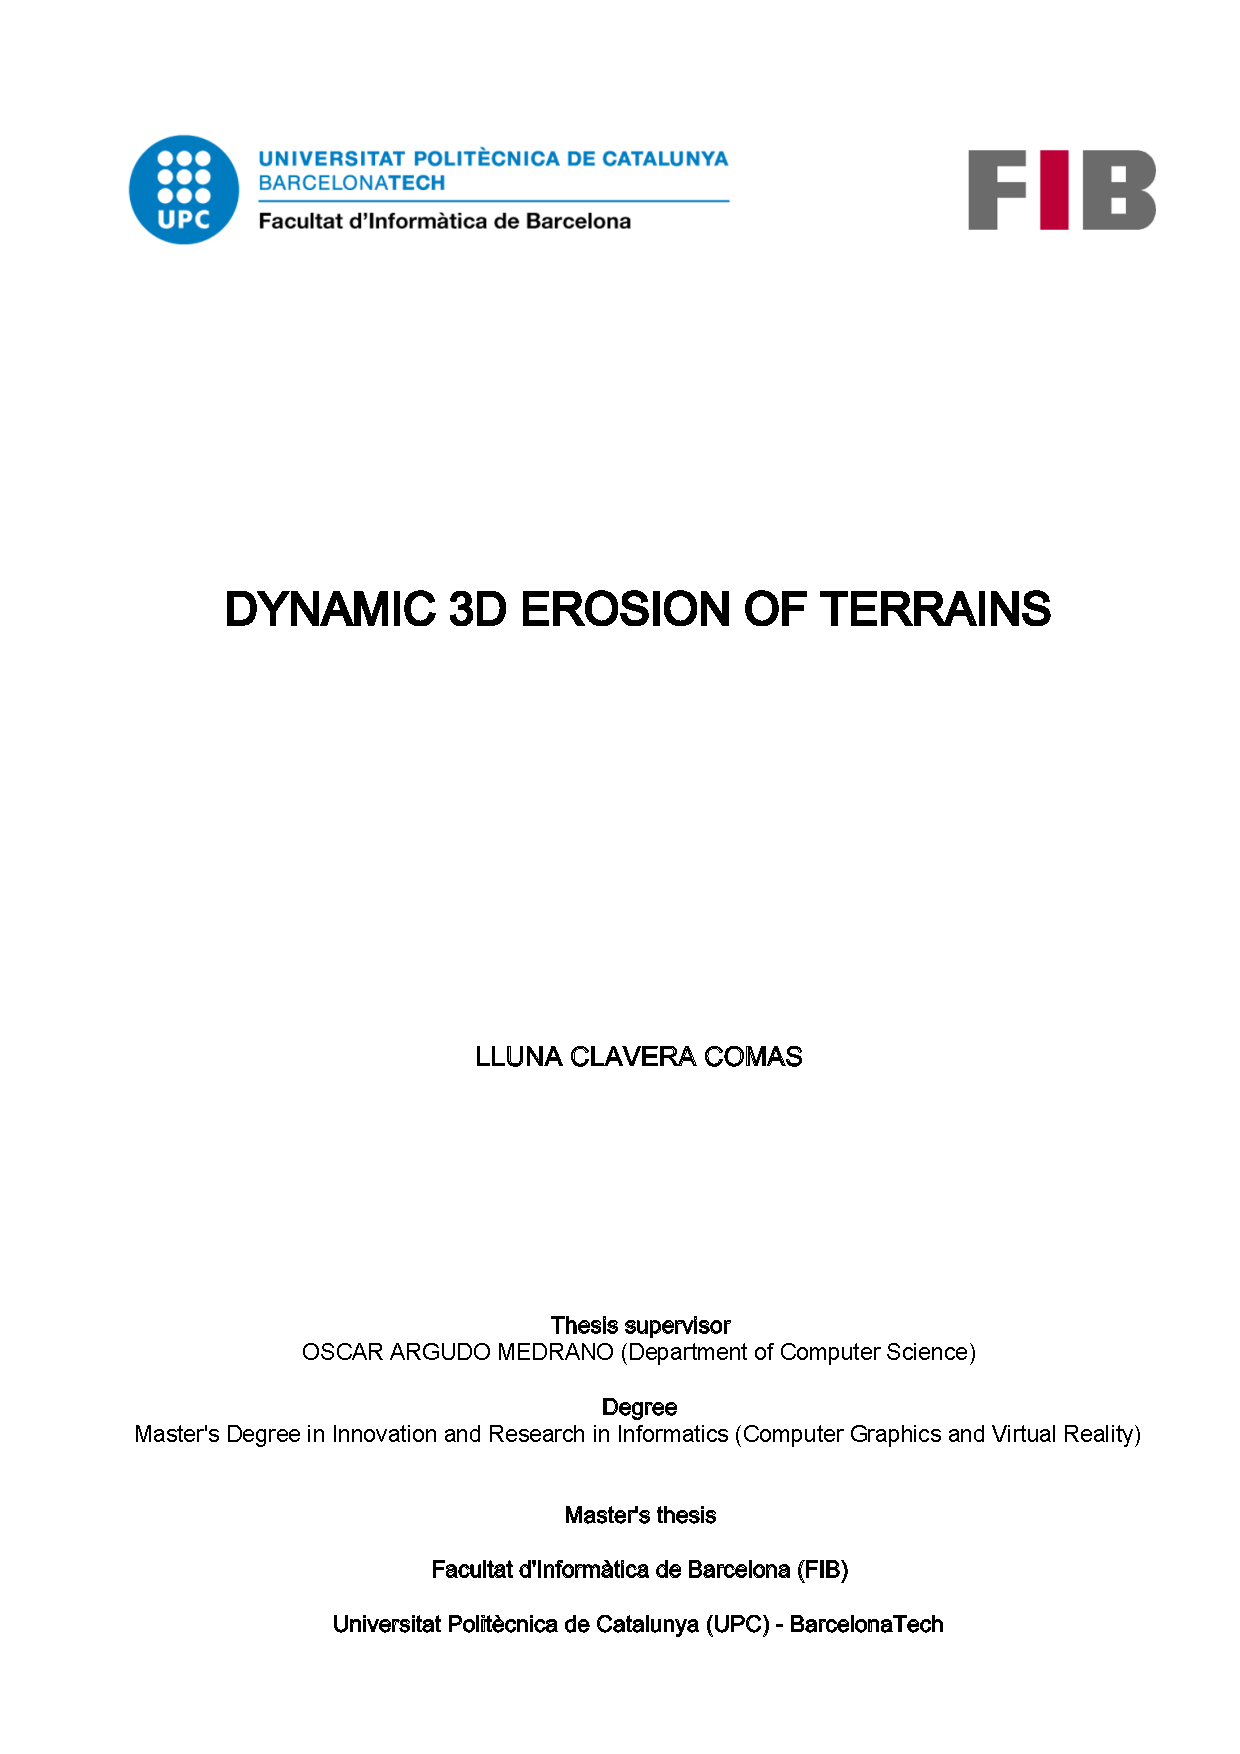
\includepdf[pages=-]{Title/portada.pdf}

\begin{abstract}
Erosion simulation is a core aspect of terrain synthesis, analysis and 
enhancement, as it allows us to recreate complex structures found 
in natural landscapes. The goal of this project is to improve previous erosion methods based 
on water infiltration to increase 
their quality and their realism. To achieve this, we propose a mechanical 
model to better simulate the state of a terrain and use it to improve 
the results of the erosion process. 

\vspace{10pt}

Additionally, we also propose an improvement on the generation of 
voronoi tessellations over Digital Elevation Models (DEMs), which is a core 
aspect of many erosion simulation algorithms.
\end{abstract}

   
   
\newpage
   
   
    
   % \renewcommand{\abstractname}{Acknowledgements}
   % \begin{abstract}
   
   % % First and foremost, I want to express my immense gratitude to Antoni Lozano for stepping up to be my supervisor and for coming up with the idea for this project. His $\Theta(2^n)$ wisdom has been really helpful in completing this bachelor's thesis. I also want to emphasize my deep appreciation for Antoni Lozano as both a person and a researcher.
   % % \\
   
   % % I also wish to extend my sincere appreciation to two individuals who have profoundly influenced my journey in the field of computer science: my dear friend, Víctor Franco, and my dedicated professor for PRO2, EDA, and Algorithmics, Conrado Martínez. Their mentorship and support have played a pivotal role during my Computer Science journey.
   % % \\
   
   % % And last but not least, big love to all the friends I've made during my time studying for this Computer Engineering degree.
   % \end{abstract}
   
   % \newpage
   %\renewcommand{\epigraphsize}{\small\itshape} % Adjust the font size and style of the quote
   %\renewcommand{\textflush}{flushright} % Align the quote text to the right
   %\renewcommand{\sourceflush}{flushright} % Align the quote source to the right
   %
   %\renewcommand{\epigraphrule}{1.1pt} % Remove the line between the quote and the author
   %
   %\epigraph{Hola Cuca}{DJ Diva}
   %
   %
   %
   %
   %\newpage
   %
   \setlength{\headheight}{45pt}
   
   \pagestyle{fancy}
   \fancyhf{}
   \rhead{\fontsize{9bp}{9bp}\selectfont{Dynamic 3D Erosion of Terrains}}
   \lhead{
\includegraphics[width=215px]{Title/logo-upc.png}}
   \rfoot{\thepage}
   \setstretch{1.25}
 % \newgeometry{
 % a4paper,
 % left=20mm,
 % top=30mm,
 % }


\tableofcontents
\listoffigures
\listoftables
\chapter{Introduction} \label{intro}

Virtual terrains appear in a wide variety of applications: from entertainment
to physical simulation or science visualization, a lot of virtual scenes 
are set on a digital landscape. Despite the ubiquity of virtual terrains 
on 3D scenes, the complex and fractal structure of natural landscapes still
brings multiple challenges for the field of synthetic terrain generation.

\vspace{10pt}

Most virtual terrains are represented using 2D heightfields which, despite 
being highly convenient when generating, storing and manipulating terrain
models, have a major drawback: heightfields can only represent 2.5D 
models. Because each point in a 2D plane has a set elevation and every 
point between the ground and the given elevation is considered as solid 
(and the terrain interior), we can not represent features like caves, 
arches or overhangs, where not all points between the ground and the 
maximum elevation are solid. Additionally, these representations of terrains 
also fail to reproduce complex geometry commonly found in rocky terrains, 
like sharp ridges, loose blocks or steep cliffs.

\vspace{10pt}

Many of these complex structures that can not be easily captured by 2D 
heightfields, arise from different types of weathering events, like percolation
and freeze-thaw cycles. To address this limitations on virtual terrain models,
our goal in this thesis is to study the mechanical weathering of rocky 
terrains to enhance models given from 2D heightfields and add the complex features 
that these fields fail to capture. 

\vspace{10pt}

Terrain enhancement through weathering simulation not only improves the 
realism and quality of the models, adding the aforementioned complex 
features, but it can also be applied dynamically to simulate the changes 
a terrain goes through over multiple years.

\vspace{10pt}

This project is built on a previous project on this same topic \cite{10.2312:ceig.20241139}. 
Using the same algorithm as a base, we worked on addressing some of its 
limitations and improving both its quality and efficiency.
\section{Contributions}

As we just mentioned, this project is heavily based on a previous one, and
our proposed algorithm is built on the method they proposed. Despite that, 
in this thesis we will provide 
multiple improvements to the base algorithm to address some of its limitations. 

\vspace{10pt}

The main point we wanted to address of the previous project was the lack of
a physically based approach to the algorithm, as the proposed algorithm
made a lot of simplifications and ignored multiple physical interactions 
which made the method less accurate and realistic. However, during this 
thesis we also found other areas that could be improved and expanded, 
which also took a significant ammount of effort to solve.

\vspace{10pt}

The limitations of the previous project and our improvements will be 
discussed at length during this thesis, but our main contributions can
be summarized in two large blocks: improvements to the decomposition of 
the terrain into cells and
improvements on the quality of the algorithm by including a mechanical 
model to the simulation.  

\section{Set-up and tools}

Another difference between the project we base this thesis on, albeit less
significant, resides in the tools used. In the project that presented the algorithm we 
are extending, a blender plugin was implemented to show the method, however, 
here we have implemented our erosion simulation algorithm using C++ and we showed the 
results in a QT application using OpenGL for rendering.

\vspace{10pt}

To make the application, we reused the code provided by an article on 
terrain descriptors \cite{Argudo2025descriptors}, as it already 
implemented many basic functionalities to work with virtual terrains. We
then modified and expanded the application implementing our algorithm for 
mechanical weathering as well as implementing other functionalities to aid in the 
visualization and debugging of our method. Some of the changes that we 
implemented modify the basic functionalities of the program, so 
our project should not be seen as an extension to said application.

\vspace{10pt}

Finally, we used the C++ library Voro++ \cite{osti_code-54674} to generate 
voronoi decompositions, a core aspect of our erosion algorithm.
\newpage
\chapter{Preliminaries}

To understand this project and our contributions to the field, we will 
first present some background information about the topic, so that the reader 
can better understand both the problem and our proposed solutions.

\section{Terrains and Landscapes}

T
\subsection{General weathering effects}

\subsection{Freeze-thaw cycle}

\section{Terrain Representation and Modeling}
Virtual terrains are a fundamental aspect of this thesis, so it is important 
to review current approaches to represent and work with these types of models.
A deep dive into the state-of-the-art on terrain generation can be found on 
\cite{galin2019review}, but we are going to present only the most relevant 
methods for our project, as a full review is out of the scope of this thesis.

\subsection{Terrain Representations} \label{TerrainRep}

When representing terrains and landscapes there are multiple data structures 
and representations we can use depending on the ammount of information that 
we need to store and the nature of the model.

\vspace{10pt}

The main model representation techniques can be divided in \textit{Elevation
Models}, maninly focused on representing the surface of the terrain, and 
\textit{Volumetric Models}, that aim to capture some interal properties of 
the terrain as well as more complex structures.

\subsubsection{Elevation Models}
Elevation models are the simplest ways of representing virtual terrains. 
They consist on assigning an height to every point on a 2D space. In a more 
formal way, a terrain is represented by a function $h: \mathbb{R}^2 
\rightarrow \mathbb{R}$ that is at least $C^0$. From an height function we 
can easily extract the slope at one point $s(x,y)$ by using the norm of 
the gradient:

$$s(x,y) = \left \lVert \nabla h(x,y) \right \rVert = \left \lVert(\frac{\partial h}{\partial x}, \frac{\partial h}{\partial y}) \right \rVert$$

And from the gradient (projected to $\mathbb{R}^3$) we can easily obtain 
the normal at one point $n(x,y)$:

$$n(x,y) = \frac{(-\frac{\partial h}{\partial x}, -\frac{\partial h}{\partial y}, 1)}
{\left \lVert (-\frac{\partial h}{\partial x}, -\frac{\partial h}{\partial y}, 1)\right \rVert }$$

With the height, normal and slope we have all that we need for a basic 
representation of a terrain. Of course, as we are using a bivariate function
to represent the terrain, we can only have one elevation for each point 
on the domain, and that makes features like caves or overhangs impossible 
to represent with this method.

\vspace{10pt}

Despite its limitations, elevation models are widely used for its simplicity
and memory efficiency as they can capture the general structure of a landscape,
given that complex features like overhangs often represent a small part of the 
overall terrain.

\vspace{10pt}

To expand on this topic, elevation models only require a bivariate function
to represent the whole terrain, which can capture the whole terrain in a 
really simple closed-form expression, providing infinite precission with 
an extremly small ammount of memory. However, constructing functions that
represent complex realistic terrains is highly challenging and, for that 
reason, elevation models commonly use \textit{discrete heightfields} 
(also called \textit{Digital Elevation Models} or DEM) to represent terrains.

\vspace{10pt}

Discrete Heightfields are a collection of altitudes in a 2D grid. In order 
to create a DEM, you have to divide the domain of the terrain (assuming a 
rectangular domain) into a grid of $n x m$ cells, then, you assign an altitude
to every cell of the grid. The grid will only contain concrete values for
a set of discrete values, but you can obtain a height for every point of 
the domain by interpolating multiple values of the heightfield. This method
limits the accuracy of the model (as we stop having infinite precission), 
but it has the advantadge of representing arbitrary terrains in a really
simple way.

\vspace{10pt}

Heightfields are an extremly common way to represent terrains, and they can
be easily stored in textures and monochromatic images (as figure 
\ref{fig:anetoImage} shows), sometimes making use of the texture 
interpolation capabilities on the GPU to accelerate computations on 
heightfields. Specifically, DEMs are used on \cite{Argudo2025descriptors}, 
a project focused on terrain analysis that provides multiple metrics for 
terrains and whose code has been1 reutilized in this project to implement 
and test our erosion algorithm.

\begin{figure}
    \centering

    \subfigure[Aneto heightfield]{\label{fig:anetoTex}
\includegraphics[width=0.28\linewidth]{Background/aneto.png}
    }
    \hspace{20pt}
    \subfigure[Aneto model on the app]{\label{fig:anetoApp}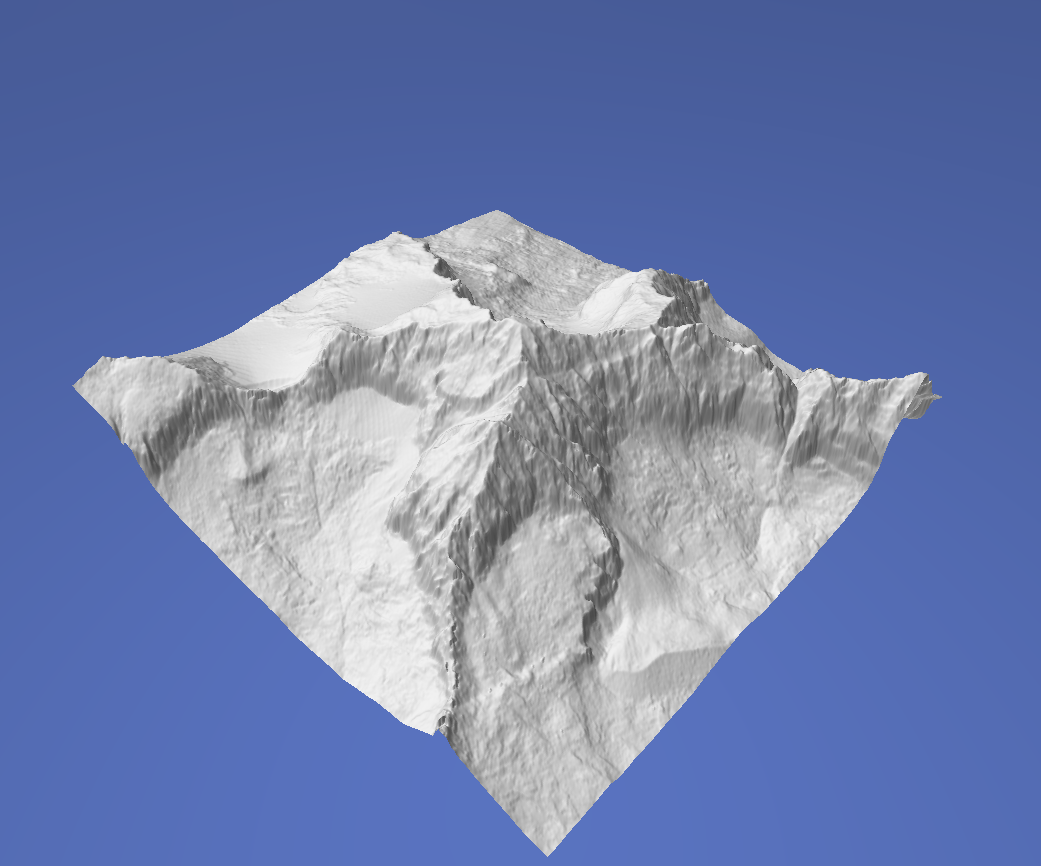
\includegraphics[width=0.335\linewidth]{Background/aneto-app.png}
        }
    
    \caption{Heightfield of the mountain Aneto as a monochromatic image and 
    the terrain produced by said heightfield on our application}
    \label{fig:anetoImage}
\end{figure}

To finalize the topic of elevation models, they have been extended to 
represent some internal structure of the model by employing a layered 
represesentation of the terrain. Layered representations are basically an 
ordered collection of height functions, each function representing a layer
of the model (which usually corresponds to a different material), resulting
in a stack of elevations for each grid cell. A representation of these 
types of layered heightfields can be seen on figure \ref{fig:layeredRep}

\begin{figure}
    \centering
    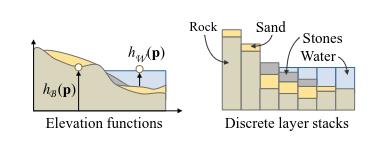
\includegraphics[scale=0.65]{Background/layeredRep.png}
    \caption{Illustration of stacked height functions,
    figure taken from \cite{galin2019review}}
    \label{fig:layeredRep}
\end{figure}

\vspace{10pt}

Layered representations have been used to simulate erosion (\cite{945341} 
and \cite{10.1145/3072959.3073667}) and, specially to simulate weathering 
events related to sediments as those types of rocks are naturally organized 
in layers. There are interesting works on this topics, but those will
be covered on chapter \ref{previousWork}

\subsubsection{Volumetric Models} 

As seen previously, layered representations are a way to represent 
different materials and properties of a terrains, but if we are really 
interested in encoding the internal structure of a landscape, we will 
have to use volumetric models. Volumetric models can be defined by a 
function $\mu: \mathbb{R}^3 \rightarrow \mathcal{M}$, where $\mathcal{M}$
denotes the set of materials used (air can count as a material). This 
function will be assigning every point of the 3D domain to a material, so
now complex structures like overhangs can be represented, as well as 
different internal compositions of the terrain.

\vspace{10pt}

Despite volumetric models being defined with a function, in practice we
will usually use a 3D grid with discrete samples and perform some
interpolation to obtain values outside the fixed grid points, similarlly
to what we did with DEMs. Each cell of the 3D grid is usually called a 
\textit{voxel} and the transformation of a model into a set of voxels a 
\textit{voxelization}. Voxelizations allow us to freely move and remove 
parts of the model, so they have potential to be used for algorithms that
change the structure of the landscape, like for erosion simulation, and 
they have been explored in the literature \cite{wingender2022simulation},
but they also have the huge drawback of being extremly expensive 
memory-wise. For that reason there has been a lot of work in the literature
making voxel representations more efficient (like adaptaive grids) or 
presenting novel ways to represent models encoding volumetric information.

\vspace{10pt}

For our purposes, we could have used a voxelization to implement our 
algorithm, but we decided that decomposing the terrain in voronoi cells 
would produce more natural results in a more efficient manner. The main 
concepts of the decomposition that we have chosen will be explained on 
section \ref{voronoiTheory}.

\subsection{Terrain Synthesis}

Terrain generation techniques can be divided in three main groups (although
it is common to employ methods from the three groups in the same project):

\begin{itemize}
    \item \textbf{Procedural Generation:} Procedural generation methods 
    artificially generate terrains from scratch by applying randomized 
    processes, like faulting or using noise. 
    \item \textbf{Example-based:} Example-based methods create virtual 
    terrains using scanned-data of real-world terrains.
    \item \textbf{Erosion Simulation:} Erosion simulations methods apply
    algorithms to simulate geomorphological processes when creating the 
    landscape.
\end{itemize}

Synthetic terrains usually can not represent all the complexity of a natural
landscape by procedural generation alone, and that is why erosion simiulations
are so important, not only in order to "predict" a future for the landscape 
but also to add realism on virtual terrains. Even example-based terrains
often fail to capture some aspects of the terrain they are trying to replicate, 
as scans have precission limitations (and the bigger the region you want 
to scan the more difficult it is to do it with accuracy), and erosion 
simulation can also intervene in those cases to add more complexity to 
the landscapes.

\section{Model Decompositions}
One of the core aspects of simluating erosion on 3D terrains is 
the model representation that we use. Any eroision simulation applied
on a 3D model will modfiy the model and its properties, so proper
data structures that allow for dynamic modifications of the model are 
key for these types of simulations. Additionally, applying erosion to an 
object also exposes the \textit{interior} of said object, so any model
representation that we use also has to encode some internal information of
the model, as internal points of a model might become part of the surface
at some point of the process.

\vspace{10pt}

In this section we are going to explain some of the decomopositons that 
can be applied to virtual terrains in order to convert the full model in 
a set of independent parts that can move freely to modify the overall 
landscape. We already mentioned voxalizations before 
(on section \ref{TerrainRep}), but due to voxelization limitations 
(mainly the memory cost), we explored more complex techniques to decompose
our models.

\subsection{Tetrahedralization}
As you might already know, every polygon can be divided into a set 
of trtiangles that exactly match the perimeter of the polygon. Triangulizations
can also be used to aproximate curved surfaces with arbitrary precission. 
In the case 3D polyhedra and volumes, tetrahedra are the equivalent of triangles,
we can aproximate any volume using terahedra, with more efficiency than 
with any other polyhedra (like cubes). 


\vspace{10pt}

We could use a tetrahedralization to decompose our terrain into tetrahedra and,
then apply our algorithm over those pieces, and we could even further divide 
the tetrahedra into more tetrahedra to adjust the granularity of the 
decomposition. The concept of tetrahedralization and tetrahedral meshas 
has been used to simulate erosion in the past \cite{turini2006simulating}, 
but we have chosen a differnt decomposition that has some advantadges over tetrahedralizations and produce more irregular 
shapes, which better represents the shapes we can observe in nature.

\begin{figure}
    \centering
    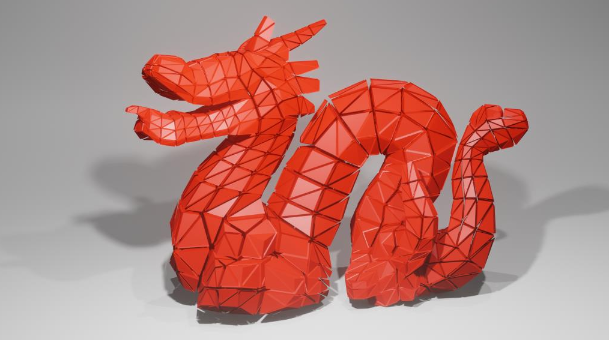
\includegraphics[scale=0.4]{Background/tetrahedralization.png}
    \caption{Example of a tetrahedalization, taken from \cite{Muller_2022}}
    \label{fig:tetrahedralization}
\end{figure}

\subsection{Voronoi Decomposition} \label{voronoiTheory}
Given a set of sample points, a voronoi decomposition is a partition of the space into 
multiple regions, where every region is defined by the set of all points 
that are closer to a given sample than any other sample. the boundary 
of every region (or cell), is given by the plane where every point of it
is at the same distance of two sample points.

\vspace{10pt}

In this thesis we decided to use voronoi cells for multiple reasons. First,
they can be generated with a lot of flexibility (just chose an arbitrary set 
of points) and we can adapt the decomposition depending on our needs. 
Additionally, the generated cells are not very regular, with varying 
sizes and shapes, which produces a more natural rocky appearance than
other more regular decompositions.

\begin{figure}
    \centering
    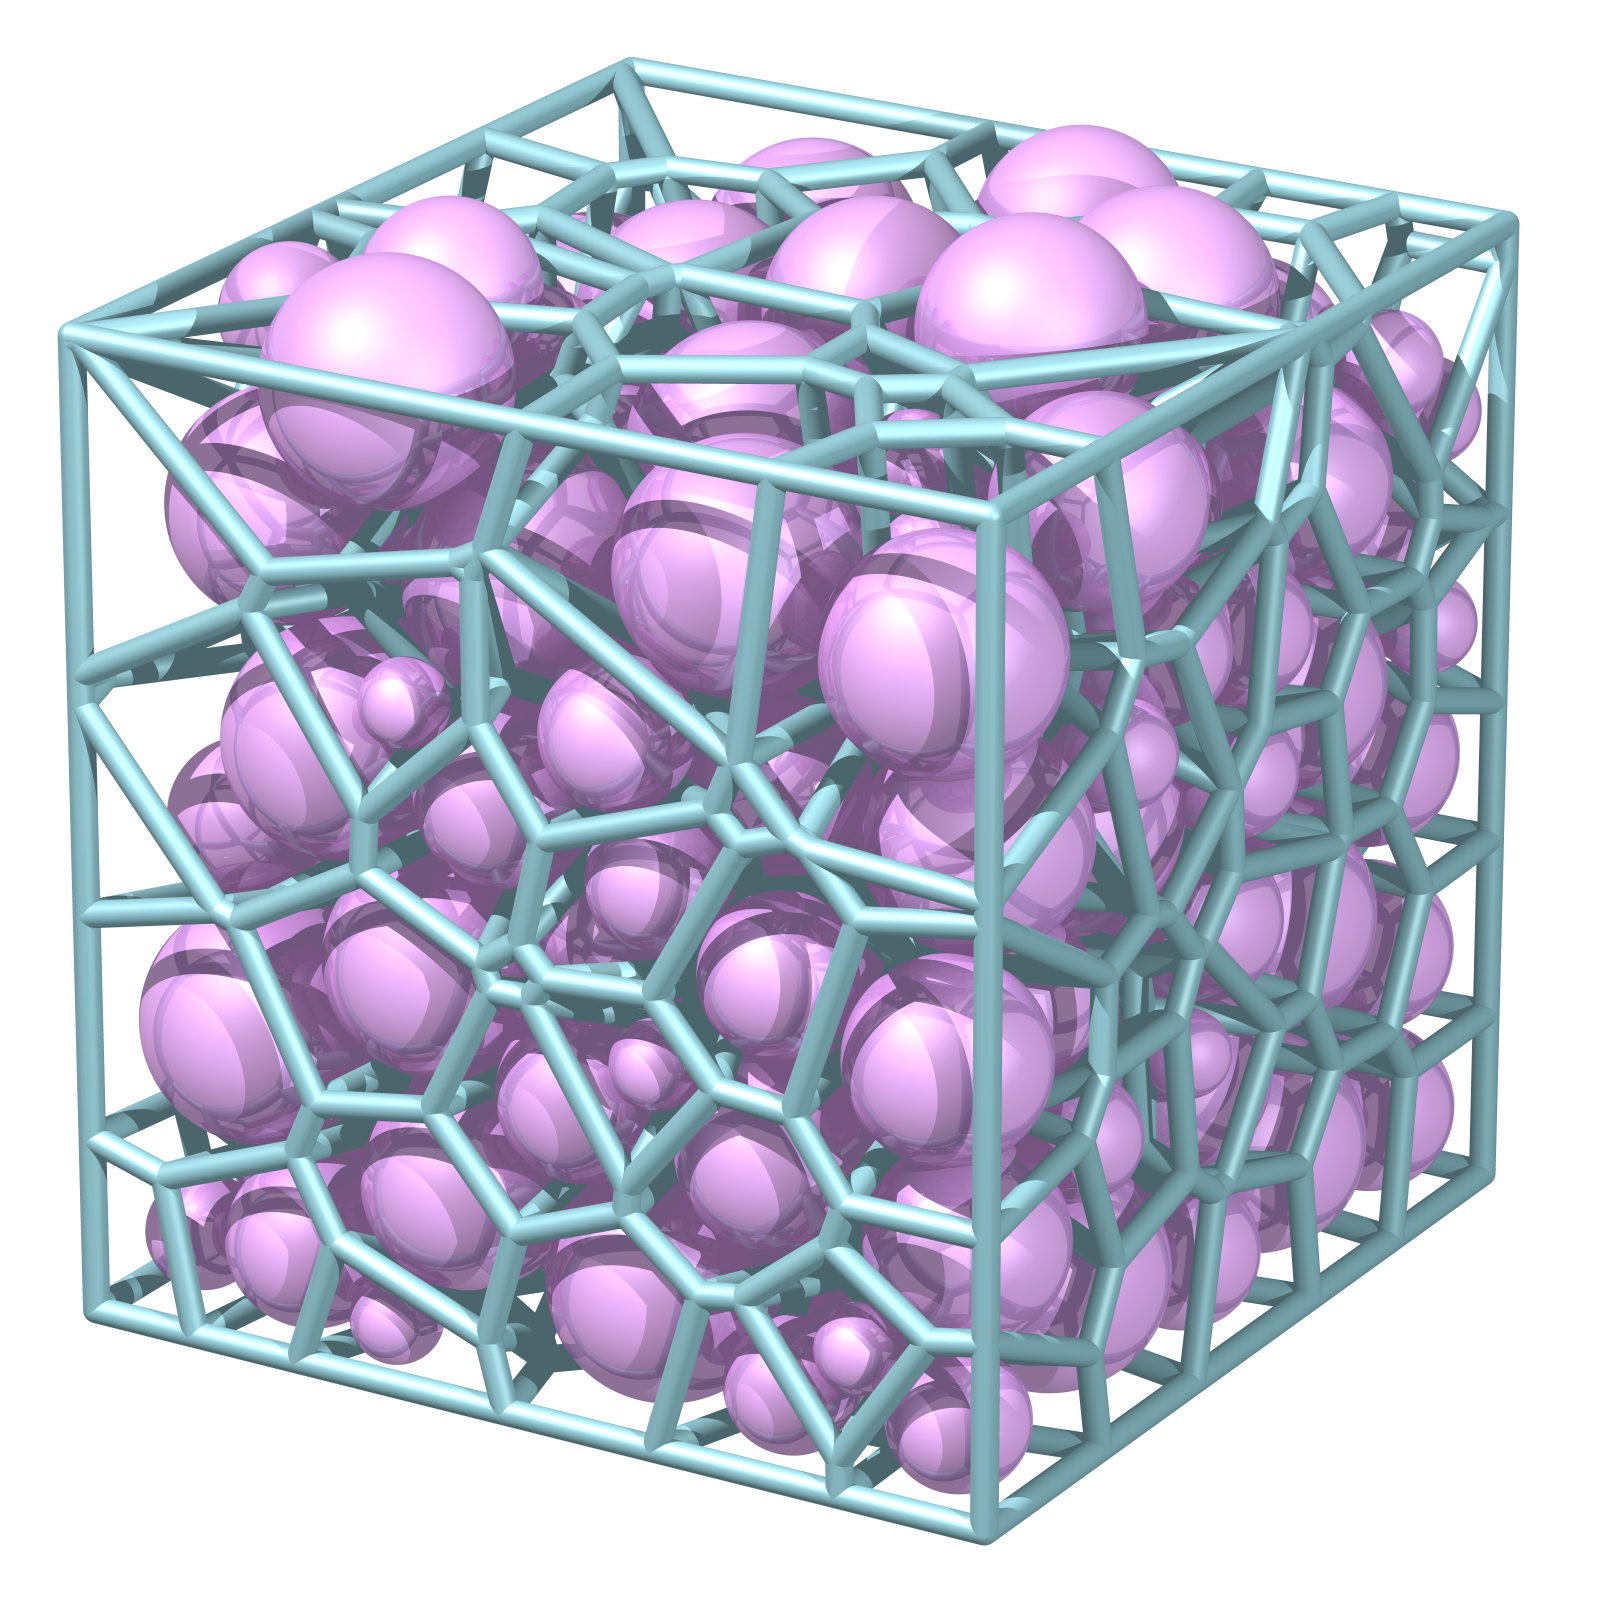
\includegraphics[scale=0.10]{Background/voronoiDecomp.png}
    \caption{Example of a voronoi decomposition of a cube, showing 
    the particles and faces of the decomposition. Figure taken 
    from the documentation of the C++ library Voro++ \cite{osti_code-54674}}
    \label{fig:voronoiDecomposition}
\end{figure}

\chapter{Previous Work} \label{previousWork}

There has been a multitude of proposed approaches to the problem of erosion 
simulation, each using different techniques and tackling different parts 
of the problem. To better understand our method and how it compares to 
previous solutions, we present a summary of the literature in the field, 
with their limitations and their differences with our approach. Additionally
we will also discuss the paper we are basing our algorithm on 
\cite{10.2312:ceig.20241139}, as our project can be seen as an extension to 
their work.

\section{Work in Applied sciences}
\subsubsection{Simulation of Crack propagation using eigenerosion}
\section{Work in Computer Graphics}
\subsection{Related Methods in Computer Graphics}

In this section we present work that is not focused on terrain erosion 
but it is still somewhat related to the topic.

\subsubsection{Spring-Mass Systems and Brittle Fracture}
Solid fracture is a fundamental aspect of simulating rock erosion, specially
when simulating the fractures caused by the infiltration of water and its 
freezing. To simulate breakage one common and simple approach is to use
spring-mass systems and remove overly extended springs. This approach was 
demonstrated years ago in \cite{10.1007/BF01900837} and \cite{10.1145/54852.378522}.

\vspace{10pt}

A more recent approach in this topic was presented in \cite{10.2312:sca.20141122},
where they explore the use of peridynamic systems for brittle fracture. 
Peridynamic systems are spring-mass systems with two particular properties:
they decouple stiffness from spring lenght and they also connect particles 
just by proximity instead of using 1-ring neighborhoods. An interesting 
part of the paper is that they have tried using Voronoi-Based Geometry 
to decompose the model and apply their spring-mass algorithm. In our case 
we also use voronoi-cells to generate our \textit{masses}, although the 
dynamics of the links and their fracture are different in our approach. 
Another approach that uses voronoi geometry for fracture can be found in 
\cite{10.1145/1242073.1242200}, although in this case they use voronoi polygons
over a surface instead of generating voronoi polyhedra in a volume.
\begin{figure}
    \centering
    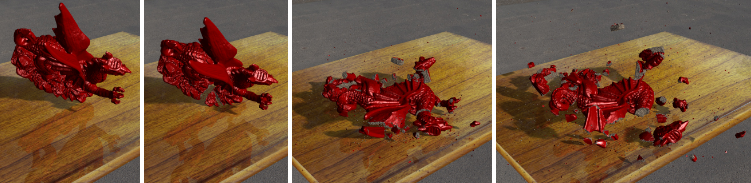
\includegraphics[scale=0.65]{Background/DragonBreak.png}
    \caption{A welsh dragon breaking. Taken from \cite{10.2312:sca.20141122}}
    \label{fig:dragonBreak}
\end{figure}
\subsubsection{Modeling Wood Decay}
Modeling realistic trees have some parallels to modeling terrains: The goal 
is to represent a complex natural object that is being constantly modified
through the interaction with its environment. Some work has been done \cite{10.1145/3641816}
\cite{10.1145/3721238.3730745} on simulating tree decay, which would be the equivalent of
simulating erosion on rocky terrains. 

\vspace{10pt}

On this specific topic, the recent work of \cite{YANG_SCHWARZ_2026} (which is yet
to be published on SIGGRAPH 2026) presents a really interesting method to 
simulate wood decay from fungal interaction. The method consists on 
dividing the tree model into \textit{segments} and then simulating a 
fungus infiltrating the host and generating fractures in the tree segments. 
A fungal infiltration also creates conditions facilitating further decay.
This is similar to the problem we are tackling: We divide a terrain into 
different components and then we simulate the water infiltrating the rock,
fracturing it and creating conditions where more water infiltration is 
favoured. The specific mechanics of rock fracture and wood decay are very 
different, so techniques for wood decay are not really applicable to our work, 
but the topic has interesting parallels.

\begin{figure}
    \centering
    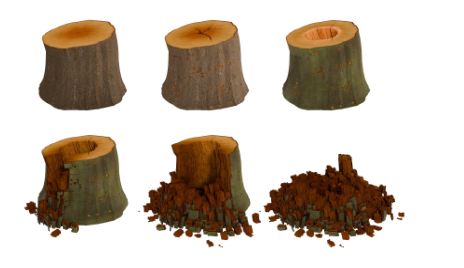
\includegraphics[scale=0.65]{Background/woodDecay.png}
    \caption{Example of wood dedcay of a cut tree trunk. Figure 
    taken from \cite{YANG_SCHWARZ_2026}}
    \label{fig:woodDecay}
\end{figure}
\subsection{Weathering in Computer Graphics}

Here we will show a summary of methods for erosion simulation in 
the literature.

\subsubsection{Physics-based Sandstone Simulator}

A recent approach to rock erosion was presented by \cite{10.1145/3731201}. The 
goal of the paper was to simulate sandstone dynamics with multiple effects like
wind and fluvial erosion. The presented method represents a sandstone structure 
using a set of particles and then they modify the model using the following 
equation for each particle:

$$\frac{\partial b}{\partial t} = -\varepsilon (\sigma_c) (\mathcal{W} + \mathcal{F})$$

Where $b$ represents the \textit{viability} which describes the 
expectancy that the rock has not been eroded, $\varepsilon$ represents 
the \textit{erodibility}, $\sigma_c$ is the Cauchy stress tensor, and 
$\mathcal{W} and \mathcal{F}$ represent the wind and fluvial local 
erosion effects. To compute that equation they divide te process into 
four parts: First they use the Material Point Method for stress computation 
and obtain $sigma_c$, then they compute the wind and fluvial erosion components, 
and finally they perform computations on deposition.

\vspace{10pt}

The problem solved by this simulator is similar to the one that we are 
tackling, but we are dealing with erosion by freezing and not with 
wind and fluvial erosion so our proposed solution will tackle other 
situations not covered by this method.


\begin{figure}
    \centering
    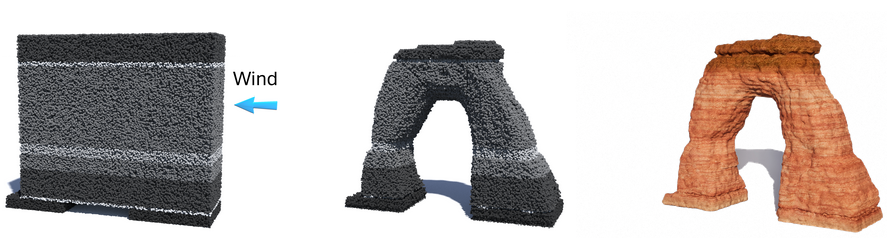
\includegraphics[scale=0.4]{Background/SandstoneArch.png}
    \caption{Arch produced by wind erosion. Figure taken from \cite{10.1145/3731201}}
    \label{fig:sandstoneArch}
\end{figure}


\subsubsection{Layered representations to simulate erosion}
In section \ref{TerrainRep} we briefly discussed layered heightfield 
represesentations andf how they can be used for erosion simulatio, 
specially to simulate sediments and their interactions. 
Using this strategy, the work of \cite{10.1145/3072959.3073667} presents an interesting approach, 
that specially focus in the interaction between vegetation and erosion and
their mutual interaction. In the paper, they divided the landscape in 
bedrock (unmoving), granular materials that may produce landslides and 
vegetation (dead and alive) and with that layered representation they could
run a simulation to modify those layers, representing the effect of 
erosion in the ecosystem, improving realism and showing the temporal 
evolution of a landscape. The layered representation they used can be 
appreciated on figure \ref{fig:layeredVeg}.

\vspace{10pt}

In our project we do not intend to deal with sediments and their interaction
with the environment, as the main erosion mechansim that we study is the 
one caused by water entering the pores of the rock and breaking them 
from inside, causing fractures and potentially separating chuncks of 
rocks from the main structure. Layered representations can represent
different features of the landscape with much more memory efficiency 
than other approaches and can also be used for erosion simulations, 
but they have limitations that make them not appropiate for certain 
types of erosion simulation, specially those that consider damage done 
on all the terrain and not just on the outer layers. 

\begin{figure}
    \centering
    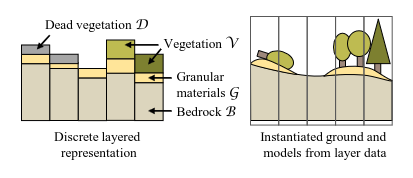
\includegraphics[scale=0.65]{Background/layeredVeg.png}
    \caption{Illustration of stacked height functions, used 
    to simulate interactions between vegetation and erosion. 
    figure taken from \cite{10.1145/3072959.3073667}}
    \label{fig:layeredVeg}
\end{figure}

\subsubsection{Machine Learning Approach}
In the field of terrain erosion there have also been approaches that use 
machine and deep learning to approximate the effect of erosion on a terrain 
and improve the realism of the landscape. In our work we do not use any of
these processes, so these methods are a little bit far of our proposed solution. 
Despite that, there are interesting solutions using this approach


\vspace{10pt}

In \cite{10.1145/3130800.3130804} they use a Conditional Generative Adversarial Network
trained on real-world terrain to add realistic detail to a rough sketch provided 
by the user, moreover, they also have a framework to simulate the evolution 
of the terrain through erosion (with another adversarial network); 
\cite{https://doi.org/10.1111/cgf.14992} presents an approach 
that procedually enhances terrains by adding erosion patterns using 
structured noise; and \cite{https://doi.org/10.1111/cgf.13345} uses Fully Convolutional Neural
Networks to upscale low-resolution terrains into plausible high-resolution 
ones.

\begin{figure}
    \centering
    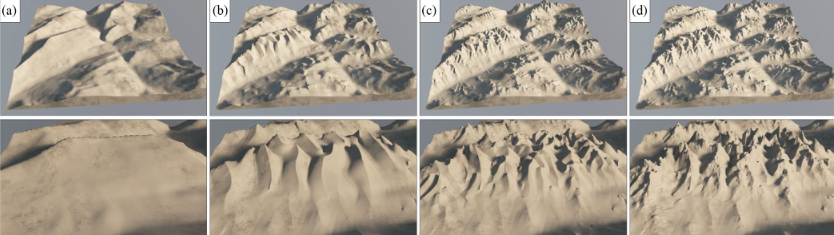
\includegraphics[scale=0.45]{Background/erosionDL.png}
    \caption{Example of terrain enhancenment through adding erosion patterns.
    Taken from \cite{https://doi.org/10.1111/cgf.14992}}
\end{figure}
\section{Base Simulator for this Project}

As mentioned on the introduction of this report (\ref{intro}), this thesis
is built upon the work of \cite{10.2312:ceig.20241139}, so we started from 
the algorithm they proposed and made some extensions and improvements. For 
this reason, in order to understand our projet we first have to understand
the method presented in the previous project.

\vspace{10pt}

In the paper, \cite{10.2312:ceig.20241139} present an approach to simulate
terrain erosion that can be divided into two main parts: first they divide 
the terrain into independent cells conected by \textit{links} between 
neighboring pieces, and, then, they apply an erosion algorithm to degrade 
the links and, eventually, remove the parts that have been disconnected 
from the terrain. Figure \ref{fig:waterInfiltration} shows the erosion 
simulation in action, with water infiltrating a terrain that has been 
decomposed into voronoi cells.

\vspace{10pt}

To perform the decomposition of the terrain into cells they sampled multiple
points of the model and then generated a voronoi tesellation. In our project
we still use the voronoi tesellation to generate the cell graph, but we 
modified the sampling to obtain better results. The original method used
boolean operations between the voronoi tesselation and the original model so
that the tesellation would fit the base terrain, but we tried to improve 
the decomposition so it could better fit the terrain without extra operations.


\vspace{10pt}

Regarding the algorithm that simulates water infiltration and link breakage, 
we implemented a mechanical model to represent link stress and modify 
those stress values once a link has been broken. This extension of the 
algorithm now modifies the state of the system after a fracture, instead 
of just modifying the state of one link, which can produce an effect called
crack propagation. The addition of this mechanical model makes the method 
more based in real natural processes and it improves its realism.

\vspace{10pt}

Additionally, we also experimented with multi-resolution decompositions in 
order to improve the efficiency of the simulation without compromising too
much on its quality. The algorithm can be applied in a less granular 
decomposition and then we can modify the more granular one according to the 
changes on the higher level.

\vspace{10pt}

Furthermore, this thesis also changes a lot the use tools and the testing 
framework. The original project implemented a blender plugin to demonstrate 
their solution, while we implemented the algorithm into a C++ OpenGL 
application.

\vspace{10pt}

Finally, even if the basic algortihm is taken from another project, we 
are going to explain in full detail all parts of the algorithm so that
the reader can understand our implementation just by reading this 
thesis. We are going to highlight our main contributions, but keep in 
mind some smaller details of the implementation may also be different 
to the original implementation (and we might not mention the change), 
as we took the main ideas of the method and implemented them in our own way.   
\begin{figure}
    \centering
    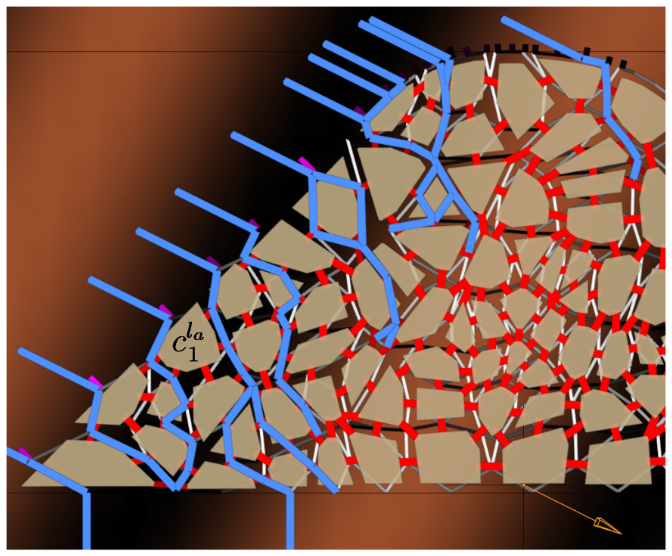
\includegraphics[scale=0.35]{Background/waterInfiltration.png}
    \caption{Example of water infiltrating a terrain divided into a set
    of voronoi cells connected by links. Taken from 
\cite{mateos_arlanzon_2023}}
    \label{fig:waterInfiltration}
\end{figure}



\newpage
\chapter{Model Decomposition}

In order to represent the internal structure of a model, we decomposed 
the base model into multiple cells covering the whole volume of the object.
A core part of this project has been focused on the model decomposition,
as well as on algorithms to produce and improve said decomposition. In this
section of the thesis we are going to take a deep dive into the basic method
taken from \cite{10.2312:ceig.20241139} and all the improvements we added.

\section{Base Method Overview}

As statet eariler, the main idea of the decomposition process is to divide
the original model into multiple shards that are connected with bonds (that 
we call links). In order to generate the fragments of the models, which 
will be called cells from now on, a voronoi tessellation is used, as they 
produce a more natural rocky appearance than other possible decompositions like 
voxelizations or tetrahedalizations. The process of generating is further 
divided in multiple steps: \textbf{Point Extraction}, \textbf{Voronoi Cells 
Generation} and \textbf{Links Generation}. Additionally we also experimented 
with multi-resolution decompositions, where one cell on the lower resolution 
contains multiple cells on the higher resolution level, this adds an additional
step that consists on creating the lower resolution levels from the higher one.


\vspace{10pt}

In the original project, they divided the decomposition process in different 
steps, as it can be seen on \ref{fig:Decomposition_diagram}, due to some changes
in the method we changed a the steps a little. Despite that, the main outline 
of the process is similar and our changes reside in the specific steps. 
 

\begin{figure}
    \centering
    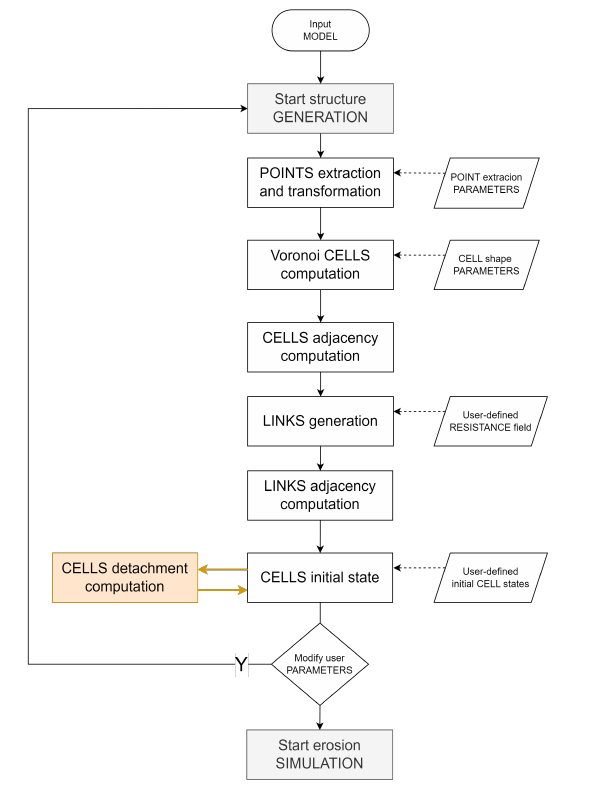
\includegraphics[scale=0.39]{Decomposition/BaseDecomposition.png}
    \caption{Diagram of the original method. Taken from \cite{mateos_arlanzon_2023}}
    \label{fig:Decomposition_diagram}
\end{figure}

\section{Point and Cell Generation}
Remember that voronoi tessellations are partitions of a model into 
different regions, where, given a set of centroids $C = \{c_1, c_2, \hdots , c_n\}$,
the set of regions $\mathbf{R} = \{R_1, R_2, \hdots, R_n\}$ is defined by: 
\begin{equation}
R_i = \{p \in \Omega | \forall c_j \in C, \; \;  d(p, c_i) \leq d(p, c_j)\}
\end{equation}
Where $\Omega \in \mathbb{R}^3$ is the domain of our model, $d$ represents 
the euclidean distance and $c_i$ is the centroid of region $i$.

\vspace{10pt}

This definition implies that the only thing we need in order to construct a 
voronoi tessellation is a set of centroids that will define our regions, then the 
regions will become our cells defined by the planes that form their boundaries. 
The number of centroids chosen and their positions heavily affect the result
of the tessellation, so the sampling method that we decide to implement will be 
highly relevant for the end result. In addition to the sampling, one more
thing that we will need to take into account is the fact that the regions
that lie on the boundary of the region will be technically unbounded and 
we will have to manually add walls to cut them so they do not leave the 
boundary of the original model.
 
\subsection{Cell Generation} \label{sec:cellGen}

The first step of the voronoi tessellation would be to sample the points 
that we will use as centroids of our cells. Despite that, we think it is 
better to first explain the process of constructing the cells from the 
points, as we took it into account when designing our sampling.

\vspace{10pt}

In order to construct the cells from the centroids we offload the computation
to the library Voro++ \cite{osti_code-54674}, which given a set of points 
and a boundary (with restrictions on the boundary that will be discussed 
in the future) gives us a set of polyhedra representing the different voronoi 
cells. Even if this part of the computation is offloaded to another library 
it is important to know about the process of construction of one voronoi cell.

\vspace{10pt}

Given a pair of centroids $c_i$ and $c_j$, the whole region is divided into 
two half-spaces: $H_{ij}$, where points are closer to $c_i$ than $c_j$; 
and $H_{ji}$, for points closer to $c_j$. More formally we can define $H_{ij}$
the following way: 

\begin{equation}
    H_{ij} = \{p \in \Omega | d(p,c_i) \leq d(p,c_j)\}
\end{equation}

Every point in $R_i$ is closer to $c_i$ than any other centroid $c_k$, so 
it follows that it also has to be in $H_{ik}$ for every $k \neq i$. Conversly,
if we have a point $p \in \Omega$ in $H_{ik}$ for every $k \neq i$, it follows that 
$p \in R_i$. This fact allows us to define the voronoi cell $R_i$ as the 
intersection of a set of hall-spaces:

\begin{equation}
    R_i = \bigcap_{j = 1}^n H_{ij}
\end{equation}

Each half-space is defined by the plane that is equidistant from both centroids,
so this converts the problem of creating a voronoi cell into computing the 
intersection of multiple planes. Keep in mind that $H_{ii}$ would define 
all the domain, since every point is at the same distance from $c_i$ and 
$c_i$, so it does not have any effect adding it to the intersection. A 
nice visual demonstration of the construction of a voronoi cell from 
the intersection of half-spaces is shown in figure \ref{fig:voronoiConstruction}

\begin{figure}
    \centering 
    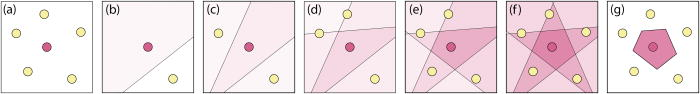
\includegraphics[scale=0.65]{Decomposition/voronoiConstruction.png}
    \caption{Process of construction of a voronoi cell from the intersection
    of half-spaces. figures (b) to (f) show the process of cutting the space 
    into multiple half-spaces, one half-space at a time. Figure taken from 
    \cite{10.1119/5.0087591}}
    \label{fig:voronoiConstruction}
\end{figure}

\vspace{10pt}

To end this section about constructing cells it is important to keep in 
mind that a pair of centroids define a plane where every point on the plane 
is equidistant from both centroids. Let us define this plane more formally, 
as we are going to use it later:

\begin{equation}
    P_{ij}  = P_{ji} = \{p \in \Omega | d(p,c_i) = d(p, c_j)\}
\end{equation}
\subsection{Point Sampling}
The first part of the method will be to sample multiple points inside 
the model to construct a voronoi decomposition. In this thesis, and 
unlike in the base method presented by \cite{mateos_arlanzon_2023}, we 
are using DEMs to represent and load our terrains, so we are going to make 
use of that. 

\vspace{10pt}

A heightfield $\mathcal{H}$ is basically a 2D grid were each
value $h_{ij}$ of the grid represents the height at one cell $(i,j)$ of the gird,
we can then use the points of the grid to obtain the elevation on a continuos domain 
using interpolation. Because we already have a defined grid, we can use 
it to implement our sampling. The main idea is to make use of the 2D grid 
and extend it to a 3D grid by setting a number of vertical samples (which 
will be a user-difine parameter) and then sample one point for each element 
of the grid, as long as the point lies inside the terrain (the 3D grid 
will represent the bounding box of the terrain, so not every voxel will be 
inside it). 

\vspace{10pt}

Now that we have a way to uniformly sample points inside the model, we can 
extend it and break the regularity a little bit by shifting each point by a 
certain quantity. Considering each point to initially be sampled at the 
center of its grid cell, we are going to shift each point by \textit{strictly}
less than half the cell size in a random direction, this way be will 
obtain a sampling in between complete random sampling (white noise) and 
a completly regular sampling, where we guarantee each point to not be to 
close or to far to another. Specifically, from each grid cell center $c_{ijk}$
we create our sample $c_{ijk}'$ using the following equation:

\begin{equation}
    c_{ijk}' = c_{ijk} + \begin{bmatrix} r_xs_x \\ r_ys_y \\ r_zs_z \end{bmatrix}
\end{equation}

Where $s_x$, $s_y$ and $s_z$ are the cell sizes on each direction (we can have 
rectangular cells) and $r_x$, $r_y$ and $r_z$ are three different scalars sampled 
uniformly at random such as $-\frac{1}{2} < -m \leq r_k \leq m < \frac{1}{2}$, where 
$m$ denotes the maximum ammount of shifting allowed and $k \in \{x,y,z\}$. If $m$ 
was $\frac{1}{2}$ then samples will be allowed to lie on the boundary of the 
grid cell, which could result in two samples being at the same place, that is 
why we set $m$ to be \textit{strictly} smaller than $\frac{1}{2}$. 

\vspace{10pt}

Moreover, we can bound the distance between two arbitrary points in terms 
of $m$ and the cell sizes $s_k$. Suppose $s_x$ is the smaller size, 
then the minimum posible distance between two samples $c_{i,j,k}$ 
and $c_{i + 1,j,k}'$ appears when $c_{i,j,k}' = (x + m s_x, y + \alpha s_y, z + \beta s_z)$ 
and $c_{i + 1,j,k}' = (x + s_x - m s_x, y + \alpha s_y, z + \beta s_z)$, so the distance 
is:

\begin{equation}
d(c_{ijk}', c_{i + 1,j,k}') = ||c_{i + 1,jk}' - c_{ijk}'|| = ||(s_x - 2ms_x, 0, 0)|| = s_x(1 - 2m)
\end{equation}
Following a similar logic, the maximum distance between $c_{i,j,k}'$  and its closest sample $c_{i + 1, j, k}'$,
will be when $c_{i,j,k}' = (x - m s_x, y - m s_y, z - m s_z)$ and $c_{i + 1,j,k}' = (x + s_x + m s_x, y + m s_y, z + m s_z)$ and the distance 
would be:

\begin{equation}
d(c_{ijk}', c_{i + 1,j,k}') = ||c_{i + 1,jk}' - c_{ijk}'|| = ||(s_x + 2ms_x, 2ms_y, 2ms_z)||
\end{equation}

But keep in mind that this maximum distance will only be reached when $i = 0$, as in any other case $c_{ijk}'$ would be closer to 
$c_{i - 1, j, k}'$ than $c_{i + 1, j,k}'$ (defining $c_{ijk}'$ and $c_{i + 1,j,k}$ as we did).
An analogous argument can be repeated with $s_y$ or $s_z$ as the smaller size.
\vspace{10pt}

To sum up, the method we have chosen to generate samples bounds the minum and 
maximum distances between a sample and its closest pair, so it combines some 
regularity that comes with using a grid with some randomness that breaks the 
monotony and creates more natural shapes.

INSERT A FIGURE WITH LONGEST AND SHORTEST DISTANCE CASES???
\subsection{Wall Construction}
The last consideration we have to make to create the voronoi cells is about 
what do we do with cells on the boundary of the terrain. The method 
proposed on \cite{mateos_arlanzon_2023} relied on boolean operations between 
the model and the set of voronoi cells to cut the boundary cells, but in this 
project we have tried multiple methods to appropiately create the boundary 
cells without relying on expensive boolean operations between models.

\subsubsection{Using Custom Wall Classes}
\subsubsection{Sampling out of Bounds}
\subsubsection{Using Additional Samples to Generate Cutting Planes}
As explained on section \ref{sec:cellGen}, every pair of samples define a 
plane $P_{ij}$ with all points that are equidistant from both samples. 
Additionally, we know that region $R_i$ will be cut by all planes $P_ij$ 
such as $i \neq j$, so we can use this concept in order to generate new 
cutting planes using more samples for the voronoi cell generation algorithm.

\vspace{10pt}

As we mentioned on the preliminaries \ref{TerrainRep}, we can sample 
normal vectors from DEMs, which means we can extract a plane from every
point of the terrain surface. 
\section{Link Generation}
\section{Multi-Resolution Extension}
\newpage
\chapter{Erosion}

\section{Initial Method}
\section{Multi-resolution}
\section{Physical Model}
\section{Extensions}



\newpage
\chapter{Implementation and Results} \label{sec:implementationResults}
All methods developed in this project have been implemented in a 
QT application that allows for testing and debuging the simulation. In 
this section, we are going to explain the structure of the application, 
describing which features are implemented, including the user tools used to control 
different parameters of the method. Additionally, we are going to 
show different results of our techniques, comparing  
different parameters and providing some benchmarks.

\vspace{10pt}

All code used for this project can be found on the 
\href{https://github.com/Lluna-CC/Modeling-Erosion}{GitHub page of the project} 
so everyone can check and test it. It is important to state that we reused the code from a previous 
project \cite{Argudo2025descriptors} (made by the tutor of this thesis). This 
previous project provides tools for terrain analysis and synthesis, so it 
has everything we need to load and work with terrains represented as 
DEMs. Many of the tools provided by the original code are irrelevant to our 
purposes, so we removed many functionalities; however, we left some tools 
for terrain analysis, as they still provide some utility for debugging. 


\vspace{10pt}

Finally, before starting this section, it is important to 
mention that all tests have been performed in a Linux system with the following specifications:

\begin{itemize}
    \item \textbf{Operating System:} Arch Linux x86\_64
    \item \textbf{Kernel Version:} 7.0.12
    \item \textbf{CPU:} Intel Core i7-12700K
    \item \textbf{GPU:} NVIDIA RTX 3070 Ti
    \item \textbf{Memory:} 32 GB
\end{itemize}


\section{Voronoi Decomposition}
Taking a terrain given by a DEM and converting it to a collection of voronoi
cells representing the same (or roughly the same) surface is one of the 
core aspects of this thesis. We have tested multiple methods and parameters 
to obtain the most quality possible with reasonable 
efficiency. In this section, we are going to describe the tools we provide 
the user with to experiment with the decomposition as well as an analysis 
and comparison of different methods and parameters tested. 
\subsection{User Interaction}

\subsubsection{Voronoi Generation Options}
First of all, the user has the option to load heightfields into the 
application using either ASCII files or pictures in PNG format. Additionally,
we have also provided some \textit{toy examples} that the user can 
load in order to test all algorithms and see extreme examples. The toy 
heightfields are designed so it is easy to see the process of both the 
decomposition and the erosion simulation, and therefore, they are also 
small. Most of the debugging process has been performed on these toy examples, 
and we left the real terrains for some final experimentation, as the final erosion 
algorithm can be quite heavy on more detailed terrains.


\vspace{10pt}

Once a heightfield is loaded into the application, the user has multiple 
options to modifiy the resulting decomposition. First, the most
direct way to control the results of the decomposition is the 
\textit{Voronoi Options} section (found in the voronoi window on the 
part of the UI at the right side of the application), as seen in figure 
\ref{fig:voronoiOptions}. This section 
has a button to compute the decomposition and also has the option 
to modify multiple parameters of the process. First, the lower resolution 
level is always automatically computed using the \textit{furthest points sampling}
described in \ref{sec:multiResolution}, and the number of points in the 
lower resolution layer is the total number of points divided by the 
\textit{Multi-Resolution factor} in the voronoi options. 

\begin{figure}
    \centering

    \subfigure[Voronoi options section]{\label{fig:voronoiOptions}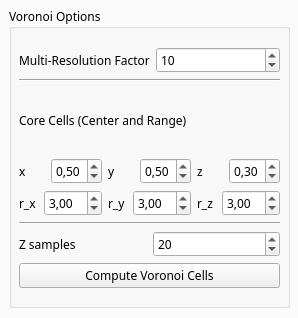
\includegraphics[width=0.28\linewidth]{Results/VoronoiOptions.png}
    }
    \hspace{20pt}
    \subfigure[Terrain dimensions section]{\label{fig:heightfieldDimensions}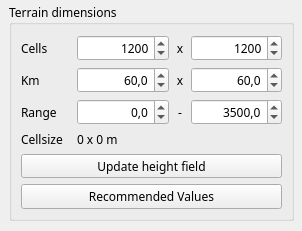
\includegraphics[width=0.35\linewidth]{Results/heightFieldSizes.png}
        }
    
    \caption{Voronoi options and Terrain dimensions windows of our applicaiton.
    Both windows can control the results of the decomposition}
    \label{fig:voronoiOptionsGeneral}
\end{figure}

\vspace{10pt}

Second, the user can also determine the generation of core cells (that will not be eroded
during the erosion algorithm). A rectangular block of core cells is 
always generated at a set position with a fixed size both specified by the user. The three parameters $(x,y,z)$ are numbers in 
the range $[0,1]$ and define the \textit{center} of the core cell block. The parameters 
are normalized using the bounding box of the terrain, so $(0.5, 0.5, 0.5)$ 
represents the center of the box. Next, $(r_x, r_y, r_z)$ define 
the \textit{range} of the core cell block. In order to normalize those 
values, they measure the range in \textit{cell sizes}; that is, $r_x = 2$
represents a value of 2 times the size of a grid cell in the x dimension.
When performing operations with the bounding box of the terrain, keep 
in mind that the bounding box of the decomposition extends a little 
bit beyond the highest peak in the $z$ direction so that we can take samples 
outside of the terrain.

\begin{figure}
    \centering

    \subfigure[Core cells when using center $(0.2,0.2,0.1)$ and 
    range $(1,1,1)$]{\label{fig:coreCells02_02_01_1}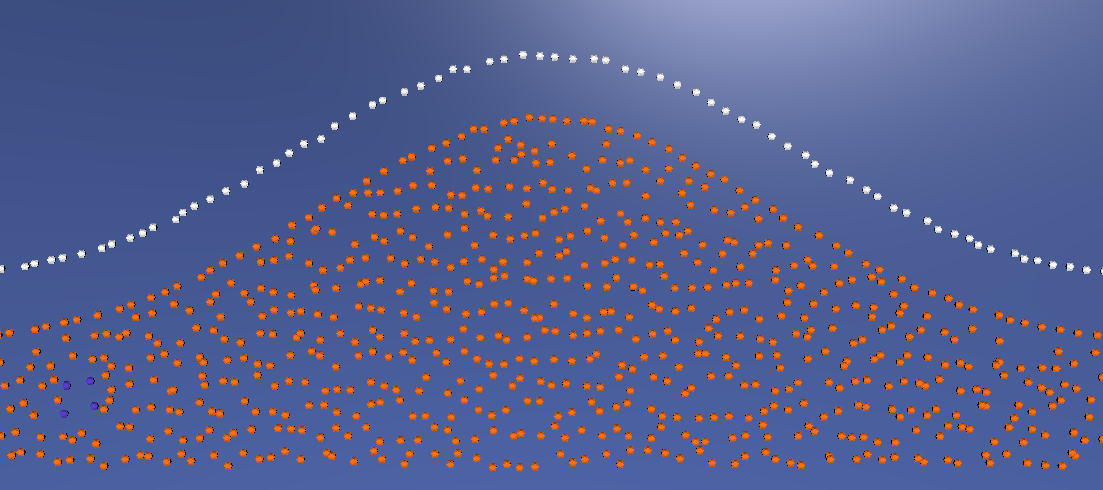
\includegraphics[width=0.45\linewidth]{Results/coreCells_02_02_01_1.png}
    }
    \hspace{20pt}    
    \subfigure[Core cells when using center $(0.8,0.8,0.1)$ and 
    range $(3,3,3)$]{\label{fig:coreCells08_08_08_3}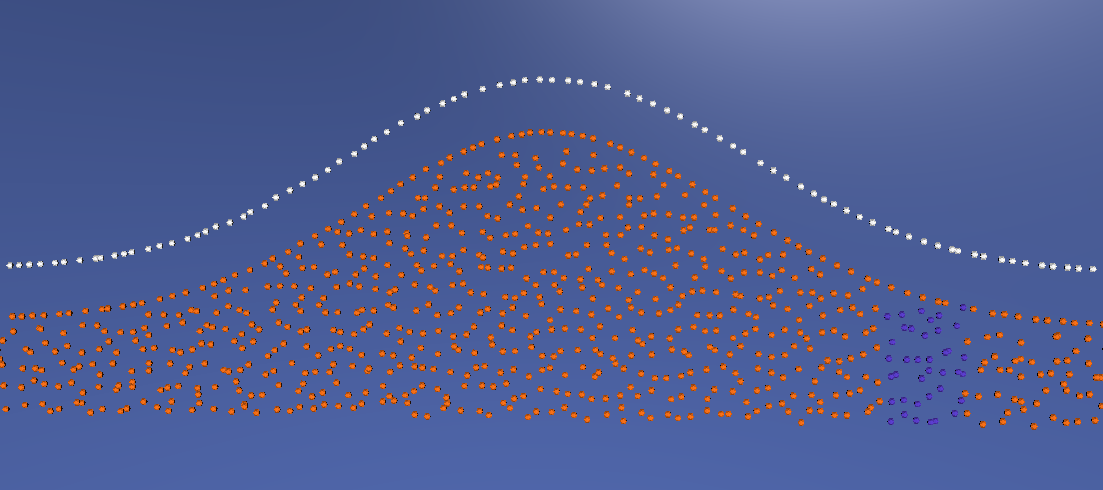
\includegraphics[width=0.45\linewidth]{Results/coreCells_08_08_01_3_2_3.png}}
    
    \caption{Results of modifying the parameters controlling the core 
    cell generation. Particles in purple represent core cells. Figure 
    taken using the \textit{Gaussian Bump} toy heightfield}
    \label{fig:voronoiCoreCells}
\end{figure}

\vspace{10pt}

Finally, the user has two options to modify the number of samples of the 
decomposition. The \textit{Terrain Dimensions} section 
on the left side of the UI (figure \ref{fig:heightfieldDimensions}) 
allows the user to modify the size of the heightfield. Because 
we are taking multiple samples for each cell of the heightfield, modifying 
the terrain dimensions will also modify the number of samples taken. 
Additionally, in the \textit{Voronoi Options} section, we can 
modify the \textit{zSamples} value, which will modify the number 
of vertical blocks of the 3D grid we construct to sample points.
As a final note, there is a button in the \textit{Terrain Dimensions} 
section called \textit{Recommended Values} that, for bigger terrains, 
will cap the dimensions (maintaining aspect ration) so they are feasible 
to compute. 

\begin{figure}
    \centering

    \subfigure[Salenques mountain sampled using a 256x184 grid (with 20 vertical samples)]{\label{fig:salenques256x184}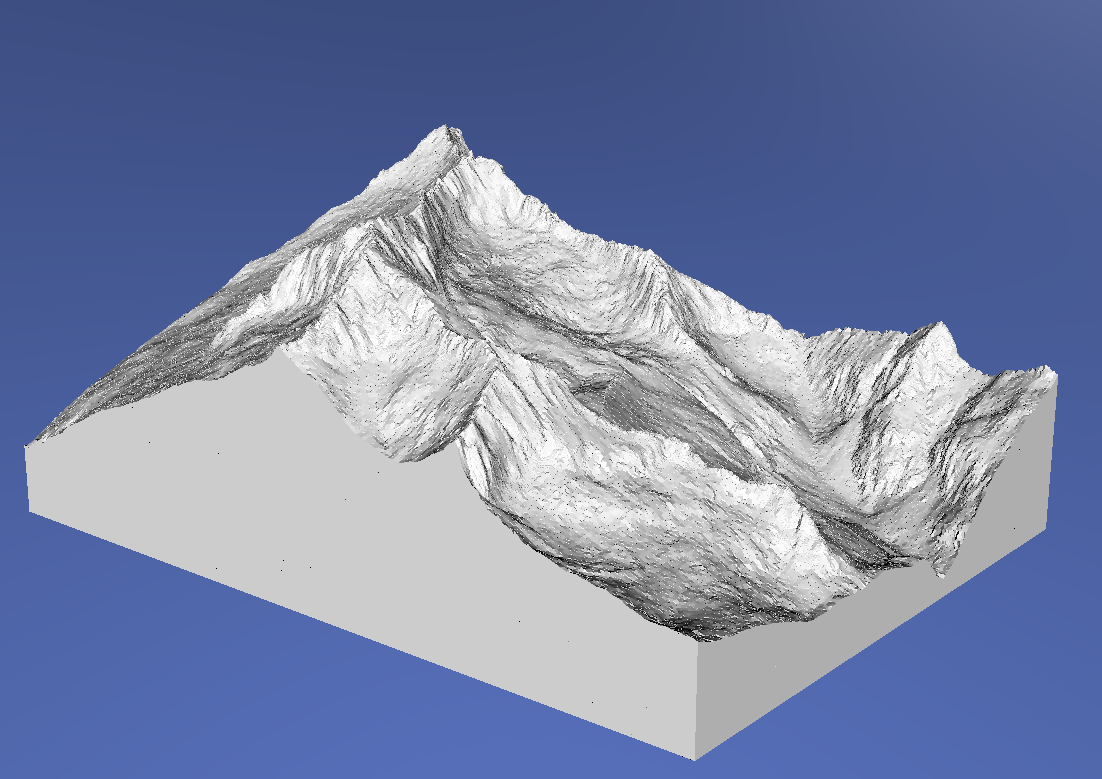
\includegraphics[width=0.4\linewidth]{Results/salenques256x184.png}
    }
    \hspace{20pt}    
    \subfigure[Salenques mountain sampled using a 64x46 grid (with 20 vertical samples)]{\label{fig:salenques64x46}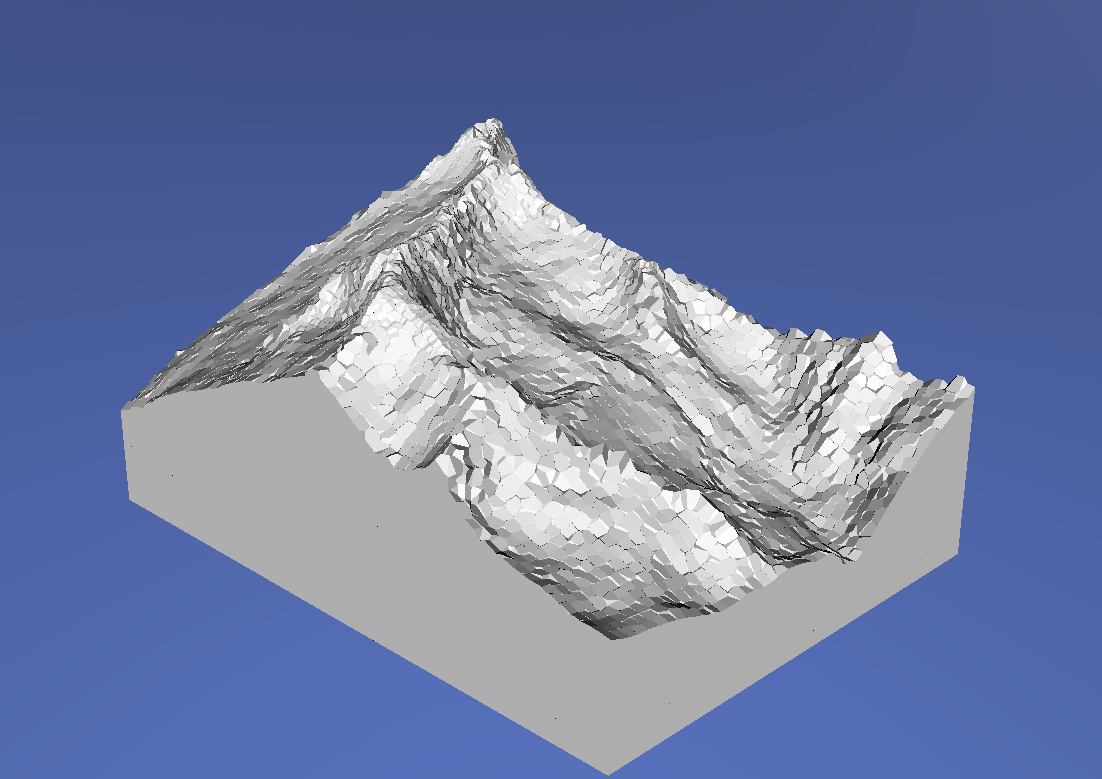
\includegraphics[width=0.4\linewidth]{Results/salenques64x46.png}}
    
    \caption{Results of modifying the heightfield dimensions on the terrain 
    Salenques}
    \label{fig:salenquesDimensionChange}
\end{figure}

\subsubsection{Visualization Options}

\begin{figure}
    \centering
    
    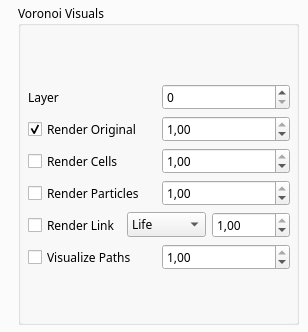
\includegraphics[scale=0.5]{Results/VoronoiVisuals.png}
    \caption{Voronoi Visuals section of the UI options}
    \label{fig:vorovisuals}
\end{figure}

In addition to the decomposition options, we also provided some options  
to visualize the results of said decomposition. Just above the 
\textit{Voronoi Options} section, there is a \textit{Voronoi Visuals} 
section (figure \ref{fig:vorovisuals}). Using these options we can 
visualize the original surface of the terrain, the decomposed terrain
made of cells, a visualization of the particles used to make the voronoi cells,
a visualization of the connections between cells (and their state, which 
will be useful when debugging the erosion simulation part), and a visualization 
of most recently generated water paths (also useful for the erosion 
part). The user can select multiple options to view multiple representations
simultaniously (like visualizing the original surface along other things, 
as seen in figure \ref{fig:particlesVsLinks}), and there is a variable 
next to each render option to modfiy the opacity of each of them. 

\begin{figure}
    \centering

    \subfigure[Example of the particle rendering mode]{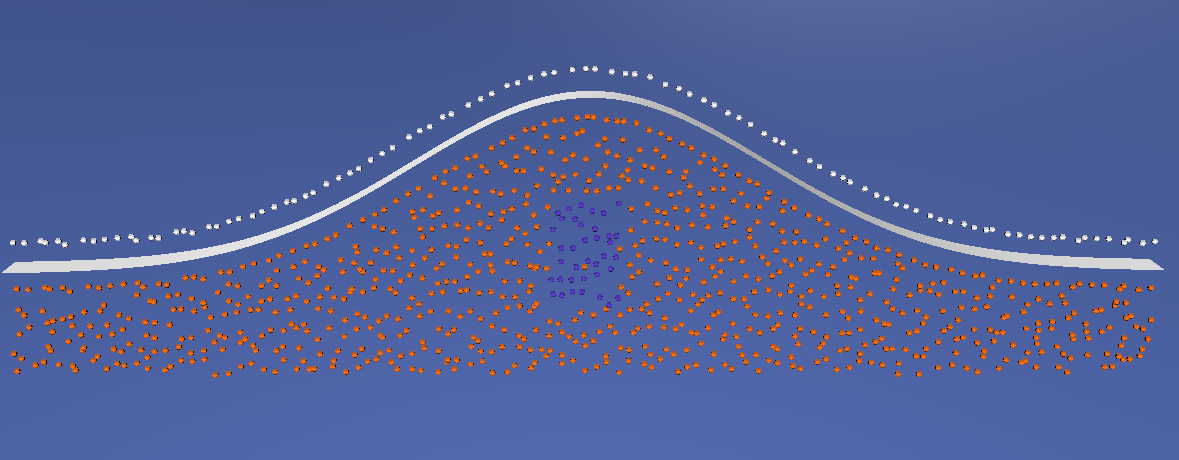
\includegraphics[width=0.35\linewidth]{Results/gaussianParticles.png}
    }
    \hspace{20pt}    
    \subfigure[Example of link rendering]{\label{fig:linksViz}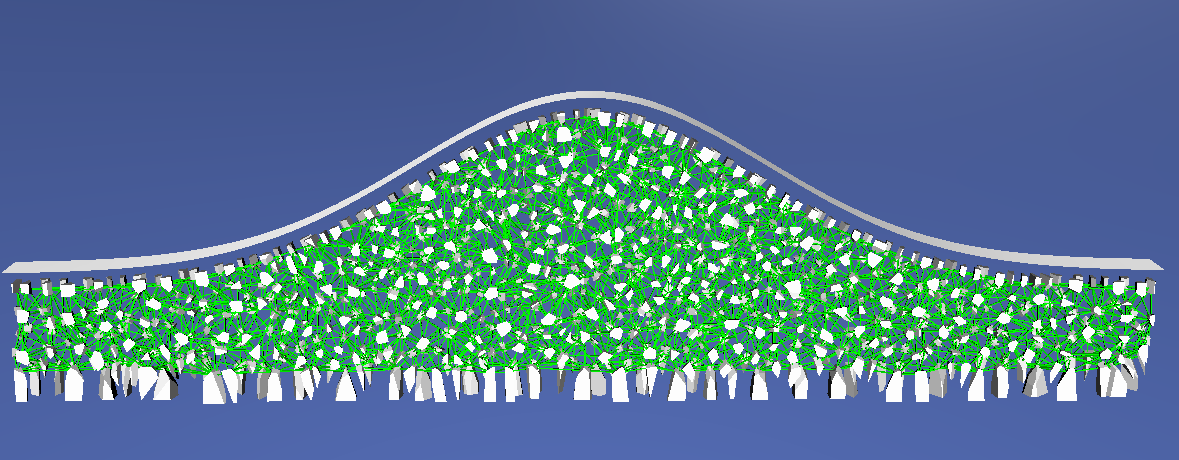
\includegraphics[width=0.35\linewidth]{Results/gaussianLinks.png}}
    
    \caption{Examples of diverse rendering options of our application. }
    \label{fig:particlesVsLinks}
\end{figure}


\subsection{Decomposition and Sampling Size Analysis}
In order to analyze our decomposition method, we performed multiple 
experiments varying the sampling size and the sampling method 
used to create the decomposition. By doing these tests, our 
intention was to better understand the relationship between 
the computational cost and the quality of the results, as well 
as to tune the parameters to obtain a good balance 
between cost and quality.

\vspace{10pt}

\subsubsection{Heightfield Dimensions Experiment}
Our first experiment tested the relationship between the heightfield 
dimensions (the base 2D grid) and the final results, both in terms of 
computation time and visual appearance. For this experiment we disabled
the cell subdivision protocol for high-rugosity cells, as changing 
the terrain dimensions might also have an effect on the rugosity, and 
we wanted to guarantee that the only changes to the model were the heightfield
dimensions. We also only used the terrain \textit{Punta Alta}, to avoid 
encountering differences between terrains.

\vspace{10pt}

We tried multiple sizes, and the results of the minimum, maximum and median 
tested dimensions can be appreciated in figure \ref{fig:2DdimensionResults}.
The terrain sampled using a 50x50 is really different from the other two, 
but the 200x200 does not have that much difference with the highest 
resolution tested, so it provides a good trade-off between efficiency and 
quality. 

\begin{figure}
    \centering

    \subfigure[Punta alta using a 50x50 grid]{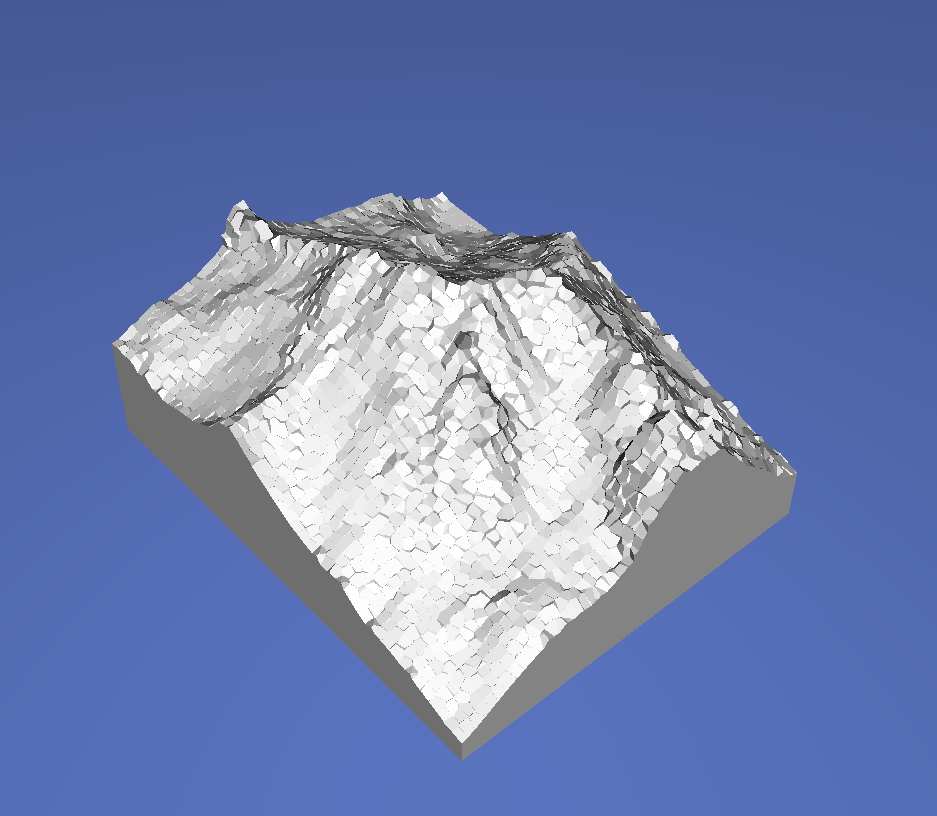
\includegraphics[width=0.3\linewidth]{Results/timeResults2D/puntaAlta50x50.png}
    }
    \hspace{10pt}    
    \subfigure[Punta alta using a 200x200 grid]{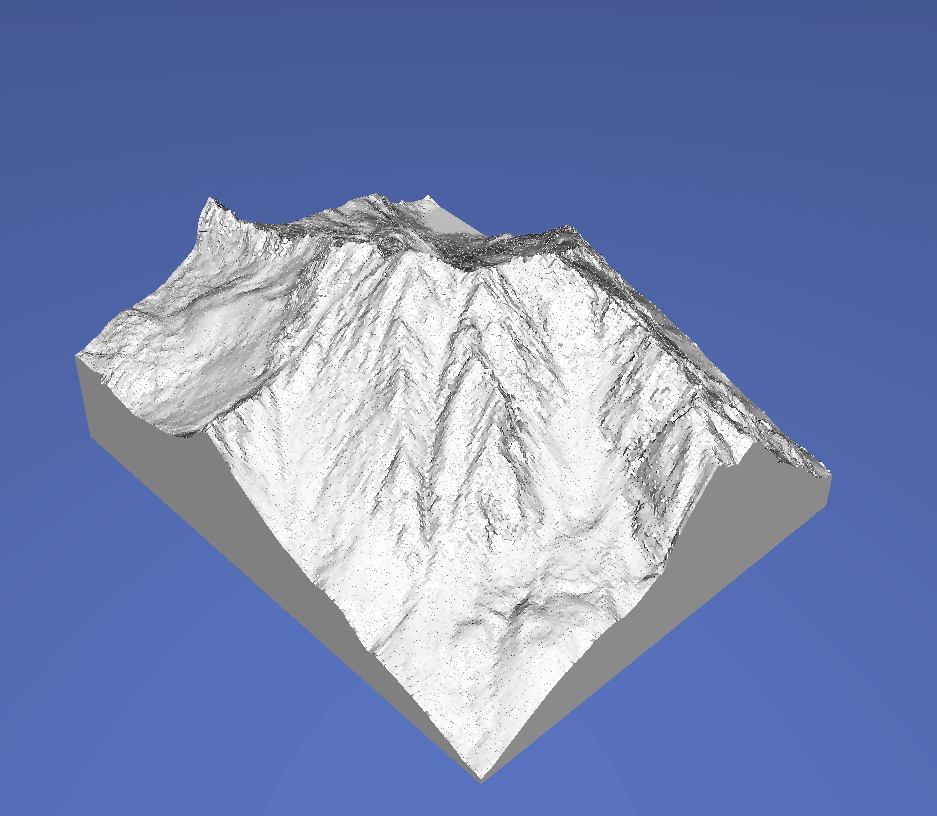
\includegraphics[width=0.3\linewidth]{Results/timeResults2D/puntaAlta200x200.png}}
    \hspace{10pt}
    \subfigure[Punta alta using a 350x350 grid]{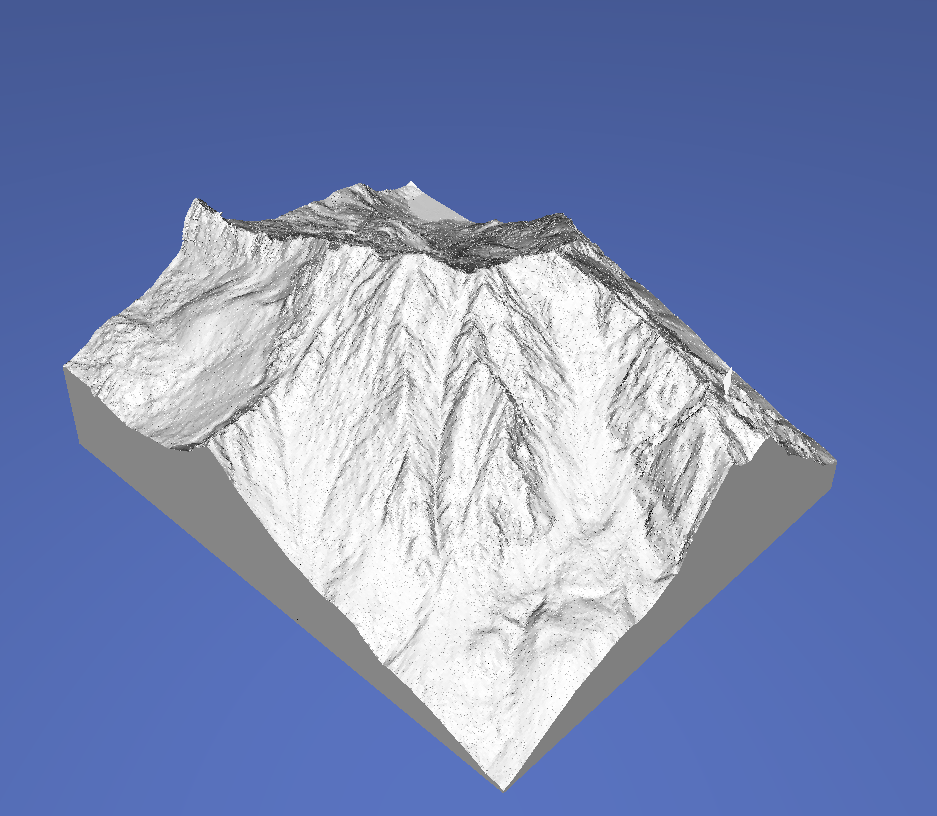
\includegraphics[width=0.3\linewidth]{Results/timeResults2D/puntaAlta350x350.png}}

    \caption{Results of modifying the heightfield dimensions in the terrain 
    Punta Alta}
    \label{fig:2DdimensionResults}
\end{figure}

\vspace{10pt}

Regarding the computational cost, if we consider a square heightfield NxN,
the number of particles generated is, of course, $O(N^2)$; however, the 
computation time is not as easy to determine. In the worst-case scenario,
computing a voronoi cell requires intersecting one plane for every other 
particle, so the computational cost would be $O(N^3)$. In practice, the library
voro++ \cite{osti_code-54674} implements this very efficiently, so this 
high theoretical cost might not appear in practice. In our empirical test, 
we found that the number of particles increased quadratically with 
the dimension $N$, but we also found that the time spent per particle 
also increased when increasing dimensions, so we can conclude that the 
relationship between number of particles and time is not fully linear.
These results can be seen in figure \ref{fig:2DtimeResults}. As a final note,
keep in mind that some aspects of the sampling depend on the terrain; as we 
avoid sampling outside the terrain, the number of samples in the z 
direction changes depending on the coordinates $(x,y)$, and the number 
of particles is not just $kN^2$ with $k$ representing the number of 
samples in the z direction.

\begin{figure}
    \centering

    \subfigure[Number of Dimensions vs Number of Particles]{
\includegraphics[width=0.35\linewidth]{Results/timeResults2D/dimensionParticles.png}
    }
    \hspace{20pt}    
    \subfigure[Number of Dimensions vs Time spent per Particle]{
\includegraphics[width=0.35\linewidth]{Results/timeResults2D/timePerParticle.png}}
    
    \caption{Results of modifying the heightfield dimensions in the terrain 
    Punta Alta on computation time}
    \label{fig:2DtimeResults}
\end{figure}

\subsubsection{Changing the Samples in the z-direction}

So far, we have only changed the dimensions of the heightfield, which is a 
2D grid. However, we sample points on a 3D grid, defined by the 
heightfield dimensions and the variable \textit{zSamples}. We also
experimented with this variable, and the results have been a 
bit surprising. The main factor of the visual quality of 
the decomposition is the accuracy at the surface, as anything below 
that cannot be seen until we perform erosion, which implies that 
increasing the number of samples in the z direction would be 
initially unappreciable (as seen in figure \ref{fig:zSamples10v99}). 
 

\begin{figure}
    \centering

    \subfigure[Results using $zSamples = 10$]{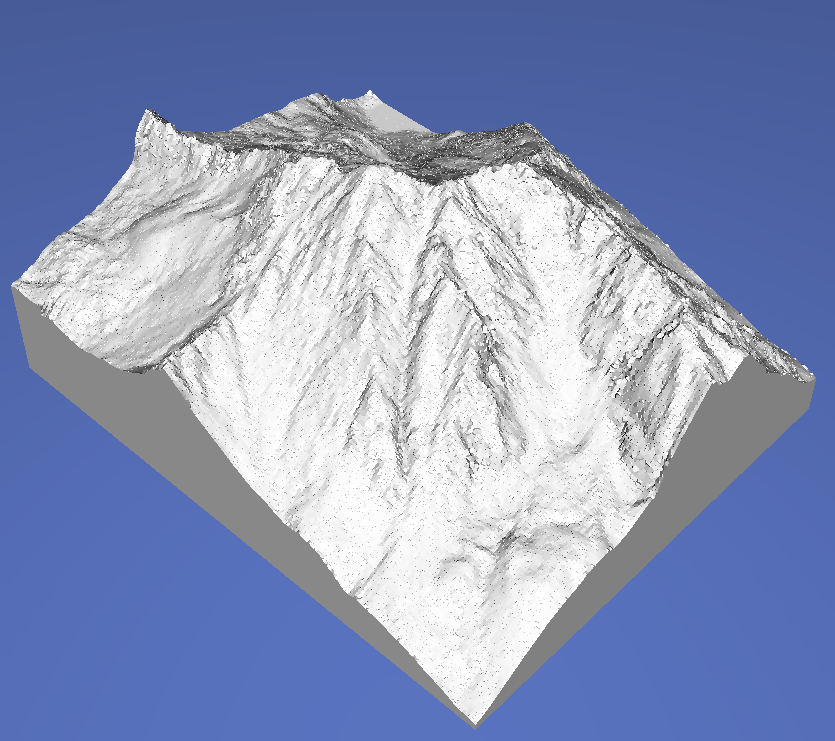
\includegraphics[width=0.3\linewidth]{Results/timeResultsZ/z10.png}
    }
    \hspace{20pt}    
    \subfigure[Results using $zSamples = 99$]{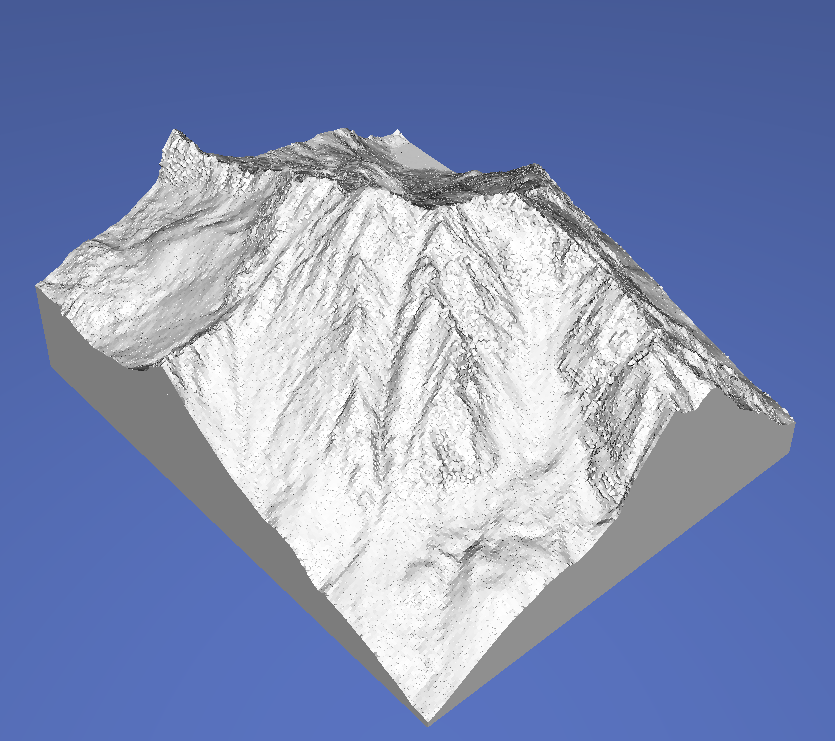
\includegraphics[width=0.3\linewidth]{Results/timeResultsZ/z99.png}}
    
    \caption{Results of modifying the variable $zSamples$ on the terrain 
    Punta Alta}
    \label{fig:zSamples10v99}
\end{figure}

\vspace{10pt}

The negligible effect on visual results was expected, but the unexpected 
part comes from the time spent to perform the decomposition. From the 
results that we got trying different values of $zSamples$, we extracted 
the time spent per particle, and we observed that this value decreases 
as the number of samples in the z direction increases (and thus 
the number of particles), which is exactly the opposite of what happened
when increasing the dimensions of the heightfield. We hypothesise 
that the particles on the surface are the ones with more computational 
cost, so increasing the number of samples in the z direction reduces 
the proportion of particles with high complexity, decreasing the 
average cost per particle.


\begin{figure}
    \centering
    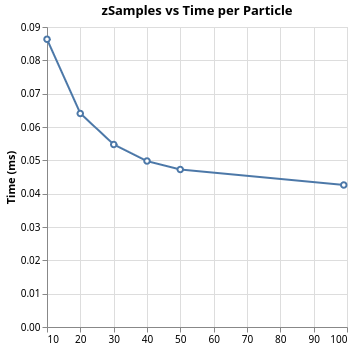
\includegraphics[scale=0.5]{Results/timeResultsZ/zSamplesTimePerParticle.png}
    \caption{Number of samples in the z direction vs computation time 
    spent per particle}
\end{figure}

\subsubsection{Experimenting with Rugosity Thresholds}

For our final test of the terrain decomposition, we reactivated the 
cell subdivision, and we experimented with different rugosity thresholds 
for subdivisions. First, we tested only performing one subdivision and changing 
the rugosity threshold (all rugosities are measured using a window 
size of $8$). The results of this experiment can be seen in figure 
\ref{fig:rugosityResults1}.


\begin{figure}
    \centering

    \subfigure[Bassiero terrain using a 151x138 grid. Subdivision performed 
    for cells with rugosity $> 1.5$]{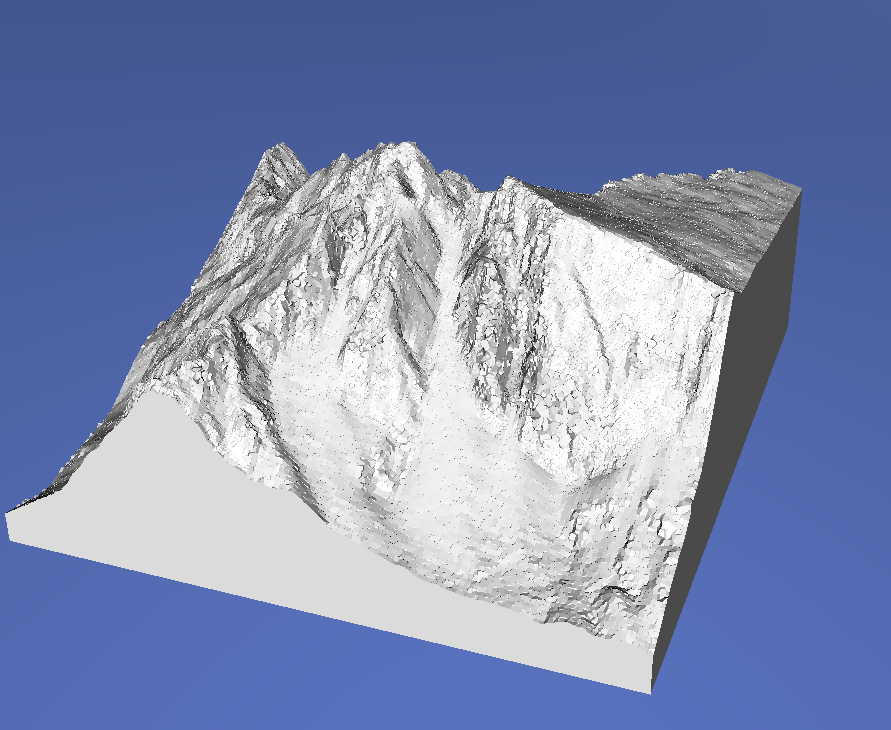
\includegraphics[width=0.3\linewidth]{Results/rugosityResults/division1.5.png}
    }
    \hspace{10pt}    
    \subfigure[Bassiero terrain using a 151x138 grid. Subdivision performed 
    for cells with rugosity $> 2.0$]{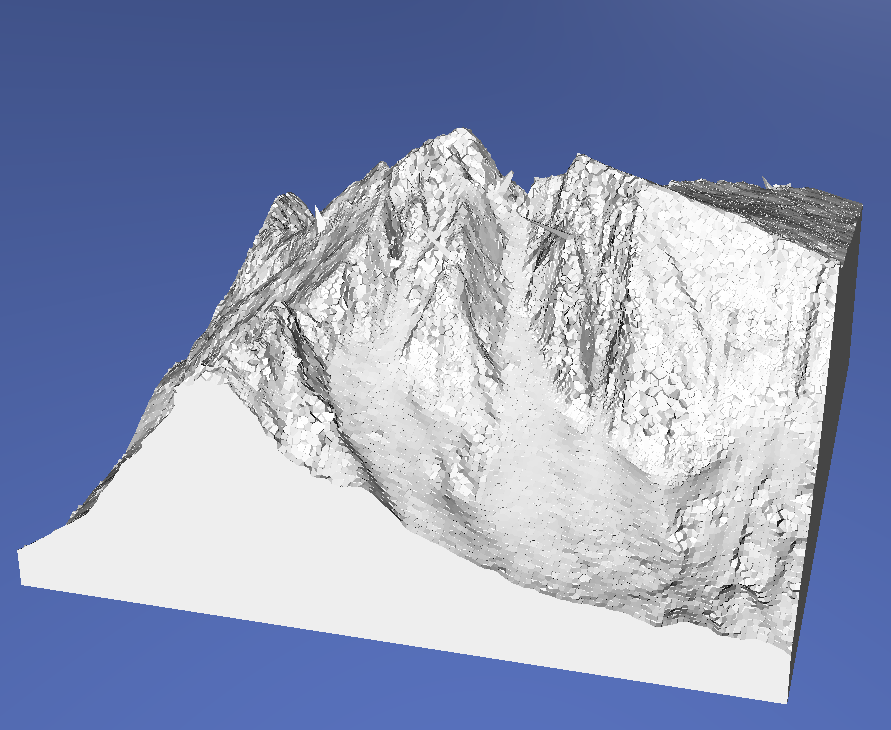
\includegraphics[width=0.3\linewidth]{Results/rugosityResults/divison2.0.png}}
    \hspace{10pt}
    \subfigure[Bassiero terrain using a 151x138 grid.Subdivision performed 
    for cells with rugosity $> 3.0$]{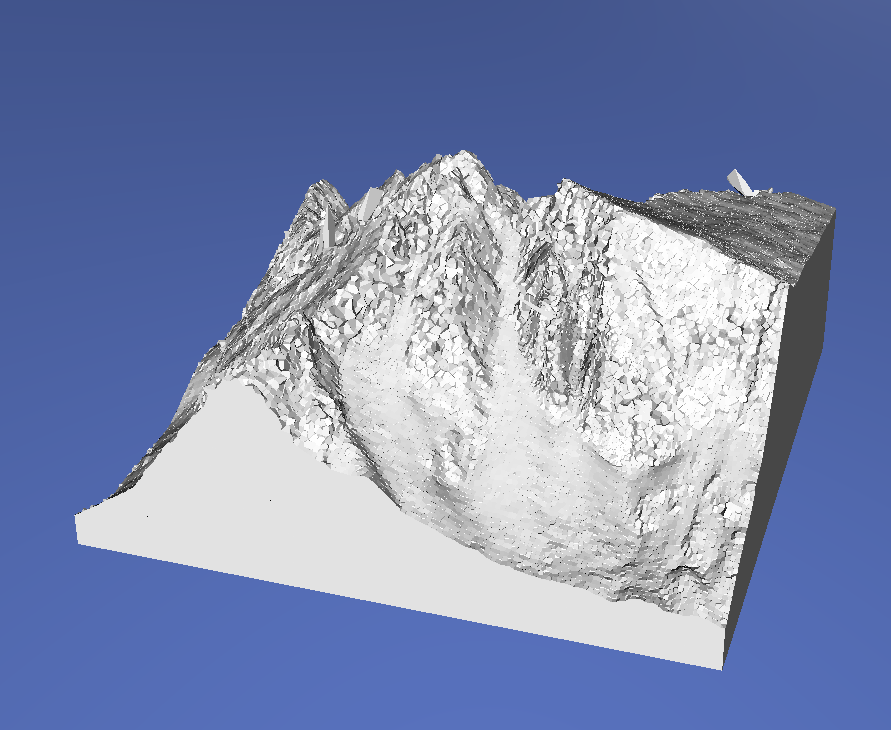
\includegraphics[width=0.3\linewidth]{Results/rugosityResults/division3.0.png}}

    \caption{Results of changing the rugosity threshold on the  
    Bassiero terrain} 
    \label{fig:rugosityResults1}
\end{figure}

\vspace{10pt}

Then, because we are not limited to subdividing a cell only once, we 
tried setting two or even three subdivision thresholds. This 
implies that we will collect $2 \cdot 4^k$ samples per cell at the surface, where 
$k$ is the number of thresholds surpassed on that specific cell. In this 
test we tried setting the threshold combinations $\{1.5,2.0\}$ (the one 
definitively implemented in the application), $\{2.0, 2.5\}$ and $\{1.5, 
2.0, 2.5\}$. There is a marked difference between the first and the 
second test, while the difference between the first and the last 
(which is the one with the highest quality) is more subtle and only appreciated 
in the sections with higher rugosity. 
\begin{figure}
    \centering

    \subfigure[Bassiero terrain using a 151x138 grid. Subdivision performed 
    for cells with rugosity $> 1.5$ and further subdivision for cells above $2.0$]{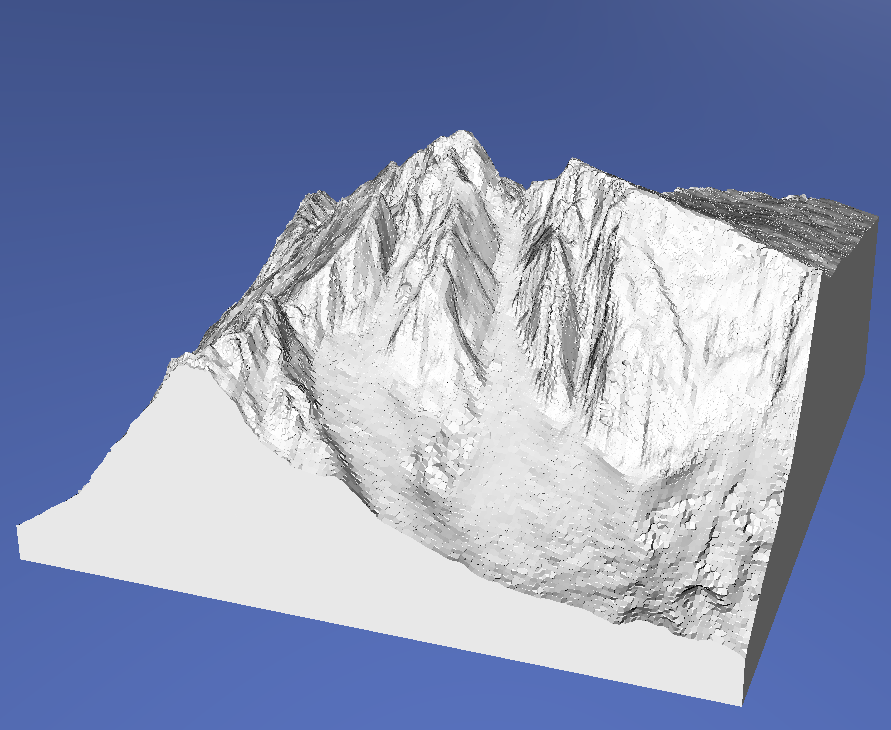
\includegraphics[width=0.3\linewidth]{Results/rugosityResults/division1.5_2.0.png}
    }
    \hspace{10pt}    
    \subfigure[Bassiero terrain using a 151x138 grid. Subdivision performed 
    for cells with rugosity $> 2.0$ and further subdivision for cells above $2.5$]{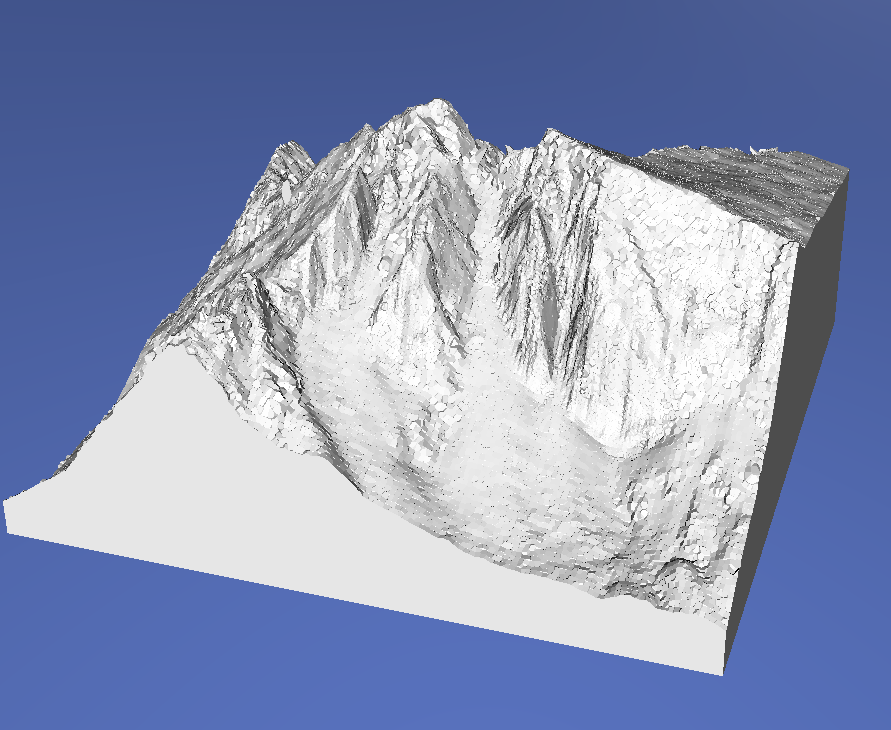
\includegraphics[width=0.3\linewidth]{Results/rugosityResults/division2.0_2.5.png}}
    \hspace{10pt}
    \subfigure[Bassiero terrain using a 151x138 grid.Subdivision performed 
    at three levels with thresholds $1.5$, $2.0$ and $2.5$]{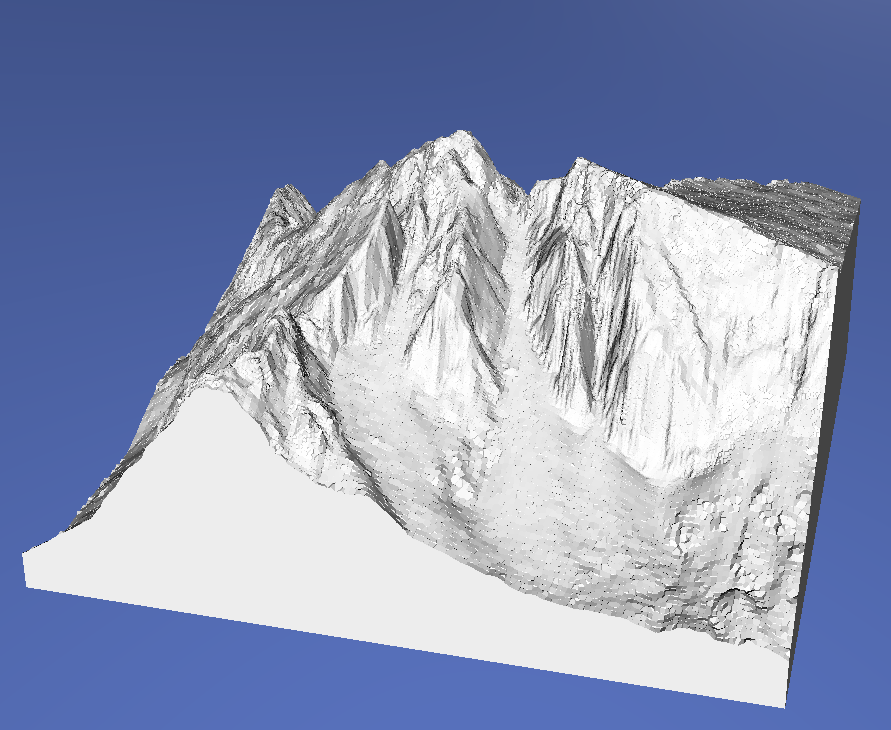
\includegraphics[width=0.3\linewidth]{Results/rugosityResults/division1.5_2.0_2.5.png}}

    \caption{Results of changing the rugosity threshold on the  
    Bassiero terrain. In this case, we performed further subdivisions 
    in cells where the rugosity is too high.} 
    \label{fig:rugosityResults2}
\end{figure}

\vspace{10pt}

Finally, we also measured the number of samples generated for every 
test, as well as its computation time. Table \ref{tab:rugosity} shows 
all measures we have taken for this batch of experiments. Remember 
that the computation time is not linear with respect to the number 
of particles, so it is important to choose a good balance between 
time spent and visual quality. In the final application, 
we decided to fix the threshold combination at $\{1.5, 2.0\}$, as 
we found that it provides a good balance.

\begin{table}[]
\centering
\begin{tabular}{|l|l|l|}
\hline
Thresholds             & Particles Generated & Time (s) \\ \hline
Base (No subdivisions) & 231713              & 12.639     \\ \hline
1.5                    & 293204              & 16.719     \\ \hline
2.0                    & 255445              & 14.180     \\ \hline
3.0                    & 233918              & 12.844     \\ \hline
1.5 \& 2.0              & 388023              & 22.715     \\ \hline
2.0 \& 2.5              & 285736              & 16.147     \\ \hline
1.5 \& 2.0 \& 2.5        & 509009              & 32.446     \\ \hline
\end{tabular}
\caption{Measures of our tests with different rugosity thresholds}
\label{tab:rugosity}
\end{table}

\subsubsection{Different Lighting Test}
The lighting method that we use highlights the borders between cells, 
as each face has a different normal. The lighting method chosen is 
useful to debug, but it can reduce the visual quality in some situations. 
As an experiment, we decided to reuse the same lighting method used to render 
the base heightfield (the one that the base application used) to 
properly compare the base model with its decomposition. Figure \ref{fig:lightingTest}
shows the results of this experiment: the terrain looks basically the 
same except for the walls (generated during the decomposition). It is 
important to note that this lighting method assigns a color based 
on the position of a point in the 2D grid of the DEM, so all points 
with the same $(x,y)$ coordinates will have the same color.

\begin{figure}
    \centering

    \subfigure[Base Aneto terrain]{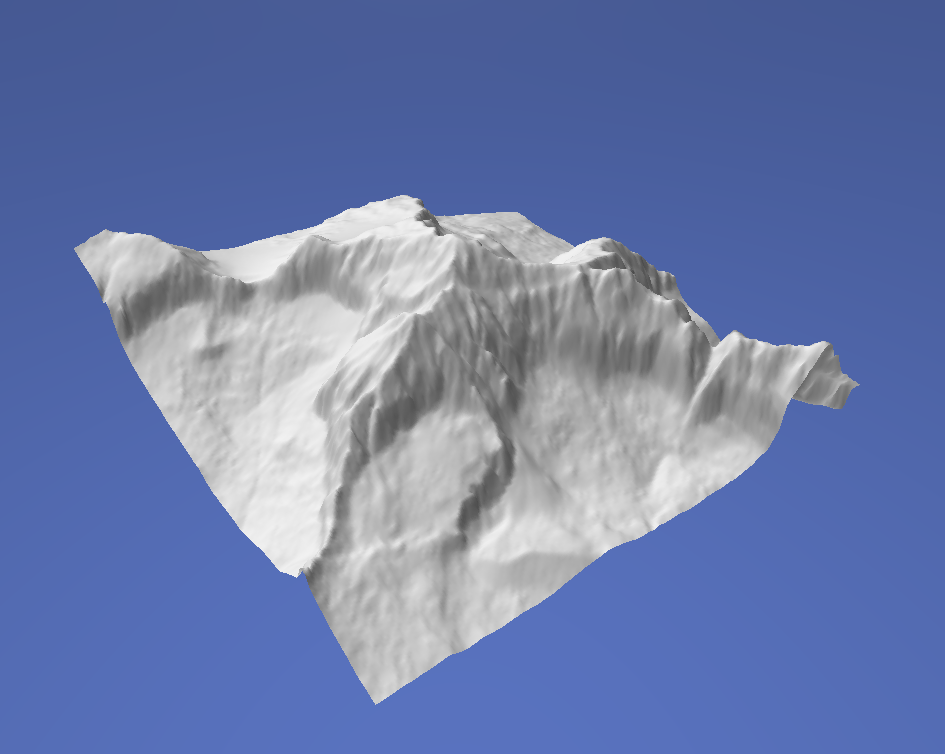
\includegraphics[width=0.4\linewidth]{Results/BaseAneto.png}
    }
    \hspace{20pt}    
    \subfigure[Aneto terrain after the decomposition]{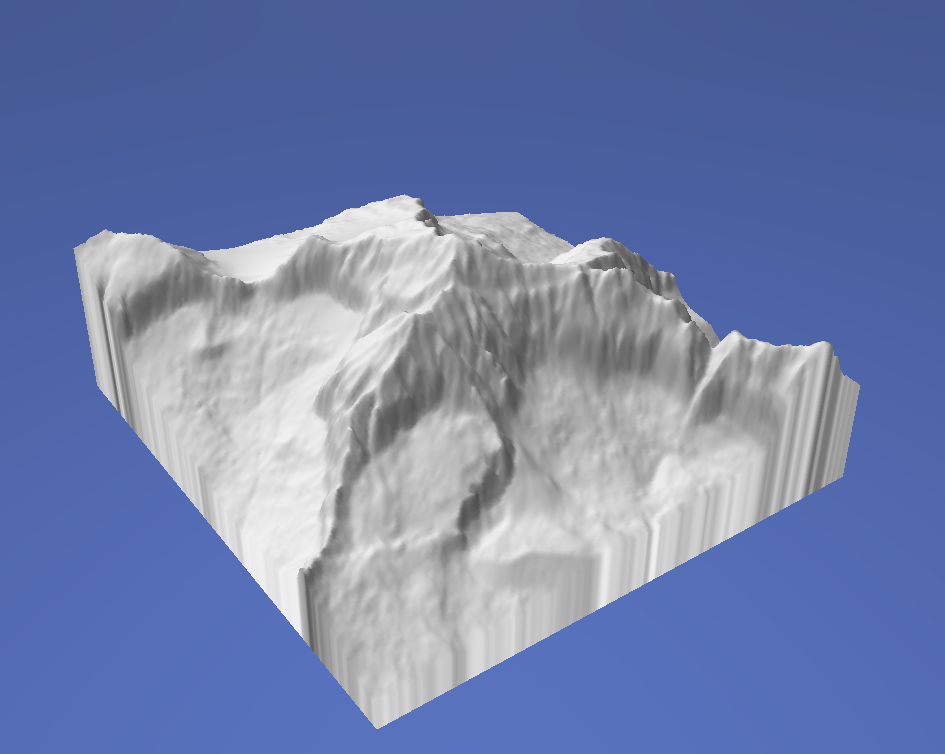
\includegraphics[width=0.4\linewidth]{Results/AnetoCells.png}}
  
    \caption{Comparison of the base terrain and the decomposition result using 
    the same lighting} 
    \label{fig:lightingTest}
\end{figure}

\subsection{Multi-Resolution Comparison}

In addition to the tests regarding the initial decomposition, we also 
compared our two proposed methods for subsampling. These two methods 
are hard to compare, as the method of subsampling in a grid does 
not allow for an easy manipulation of the total size of the subsampling 
(the grid that we use to sample and subsample is terrain dependent so 
we cannot know the exact size of the sampling). 
Despite these limitations, we decided to take some measures for each 
method in order to perform some comparisons. 

\vspace{10pt}

First, we tested both the time to compute and the final result of the 
furthest point sampling using $N/s$ subsamples where $s \in \{3,5,10,20\}$, 
and then, we tested the subsampling method based on a grid using 2x2x2, 
3x3x3, and 4x4x4 blocks of grid cells. The visual results can be appreciated 
in figures \ref{fig:furthestComparison} and \ref{fig:gridMultiRes}, and 
the computation time of each situation is written in table \ref{tab:subsamplingTable}.
All time measures are taken from the start of the decomposition to the 
completion of the low-resolution layer, so they all include the base time 
to produce the initial sampling. 

\vspace{10pt}

Even if these two methods are hard to compare, we can see that, 
with a similar amount of particles (using a downsampling factor of 
20 vs a 2x2x2 grid), the grid method is much more efficient in producing 
the computation and also produces shapes that more closely resemble 
the base terrain. Additionally, the examples that use the grid 
method add very little overhead over the initial sampling of the 
decomposition; if we subtracted the time of the initial computation 
to the total computation times, we would see a sharper difference 
between the furthest point and the grid methods. 

\begin{figure}
    \centering

    \subfigure[Bassiero terrain subsampled using furthest point with a downscale factor of $3$]{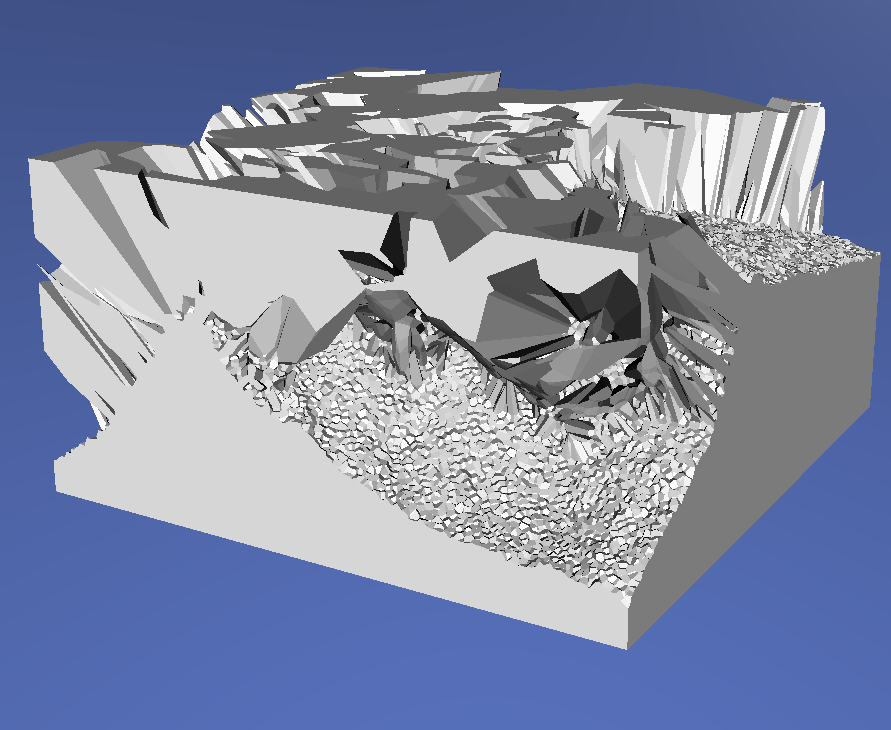
\includegraphics[width=0.3\linewidth]{Results/MultiResComparison/furthest3.png}
    }
    \hspace{10pt}    
    \subfigure[Bassiero terrain subsampled using furthest point with a downscale factor of $5$]{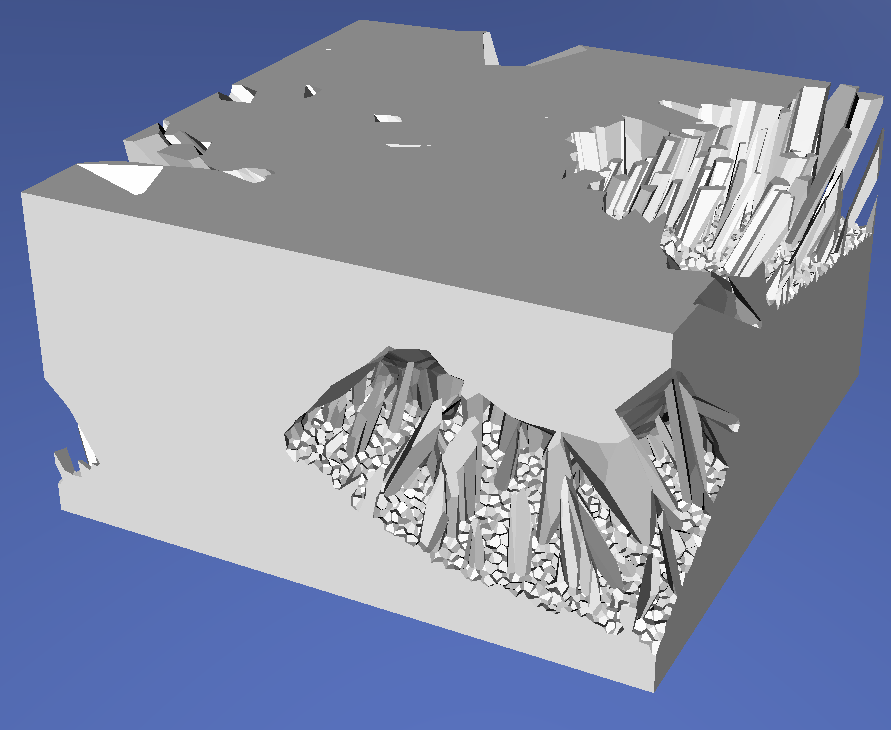
\includegraphics[width=0.3\linewidth]{Results/MultiResComparison/furthest5.png}}
    \hspace{10pt}
    \subfigure[Bassiero terrain subsampled using furthest point with a downscale factor of $10$]{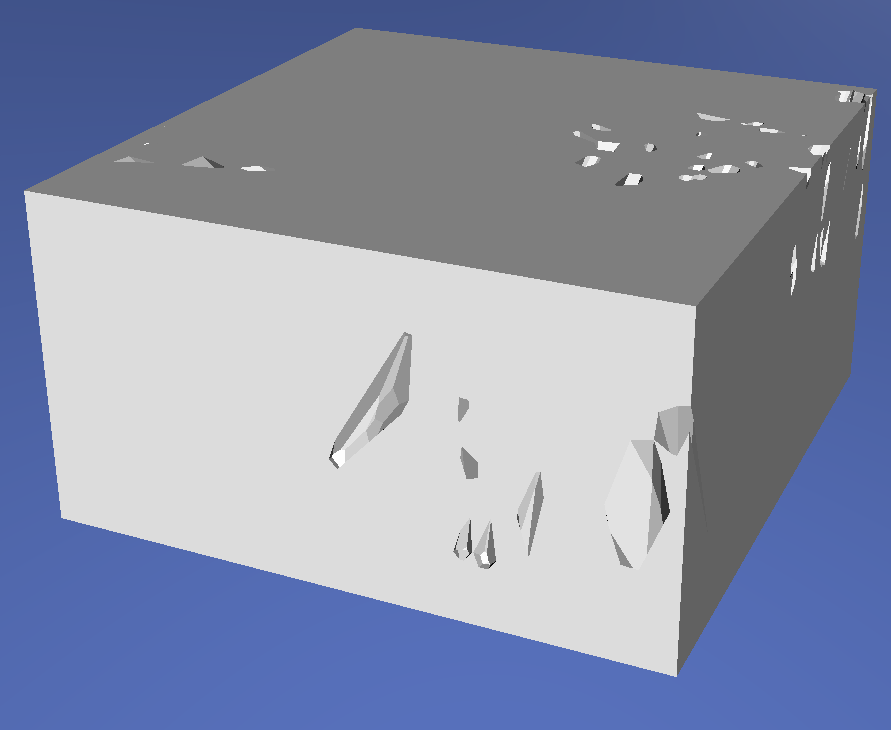
\includegraphics[width=0.3\linewidth]{Results/MultiResComparison/furthest10.png}}

    \caption{Different downscaling factors for the furthest point sampling method 
    applied to the \textit{Bassiero} terrain. 
    } 
    \label{fig:furthestComparison}
\end{figure}

\begin{figure}
    \centering

    \subfigure[Bassiero terrain subsampled using a subgrid made of 2x2x2 blocks]{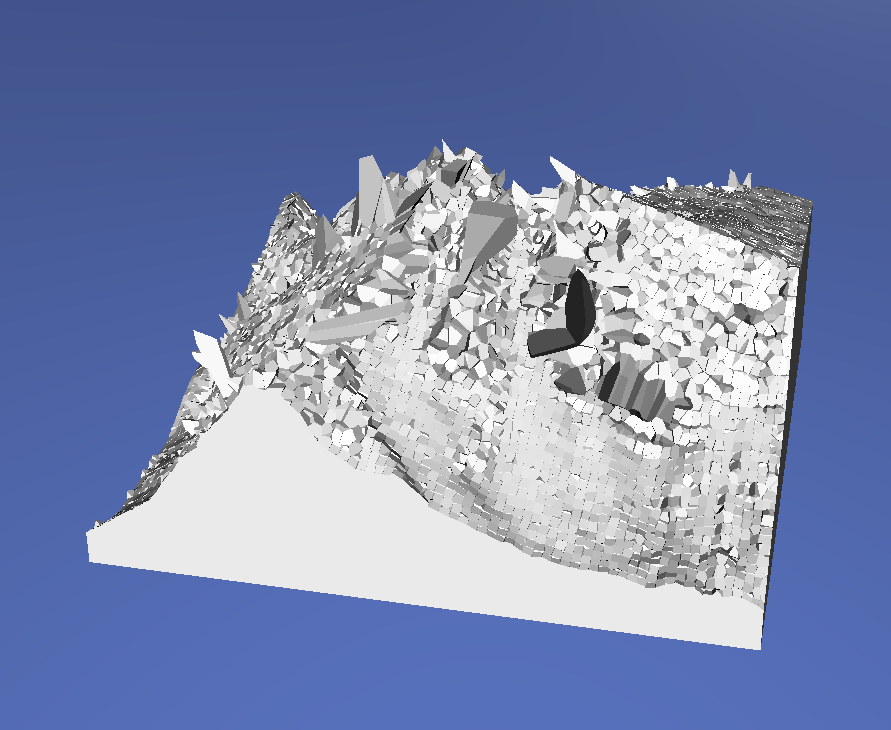
\includegraphics[width=0.3\linewidth]{Results/MultiResComparison/grid2x2.png}
    }
    \hspace{10pt}    
    \subfigure[Bassiero terrain subsampled using a subgrid made of 3x3x3 blocks]{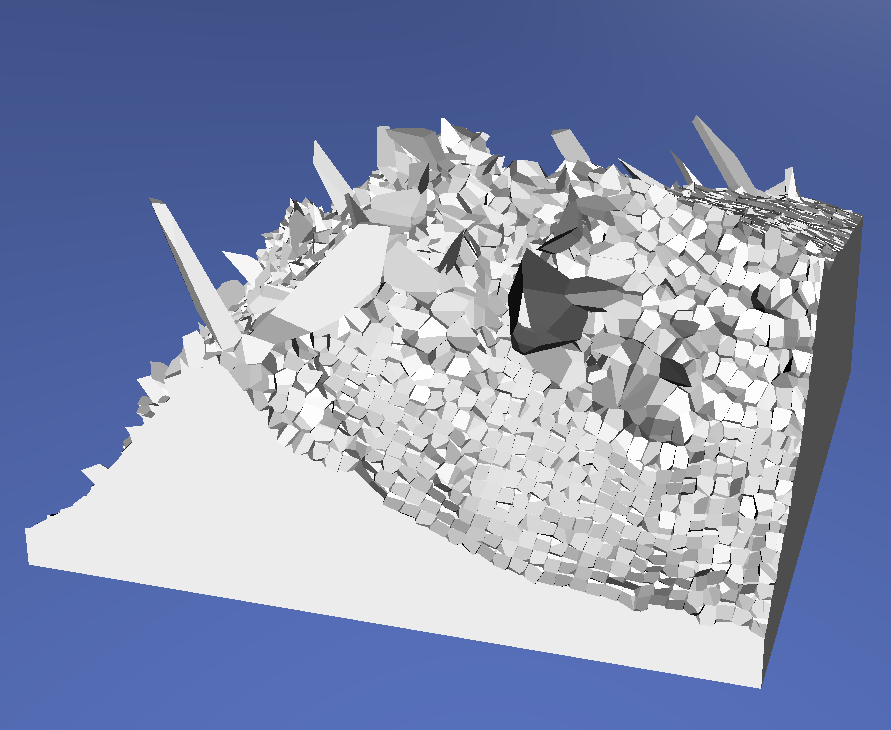
\includegraphics[width=0.3\linewidth]{Results/MultiResComparison/grid3x3.png}}
    \hspace{10pt}
    \subfigure[Bassiero terrain subsampled using a subgrid made of 4x4x4 blocks]{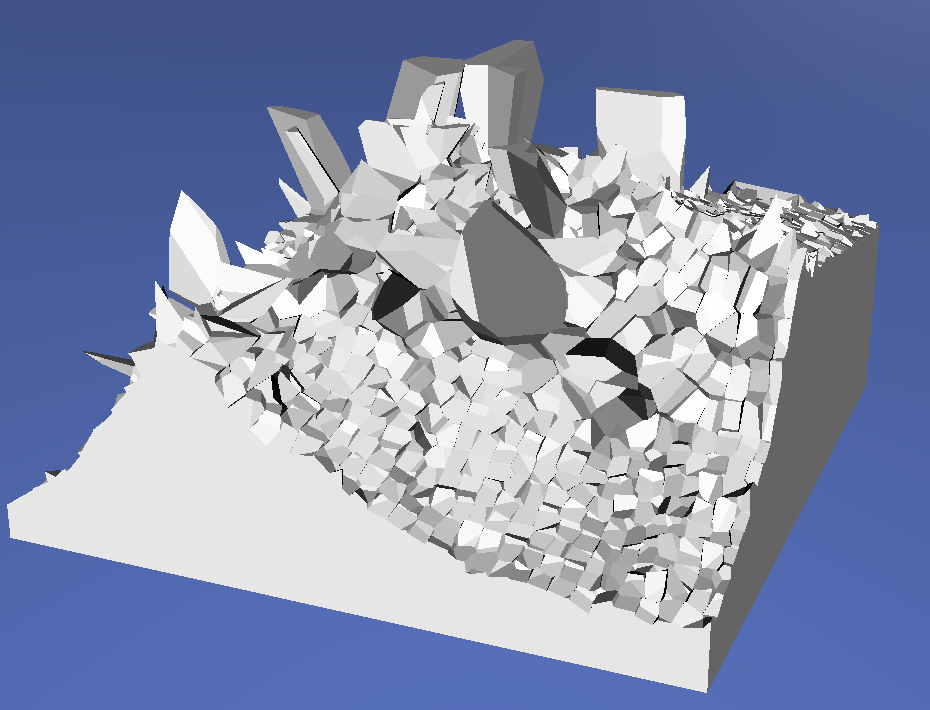
\includegraphics[width=0.3\linewidth]{Results/MultiResComparison/grid4x4.png}}

    \caption{Comparison of different block sizes used to make a subsampled gird. Applied to 
    the \textit{Bassiero} Terrain.} 
    \label{fig:gridMultiRes}
\end{figure}

\begin{table}[]
\centering

\begin{tabular}{|l|l|l|}
\hline
Multi-Resolution factor  & Particles Generated & Time (s) \\ \hline
Base (single resolution) & 411635              & 22.813     \\ \hline
Furthest Point: 3        & 137211              & 283.913    \\ \hline
Furthest Point: 5         & 82327               & 183.684    \\ \hline
Furthest Point: 10        & 41163               & 103.141    \\ \hline
Furthest Point: 20        & 20581               & 64.237     \\ \hline
Grid: 2x2x2              & 26208               & 25.673     \\ \hline
Grid: 3x3x3              & 10294               & 24.210     \\ \hline
Grid: 4x4x4              & 5398                & 23.775     \\ \hline
\end{tabular}
\caption{Comparison between the two subsampling methods that we implemented}
\label{tab:subsamplingTable}
\end{table}



\section{Erosion Simulation}
In this project we deeply tested the erosion simulation algorithm, trying 
different paramaters and different decompositions, comparing the old 
algorithm versus the new one. In this section we are going to go over 
our implementation of the erosion process as well as explain all our 
findings from our experiments.

\subsection{UI For Erosion}
Before explaining our findings, we are going to show how the user can 
control the different aspects of the simulation. Most parameters, 
like the material properties are set in the \textit{mechanicalModel.h} 
header with no option to control them on the UI, but the user still 
has some freedom using just the UI.

\subsubsection{Erosion Menu}

From the erosion menu of the UI (shown in figure \ref{fig:erosionMenu}), the 
user can modify the direction of water infiltration (as explained in section
\ref{sec:waterPaths}) and whether the mechanical model is used or not 
(keep in mind that an initial stress computation will be performed 
every time you activate the mechanical model option). 
Even if the user decides to not use the mechanical model, the button 
\textit{Compute Stresses} computes all stresses of the system and removes 
the links meeting the failure conditions; this way, we can simulate the 
process without the mechanical model up to a point and then compute all 
stresses of the system in that state. 

\vspace{10pt}

Finally, the user will have to select the number of paths to be generated 
simultaneously and press the button \textit{Compute Water Paths} to 
start the simulation.  
\begin{figure}
    \centering
    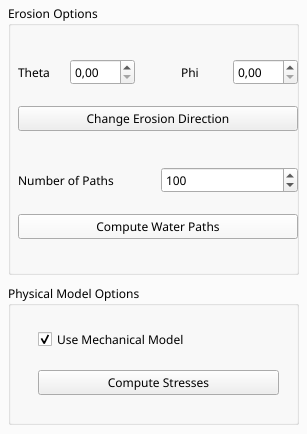
\includegraphics[scale=0.45]{Results/erosionMenu.png}
    \caption{Erosion menu of the UI}
    \label{fig:erosionMenu}
\end{figure}
\subsubsection{Visualization Options}
In addition to the simulation control options, the 
visualization menu \ref{fig:vorovisuals} also contains two options 
that are useful to debug the erosion process. First, we can visualize
the life of the links and their shear and normal stresses using 
the \textit{Render Links} option (figure \ref{fig:linkVisualization}), 
and second, we can paint blue the cells touched by the last batch of 
water paths (remember that the size of the batch is controlled using the 
erosion options), as shown in figure \ref{fig:waterPaths}.

\begin{figure}
    \centering

    \subfigure[Link life visualization. From Green (full life) to red (fully damaged)]{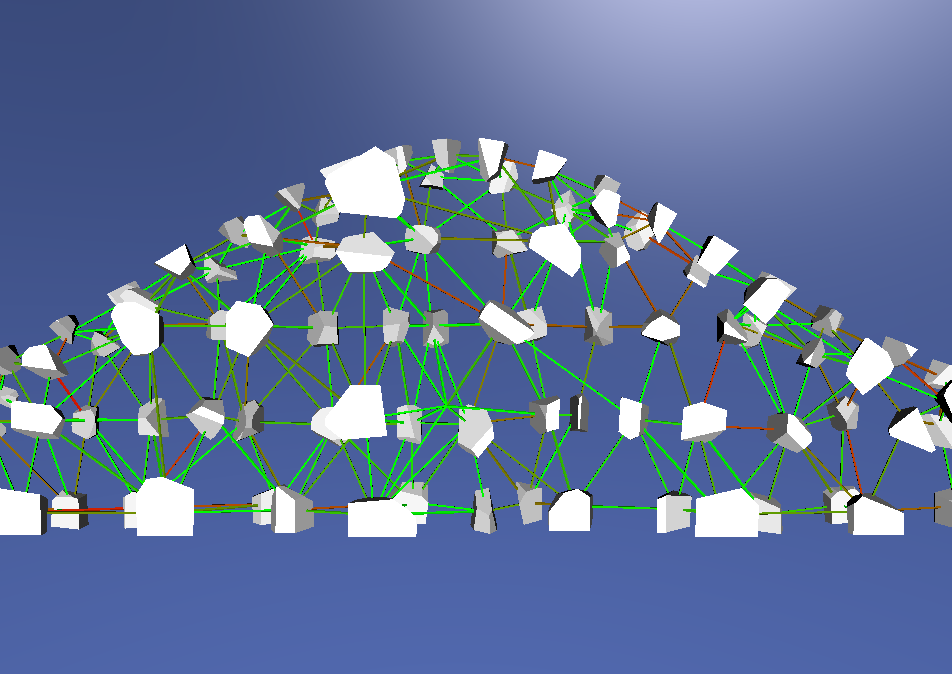
\includegraphics[width=0.278\linewidth]{Results/linkLife.png}
    }
    \hspace{10pt}    
    \subfigure[Link normal stress visualization. From blue to green for negative 
    normal stress (compression) and green to red for tension]{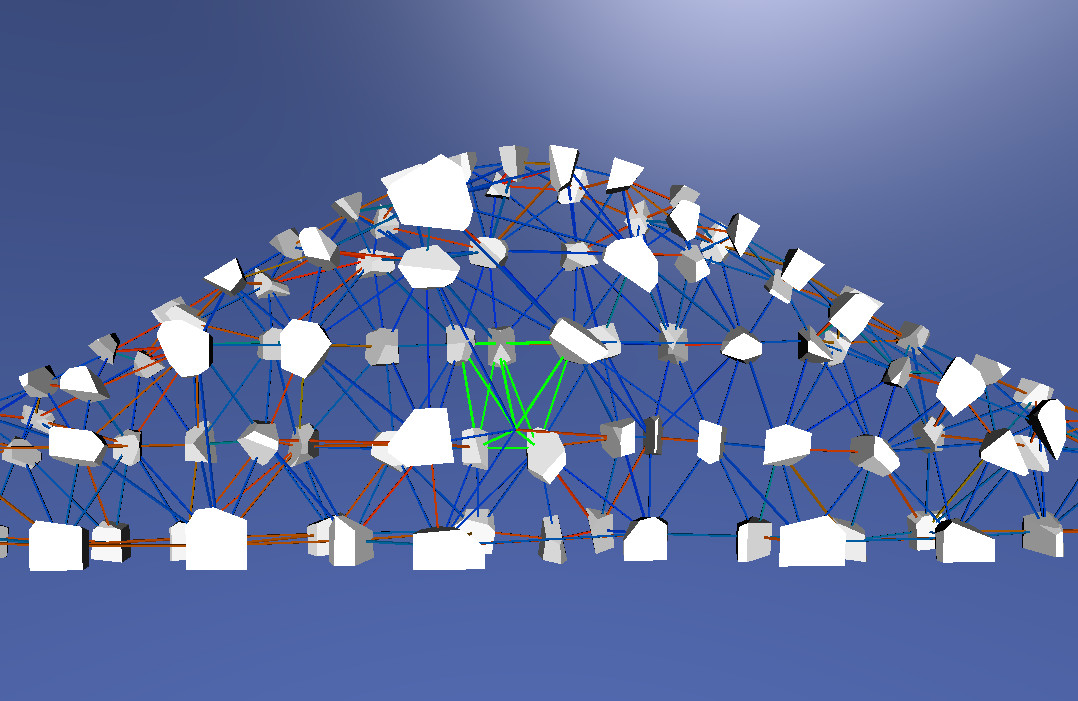
\includegraphics[width=0.3\linewidth]{Results/linkNormalStress.png}}
    \hspace{10pt}
    \subfigure[Link shear stress visualization. From green (0 stress) to red]{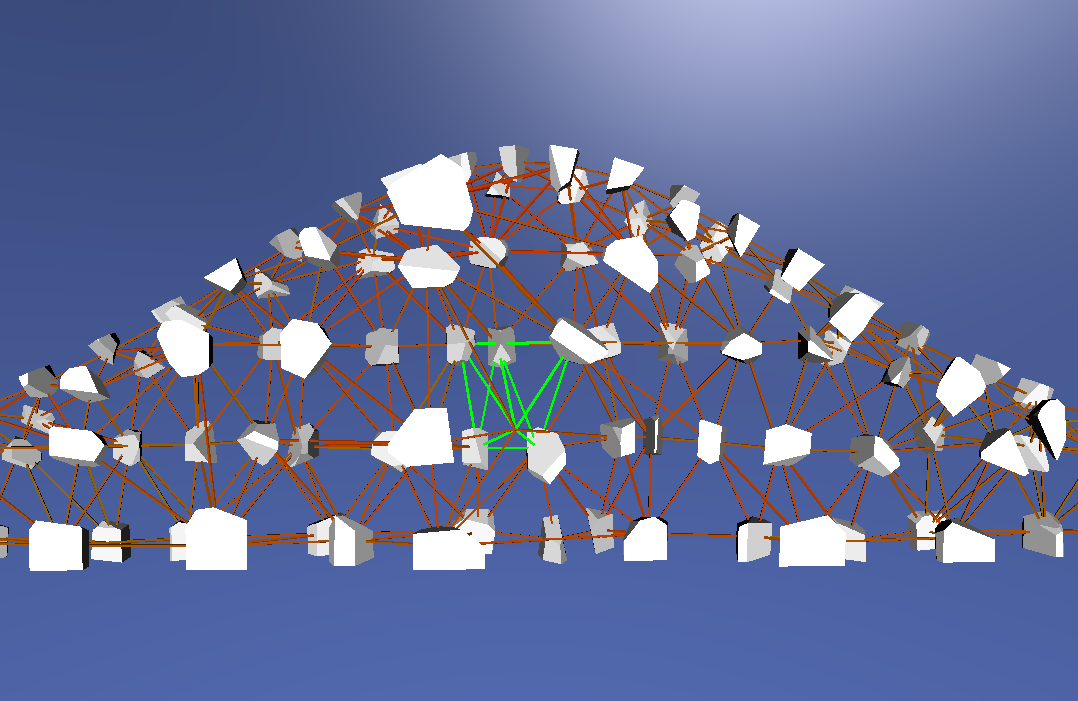
\includegraphics[width=0.3\linewidth]{Results/linkShearStres.png}}

    \caption{Different link visualization options} 
    \label{fig:linkVisualization}
\end{figure}

\begin{figure}
    \centering
    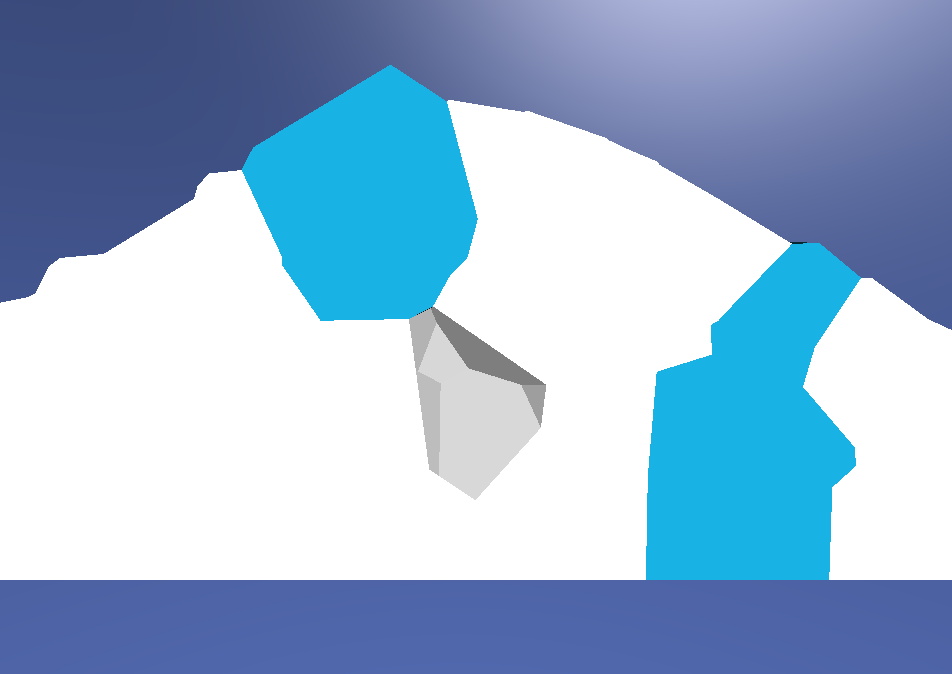
\includegraphics[scale=0.15]{Results/waterPaths.png}
    \caption{Simulation of 10 water paths on the \textit{Gaussian Bump}
    toy example. Cells that are touched by the water are painted in blue}
    \label{fig:waterPaths}
\end{figure}
\subsection{Base Algorithm Experimentation}
The first experiments that we conducted were all centered on 
the base algorithm as designed in \cite{10.2312:ceig.20241139}, without the inclusion of the mechanical model.
Having a set of experiments on the base method allows us to better 
compare both techniques and pinpoint the advantages of adding 
the mechanical model on top of the base one. 

\vspace{10pt}

Our first batch of experiments consited in comparing both 
implemented multi-resolution methods to check the difference 
in results and, additionally take measures of computational time. For 
these experiments, we tested 5 consecutive rounds of 10,000 paths for 
each multi-resolution method using the terrain \textit{Aneto} with 
resolution 197x199, and then 
3 consecutive rounds of 100,000 paths on a fresh instance of the 
same terrain. We decided to take multiple rounds of paths instead 
of just one single round with the combined number of paths to observe 
the evolution of the terrain step by step and check the influence 
of the current state of the terrain on the computational cost.

\vspace{10pt}

Regarding the final results, figure \ref{fig:100K Comparison} shows 
the base Aneto terrain compared against the result of simulating 
300 thousand water paths on each multi-resolution method. The 
furthest point method generated more cells than the grid method 
(66491 vs 18736), so a slower erosion process was expected. Still, 
as we mentioned in section \ref{sec:multiResolution}, the furthest 
point method has to consider some cells outside of the terrain 
as solid; this means that in order to start appreciating results on 
the terrain, we will have to wait for the outside cells to be removed, 
which makes the full simulation slower. 

\vspace{10pt}

In terms of the computational cost, we have seen that it increased 
for every consecutive round of 10,000 paths with both subsampling 
methods (figure \ref{fig:10KTime}). We think that the more damaged the 
links are, the more removal events will be triggered, which are the 
most computationally expensive procedures of the algorithm, so the total 
computation time will increase. Additionally, the more eroded the 
terrain is and the fewer cells remaining, the faster the algorithm 
should run, as the size of the problem becomes smaller. Following this logic, 
there should be a threshold where the cost of each consecutive round 
starts decreasing instead of increasing, as the size of the terrain 
starts getting significantly smaller.
Figure \ref{fig:100KTime} 
seems to confirm this idea, as the computational cost 
of the 100,000 path rounds decreases for each consecutive run 
in the grid method case. In the case of the furthest point sampling, 
we have already seen that the erosion process is slower, so we think 
that 300 thousand paths were not enough to reach the threshold where 
the time starts decreasing instead of increasing.


\begin{figure}
    \centering

    \subfigure[Aneto terrain before any erosion process]{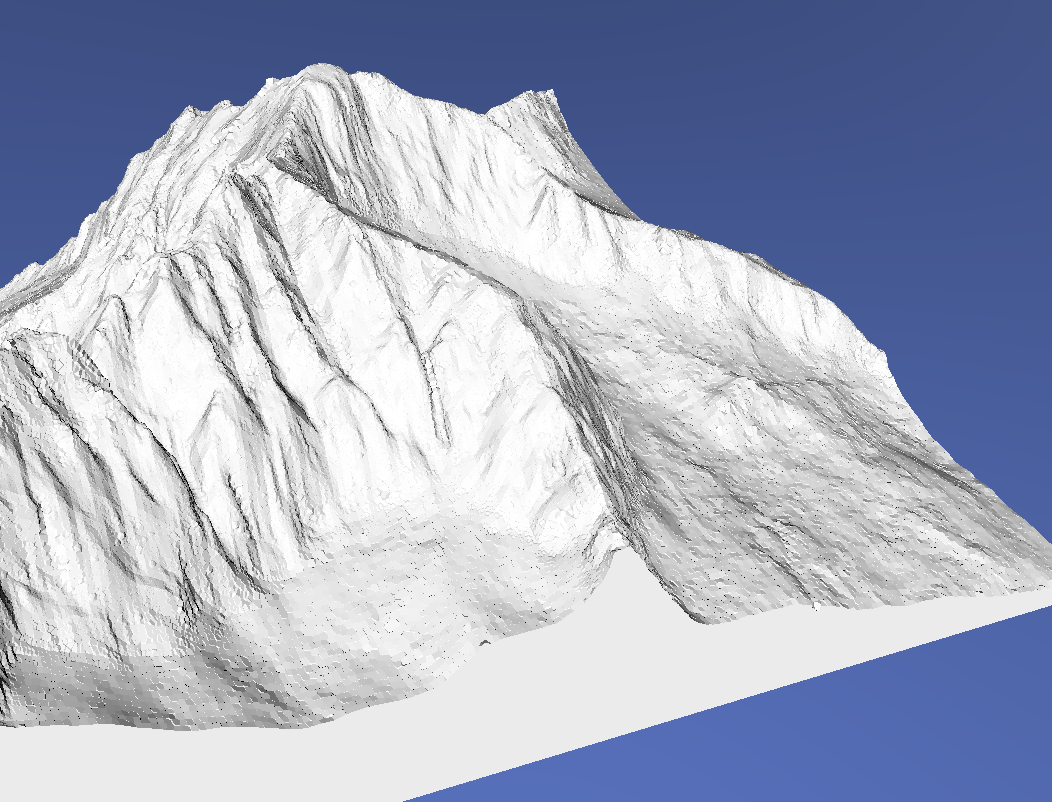
\includegraphics[width=0.3\linewidth]{Results/AnetoBefore300k.png}
    }
    \hspace{10pt}    
    \subfigure[Aneto terrain after 300 thousand paths using the furthest point method to subsample]{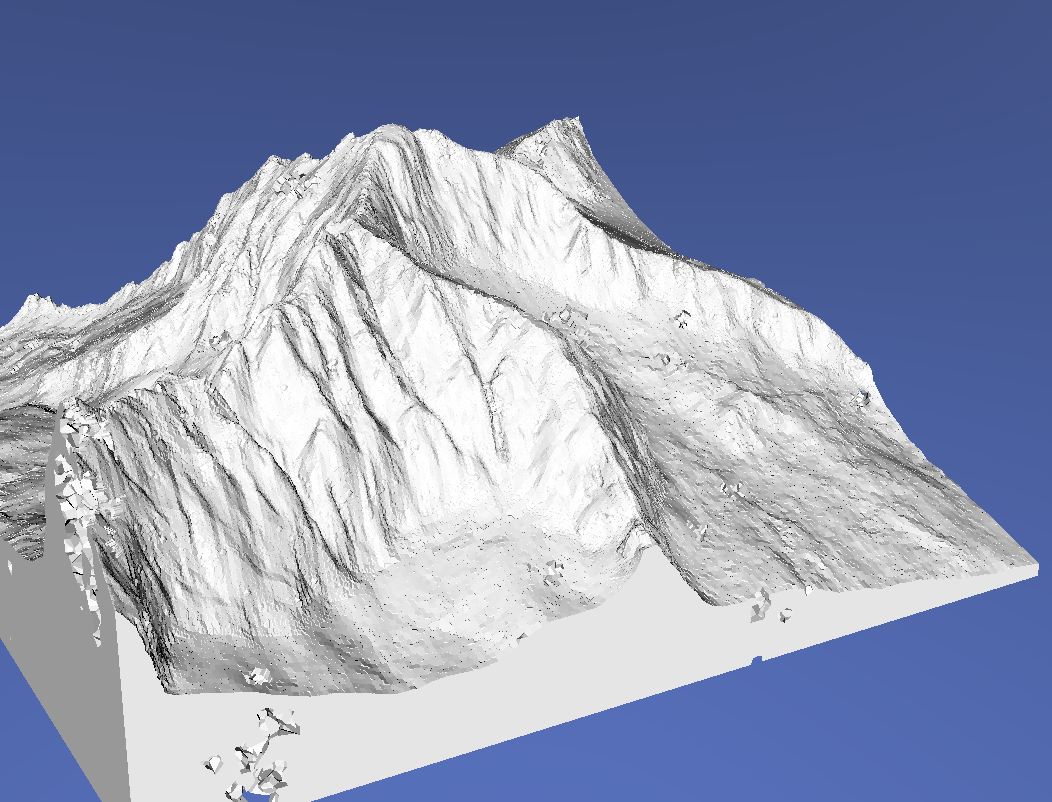
\includegraphics[width=0.3\linewidth]{Results/Aneto300K_general.png}}
    \hspace{10pt}
    \subfigure[Aneto terrain after 300 thousand paths using the grid method to subsample]{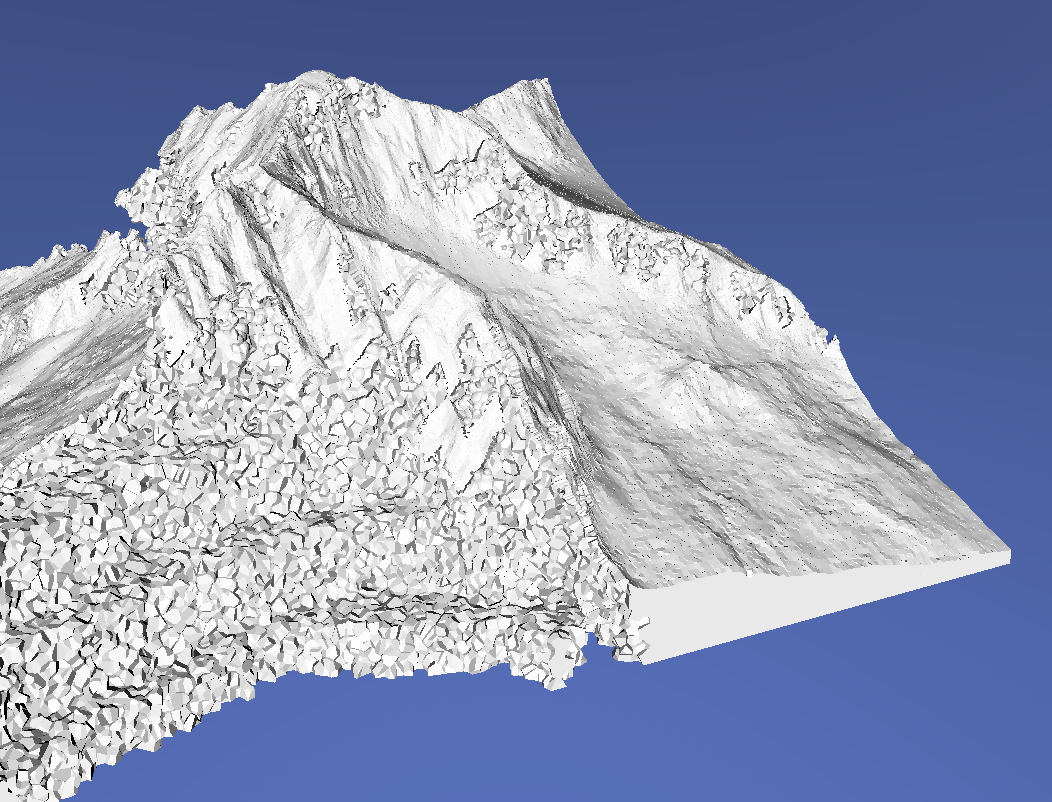
\includegraphics[width=0.3\linewidth]{Results/AnetoAfter300k.png}}

    \caption{Result of 300 thousand water paths on the Aneto terrain using different 
    subsampling methods to create the low-resolution decomposition} 
    \label{fig:100K Comparison}
\end{figure}

\begin{figure}
    \centering

    \subfigure[Time to complete different runs of 10K paths. The runs have been 
    executed one after the other on the same model]{\label{fig:10KTime}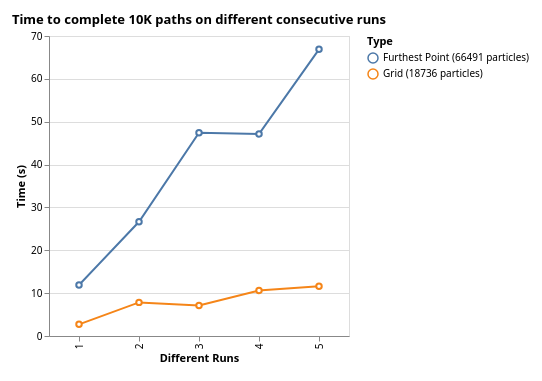
\includegraphics[width=0.4\linewidth]{Results/10KTime.png}
    }
    \hspace{20pt}    
    \subfigure[Time to complete different runs of 100K paths. The runs have been 
    executed one after the other on the same model]{\label{fig:100KTime}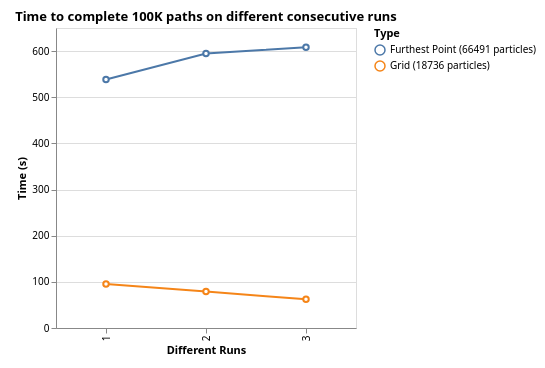
\includegraphics[width=0.41\linewidth]{Results/100KTime.png}}

    \caption{Time to complete of different consecutive runs with 10K 
    and 100K paths for run} 
    \label{fig:timeTestsBase}
\end{figure}

\subsubsection{Impact of Multi-Resolution in Computational Cost}

We have tested the base erosion algorithm applied on different 
multi-resolution methods, but we have not yet applied it 
to the high-resolution method without any kind of multi-resolution. 
During some test runs, we found that repeating an experiment 
like the one we just presented (running 100 thousand paths three times)
would be incredibly slow, so we decided to present two simpler comparisons 
to show the advantage of using the multi-resolution process. 

\vspace{10pt}

In the first experiment, we compared the results of the furthest point 
method with a downscale factor of 10 against the high-resolution using 
the terrain \textit{Aneto} with a resolution of 150x150 (the previously used 
197x199 resolution was too expensive), both executing 
100,000 paths. The furthest point method took 437 seconds (7 minutes and 17 seconds), 
while the high-resolution model took 1661 seconds (27 minutes and 41 seconds). 
Regarding the final results, the high-resolution terrain produced almost negligible 
erosion effects on the terrain, which implies that even more water paths 
are required to properly display erosion effects. These visual results 
can be seen in figure \ref{fig:highResVsLow}.

\vspace{10pt}

\begin{figure}
    \centering

    \subfigure[Results of 100,000 paths using the furthest point method for multi-resolution]{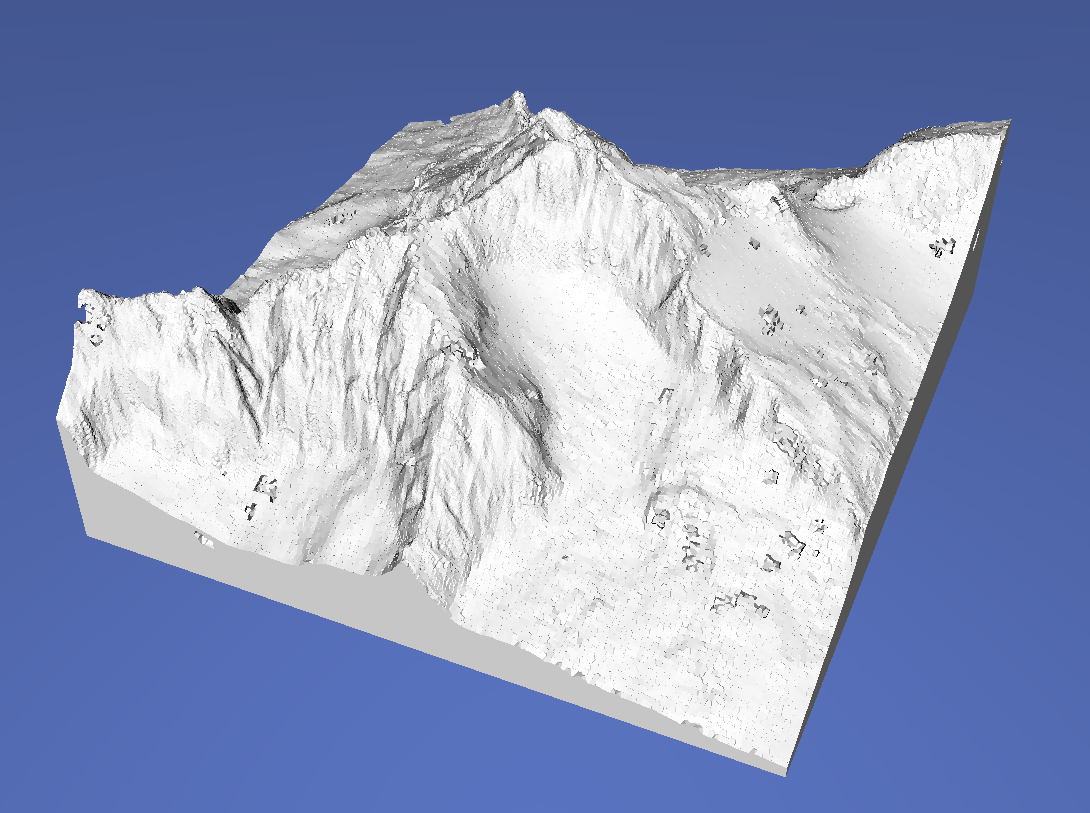
\includegraphics[width=0.38\linewidth]{Results/100KpathsAneto.png}
    }
    \hspace{20pt}    
    \subfigure[Results of 100,000 paths directly on the high resolution terrain]{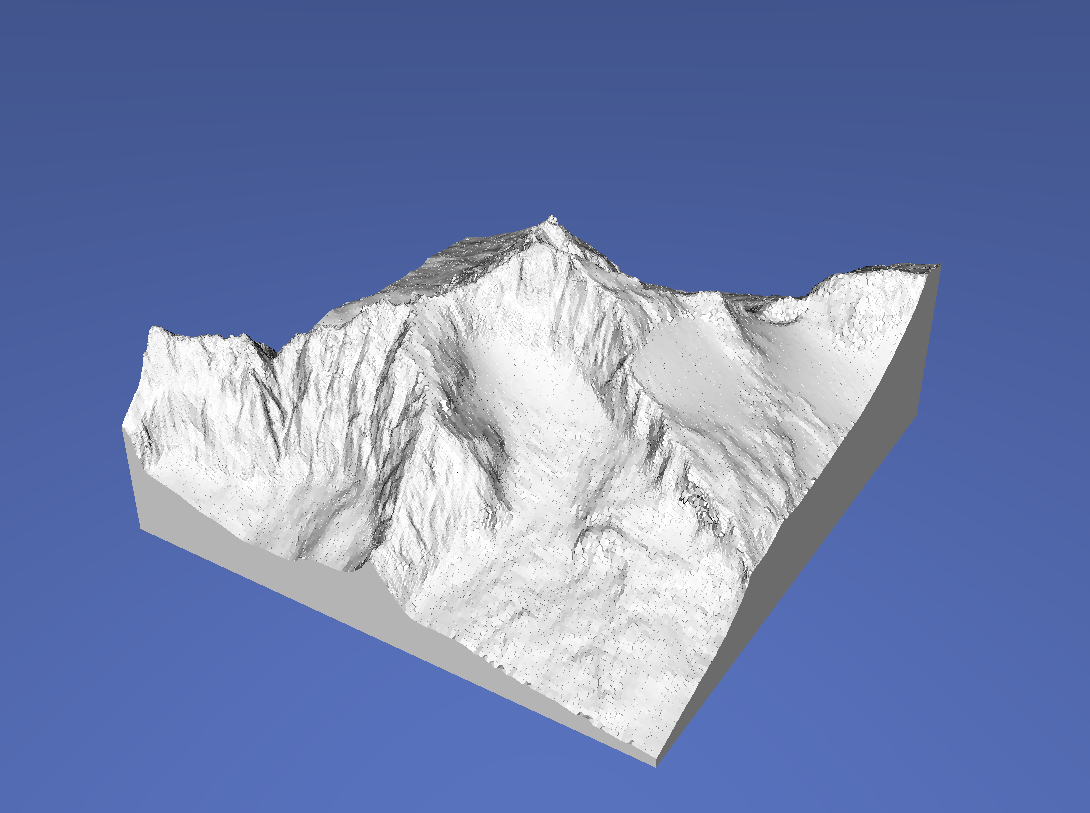
\includegraphics[width=0.38\linewidth]{Results/100KpathsAnetoHighres.png}}

    \caption{Results of 100,000 paths of the erosion simulation. Using a multi-resolution method 
    versus using the high resolution directly} 
    \label{fig:highResVsLow}
\end{figure}

The time that we save on the base erosion algorithm is highly significant, 
but having a multi-resolution method is even more essential if we want to use our 
mechanical model, as the difference is even greater. In order to show 
this difference, we initially wanted to test a single path 
in the high-resolution model using the same terrain we used for other 
experiments of the mechanical model (Aneto 50x50). We thought that a single 
path would show a huge difference in computation time, demonstrating 
the necessity for a multi-resolution method, but we could not even complete 
a single path (we timed out the experiment after an hour). This 
failure demonstrates the necessity of applying the multi-resolution method.

\vspace{10pt}

Despite this failure, we wanted to have some data to compare, so we tried 
again with a 25x25 Aneto terrain. In this case, the method that used 
multi-resolution took 587 ms for a single path, while the high-resolution 
model took 468149 ms (roughly 7 minutes and 48 seconds). This implies 
three orders of magnitude of difference between the two methods, and 
it seems to get even wider for higher terrain dimensions.
Using directly the high resolution for our tests would be basically 
unfeasible, so we completely discarded the idea of performing 
any comparison for other experiments.


\subsection{Mechanical Model Experimentation}
After experimenting with the base method, we are ready to test 
the algorithm using the mechanical model. The mechanical model is 
much more computationally expensive than the base algorithm due to the 
constant recomputation of the system of equations, so we need a simpler 
model to test. To perform all tests of our mechanical model, we used the \textit{Aneto} terrain with heightfield dimensions of
50x50 and a grid of 3x3x3 blocks for the low-resolution subsampling.

\subsubsection{Simulating Different Materials}

The number of parameters influencing our mechanical model is huge, and 
independently trying to tune every single one of them would be a challenging 
task. For that reason, we decided to first look in nature and try the 
mechanical properties of different rocks. We do not really need 
the parameters to exactly match the real ones, and we can work with 
an approximation, so we took the data from the website \cite{MakeitFrom} 
that lists some of the material properties of different materials. However,
that website does not list cohesion (c) and the coefficient of internal 
friction ($\varphi$), so we checked for those properties in other 
parts of the literature, like \cite{article}, \cite{article2}, and \cite{app15137481}.

\vspace{10pt}

Using the collected data on material properties, we did a test run for granite
just to check whether the model runs properly or not. In the test run,
we found that most links were, initially, over the shear stress limit, 
producing an initial crack propagation effect that destroyed a huge portion
of the terrain before starting the first path. For that reason, we decided 
to multiply by 10 the cohesion of all materials, and then we tried another test run 
with granite. In the second test run, some links broke initially due to 
tension, and a few cells were separated, but the initial damage was minor.
To avoid this initial damage we decided to increase the tensile strength 
by around 50\% on all materials. Figure \ref{fig:initialShearTension} shows 
the results of these two test runs.

\begin{figure}
    \centering

    \subfigure[Results using the initial cohesion, without modification]{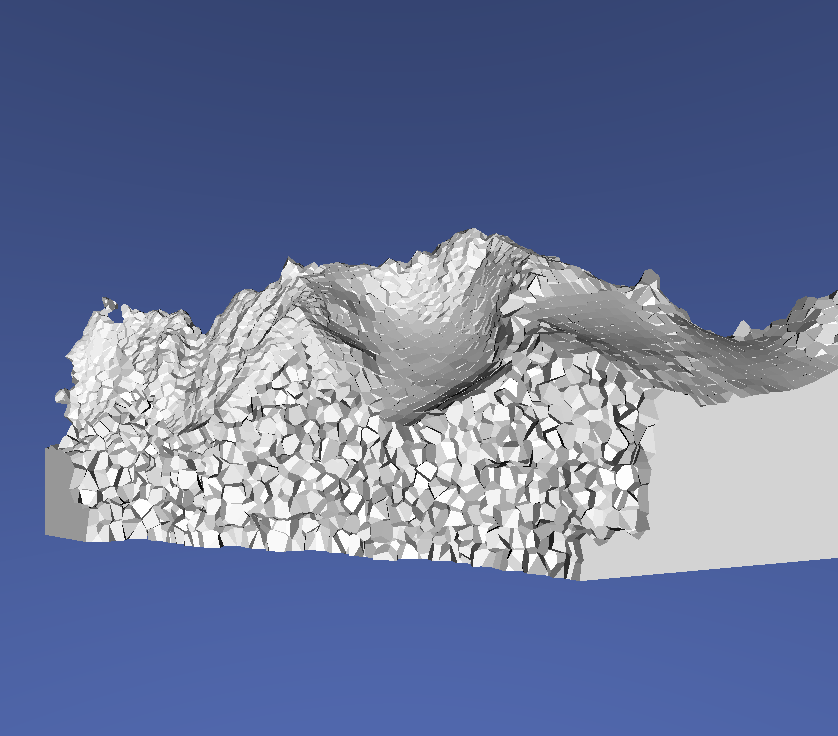
\includegraphics[width=0.38\linewidth]{Results/lowShearTest.png}
    }
    \hspace{20pt}    
    \subfigure[Minor damage initial damage on the terrain using the updated cohesion]{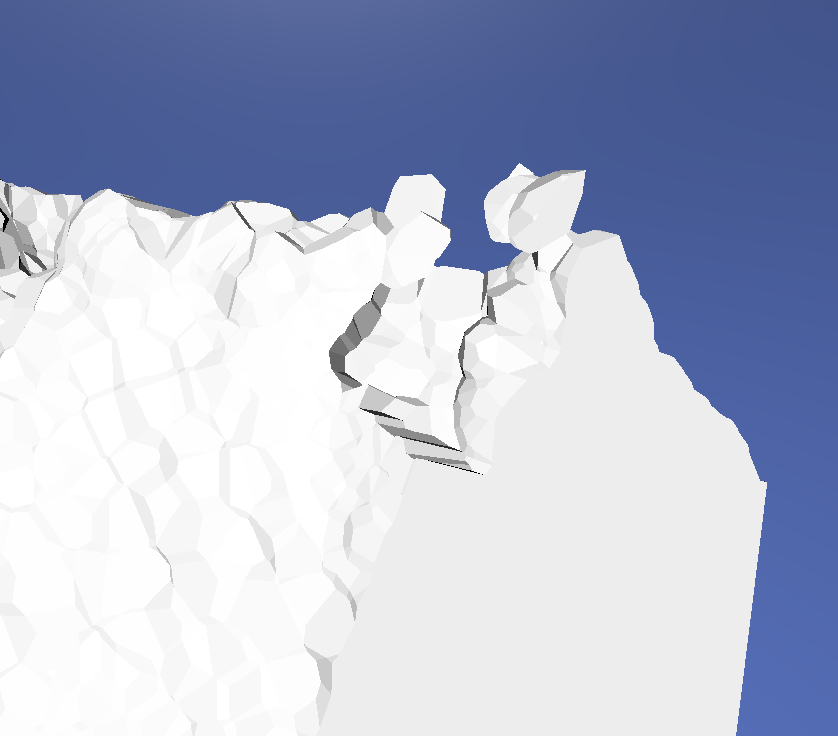
\includegraphics[width=0.38\linewidth]{Results/lowTensionTest.png}}

    \caption{Results of our test runs to tune the material properties} 
    \label{fig:initialShearTension}
\end{figure}

\vspace{10pt} 

\begin{table}[]
\centering
\begin{tabular}{|l|l|l|l|}
\hline
                             & Granite       & Marble        & Sandstone     \\ \hline
Density                      & $2650 \; kg/m^3$ & $2700 \; kg/m^3$ & $2600 \;  kg/m^3$ \\ \hline
Young's Modulus (E)          & 70 GPa          & 54 GPa          & 38 GPa          \\ \hline
Poisson's Ratio ($\upsilon$) & 0.255         & 0.2           & 0.25          \\ \hline
Tensile Strength ($T_{max}$)     & 60 MPa          & 12 MPa          & 6 MPa           \\ \hline
Compressive Strength (UCS)   & 2.2 GPa         & 540 MPa         & 120 MPa         \\ \hline
Cohesion (c)                 & 200 MPa         & 700 MPa         & 200 MPa         \\ \hline
$tan(\varphi)$                  & 0.267949      & 0.57735026    & 0.83909963   \\ \hline
\end{tabular}
\caption{Parameters of the tested materials. Some properties have 
been adjusted to our algorithm and might not fully represent the true 
material properties}
\label{tab:baseMaterialProperties}
\end{table}

After these test runs, we set the material properties of granite, marble, and 
sandstone to the values shown in table \ref{tab:baseMaterialProperties} and 
then started some experiments to compare the three. Granite showed 
pretty good results after simulating 100 paths (although we could not 
get to 200); the simulation took 
around 1000 seconds, and it produced a big hole in the middle of the 
mountain (somewhat resembling a volcano). Regarding the other two materials, 
marble showed some fractures after the initial stress computation (before 
generating any water path) and then completely collapsed after just 10 
paths, while sandstone did not even survive the initial stress computation. 
We based our parameters on the initial test runs on granite (which is 
the only one that survived a few paths), but it seems that our takeaways 
from the test runs were not really applicable to the other two materials.

\begin{figure}
    \centering

    \subfigure[Results of a granite Aneto after 100 water paths. 
    The terrain fully collapsed after just a few more paths]{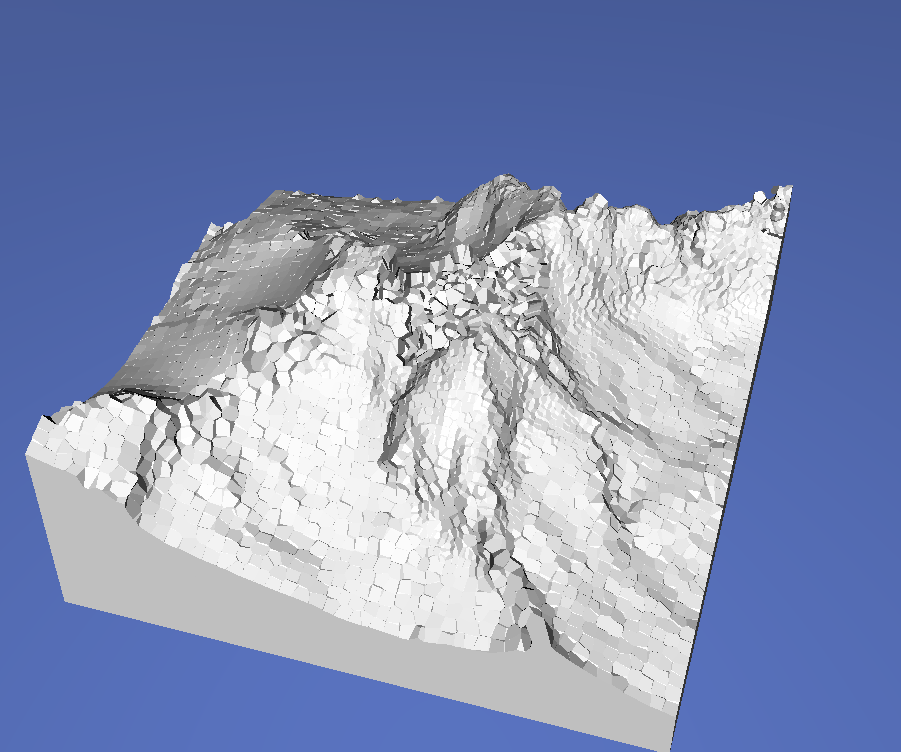
\includegraphics[width=0.4\linewidth]{Results/GraniteBase100.png}
    }
    \hspace{20pt}    
    \subfigure[Results of a marble Aneto after the initial stress computation (0 paths). The 
    terrain collapsed when we tried to simulate a few paths]{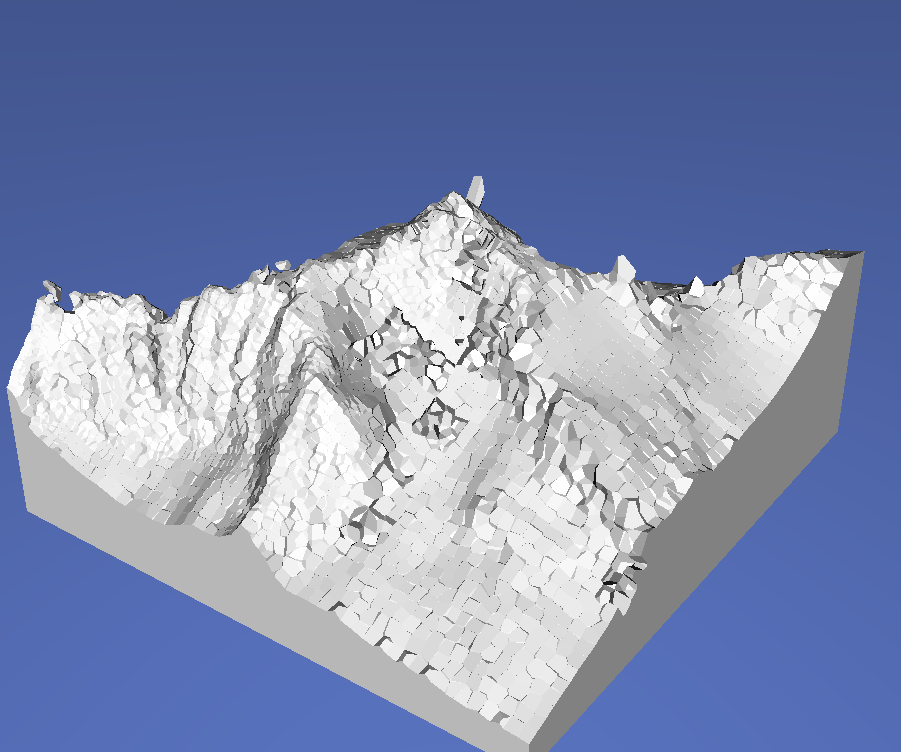
\includegraphics[width=0.4\linewidth]{Results/MarbleBase0.png}}

    \caption{Results of our experiments with different materials, just 
    before the terrains fully collapsed. Granite 
    sill retained some stability after 100 water paths, but marble collapsed 
    after less than 10} 
    \label{fig:initialMaterials}
\end{figure}

\subsubsection{Reinforced Materials}

In response to the poor results of the first experiments with different 
materials, we decided to reinforce their tensile strength so they 
can resist at least a few water paths. We decided to adjust 
just the tensile strength because most links were breaking due to tension 
and not due to shear or compression stresses. To differentiate these 
modified materials from the base materials that we tried previously, 
we decided to call them \textit{reinforced materials}, with properties 
shown in table \ref{tab:reinforcedMaterials}.


\begin{table}[]
\centering
\begin{tabular}{|l|l|l|l|}
\hline
                             & Reinforced Granite       & Reinforced Marble        & Reinforced Sandstone     \\ \hline
Density                      & $2650 \; kg/m^3$ & $2700 \; kg/m^3$ & $2600 \;  kg/m^3$ \\ \hline
Young's Modulus (E)          & 70 GPa          & 54 GPa          & 38 GPa          \\ \hline
Poisson's Ratio ($\upsilon$) & 0.255         & 0.2           & 0.25          \\ \hline
Tensile Strength ($T_{max}$)     & 390 MPa         & 120 MPa          & 60 MPa           \\ \hline
Compressive Strength (UCS)   & 2.2 GPa         & 540 MPa         & 120 MPa         \\ \hline
Cohesion (c)                 & 200 MPa         & 700 MPa         & 200 MPa         \\ \hline
$tan(\varphi)$                  & 0.267949      & 0.57735026    & 0.83909963   \\ \hline
\end{tabular}
\caption{Parameters that we used as our \textit{reinforced} materials}
\label{tab:reinforcedMaterials}
\end{table}

\vspace{10pt}

Using these new reinforced materials, our experiments looked much better, and 
we were able to compare the effect of changing the material on the 
overall results. After 400 water paths on each material, granite 
produced multiple holes but remaind fairly stable; sandstone had a wide 
portion completely destroyed; and, finally, 
marble seemed the most resistant, producing thin and shallow holes. 
The comparison between the different materials can be seen in figure \ref{fig:meterialComparison}

\begin{figure}
    \centering

    \subfigure[Eroion simulation after 400 paths on reinforced granite. Overview]{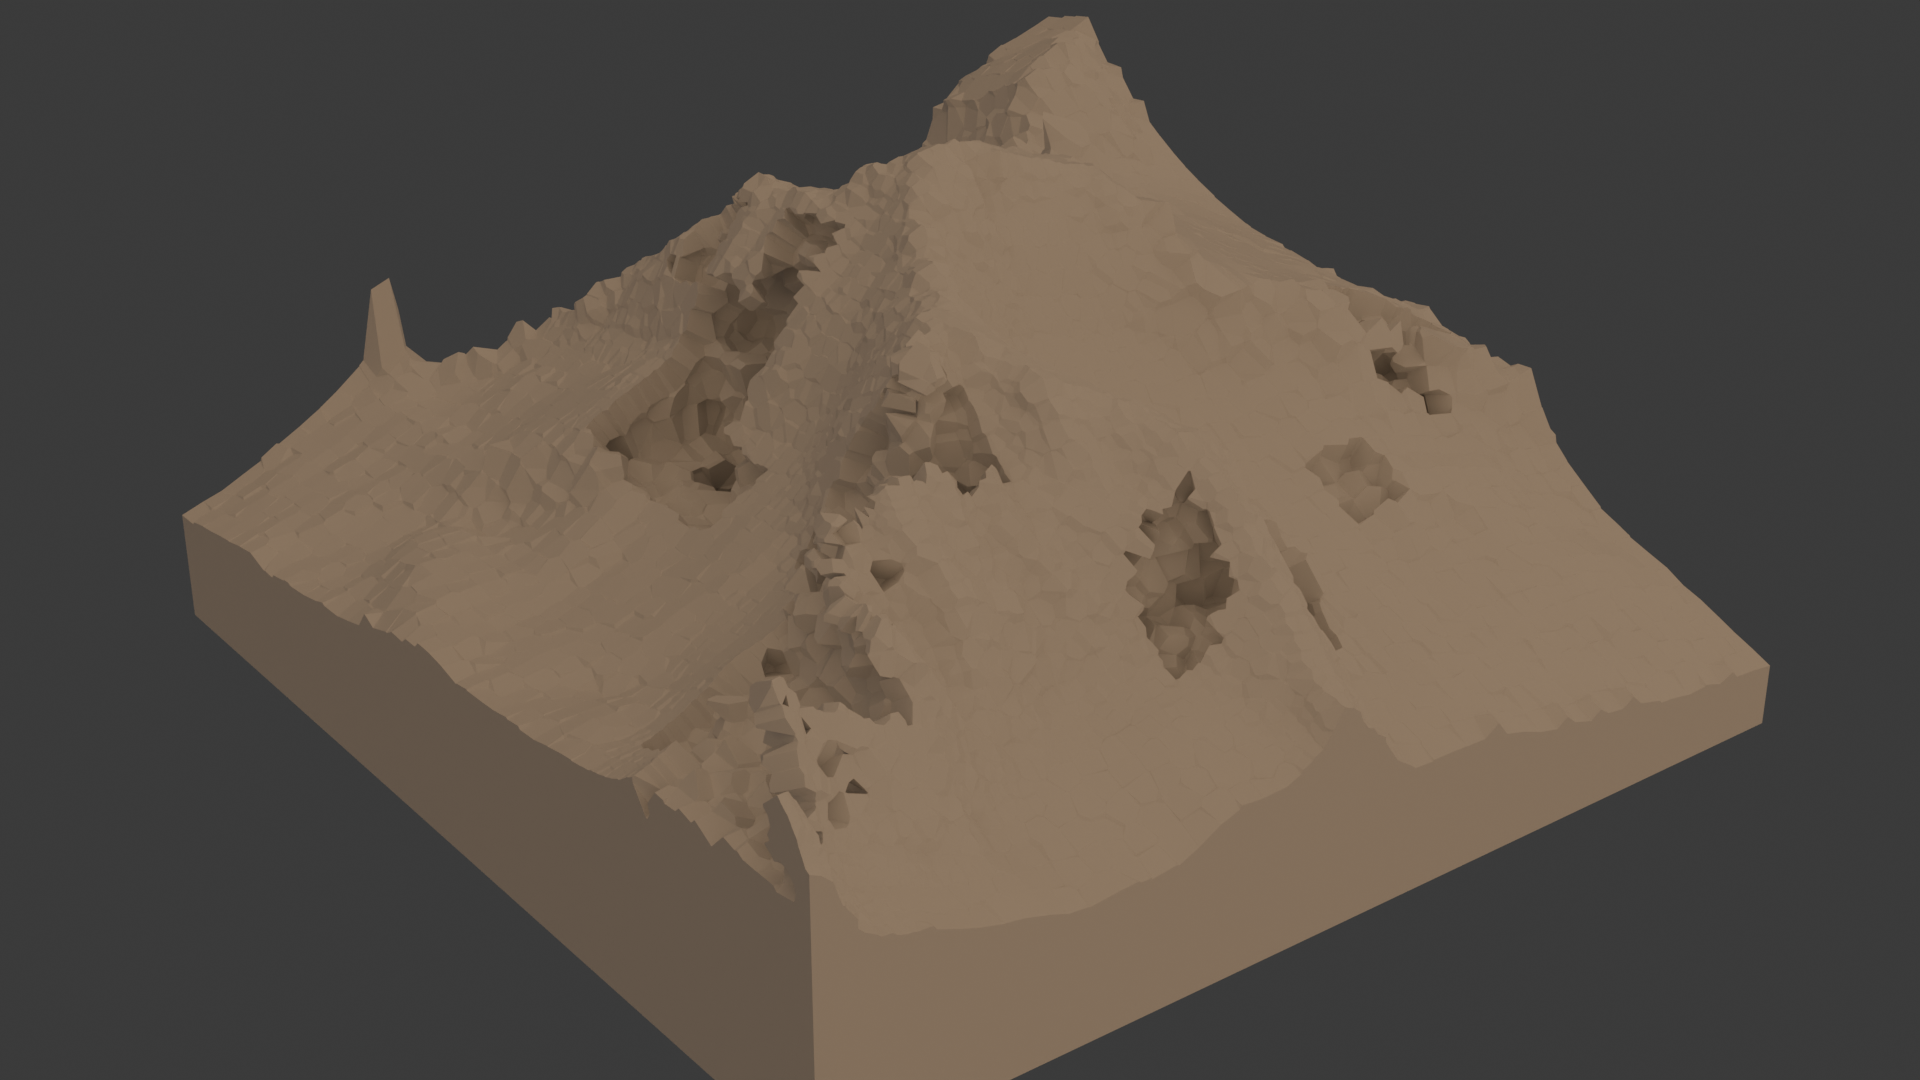
\includegraphics[width=0.48\linewidth]{Results/Renders/gramnite400Overview.png}
    }
    \hspace{5pt}
    \subfigure[Eroion simulation after 400 paths on reinforced granite. Zoomed]{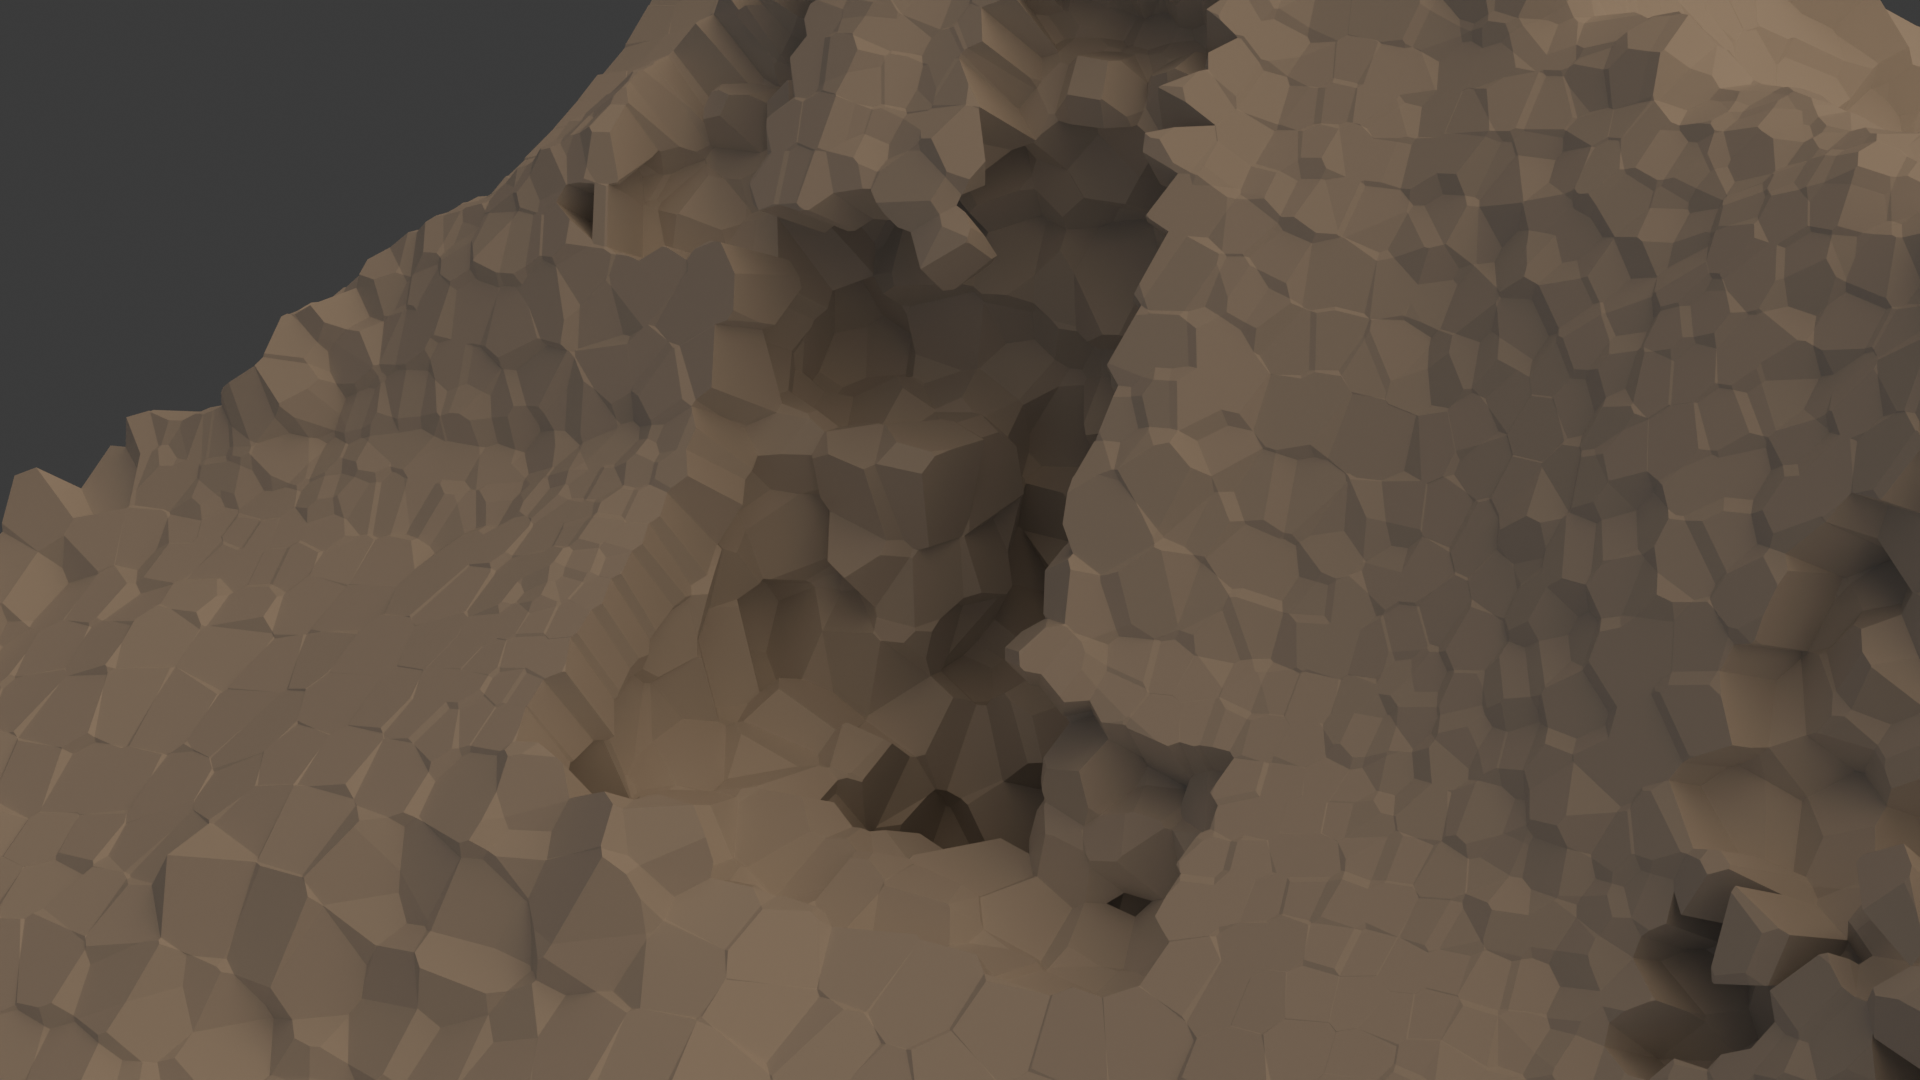
\includegraphics[width=0.48\linewidth]{Results/Renders/graniteDetail.png}}
    \hfill
    \subfigure[Eroion simulation after 400 paths on reinforced marble. Overview]{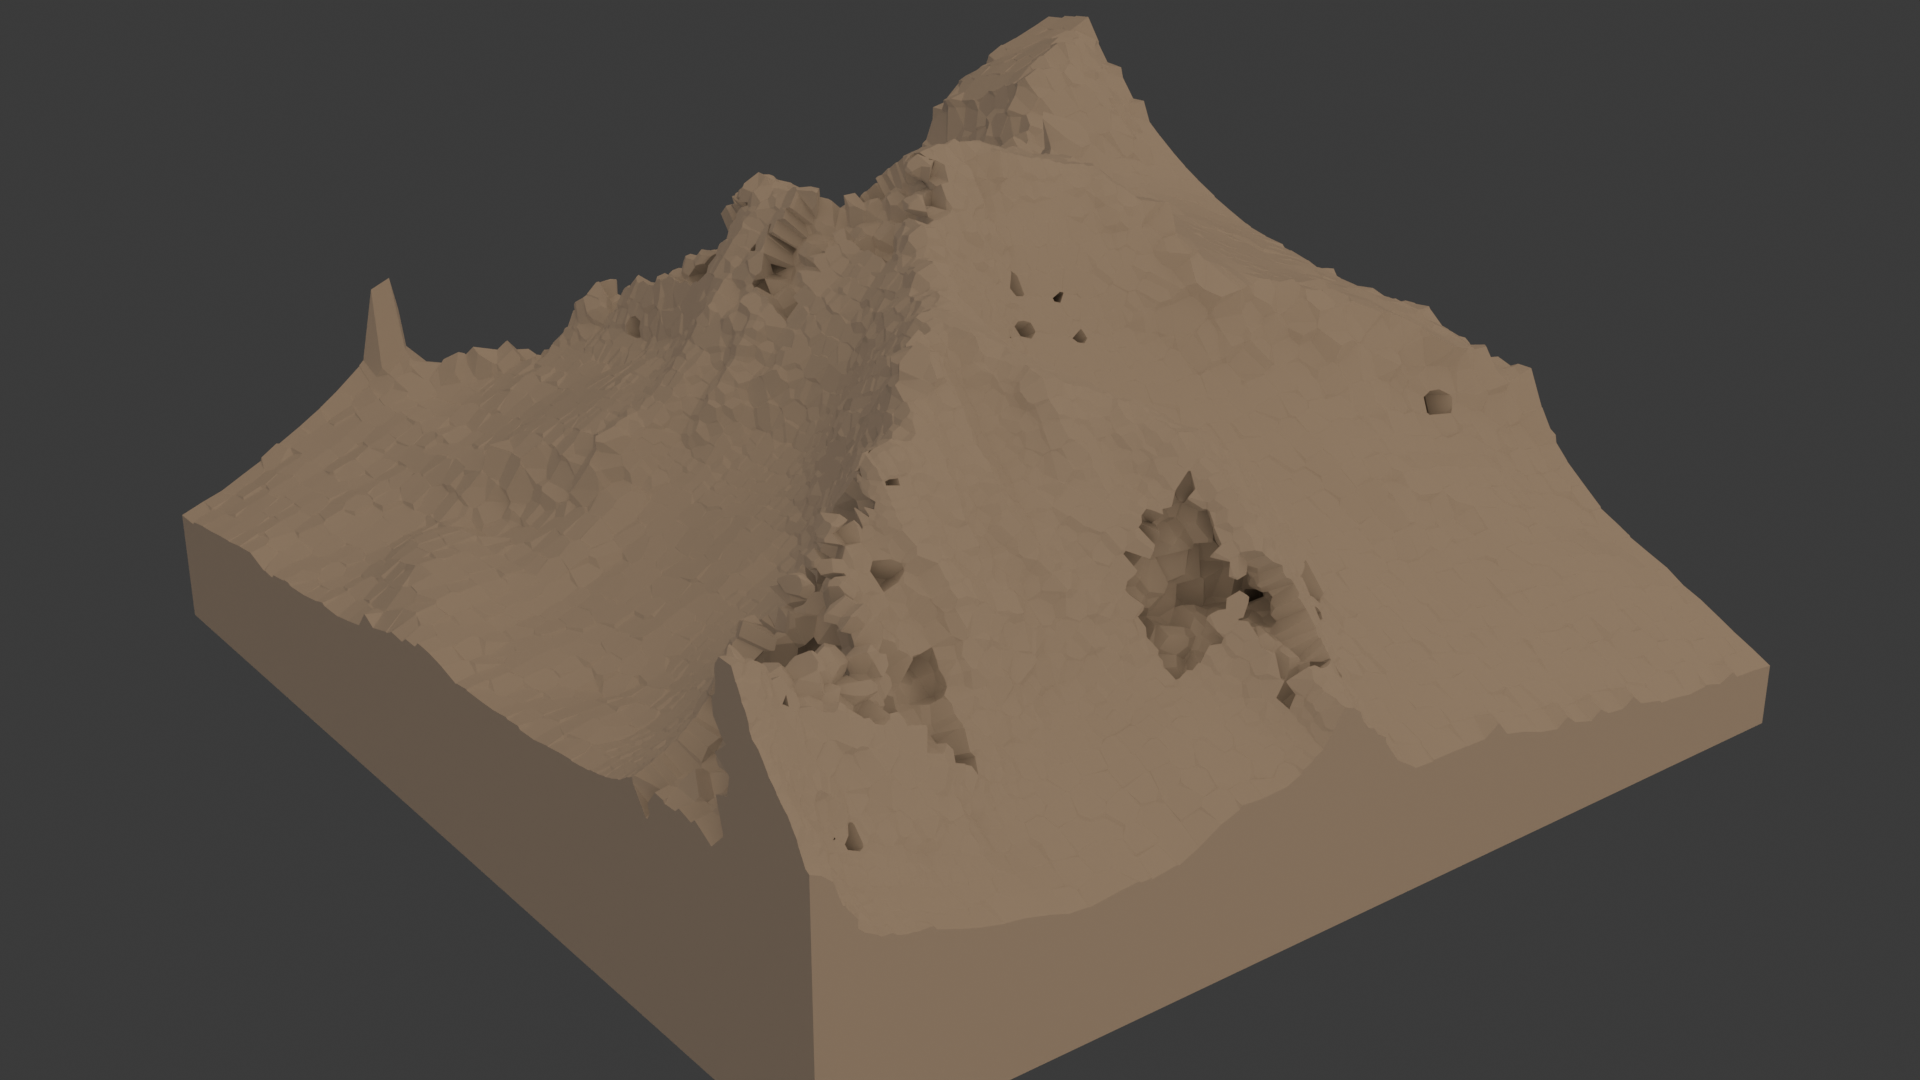
\includegraphics[width=0.48\linewidth]{Results/Renders/marble400Overview.png}}
    \hspace{5pt}
    \subfigure[Eroion simulation after 400 paths on reinforced marble. Zoomed]{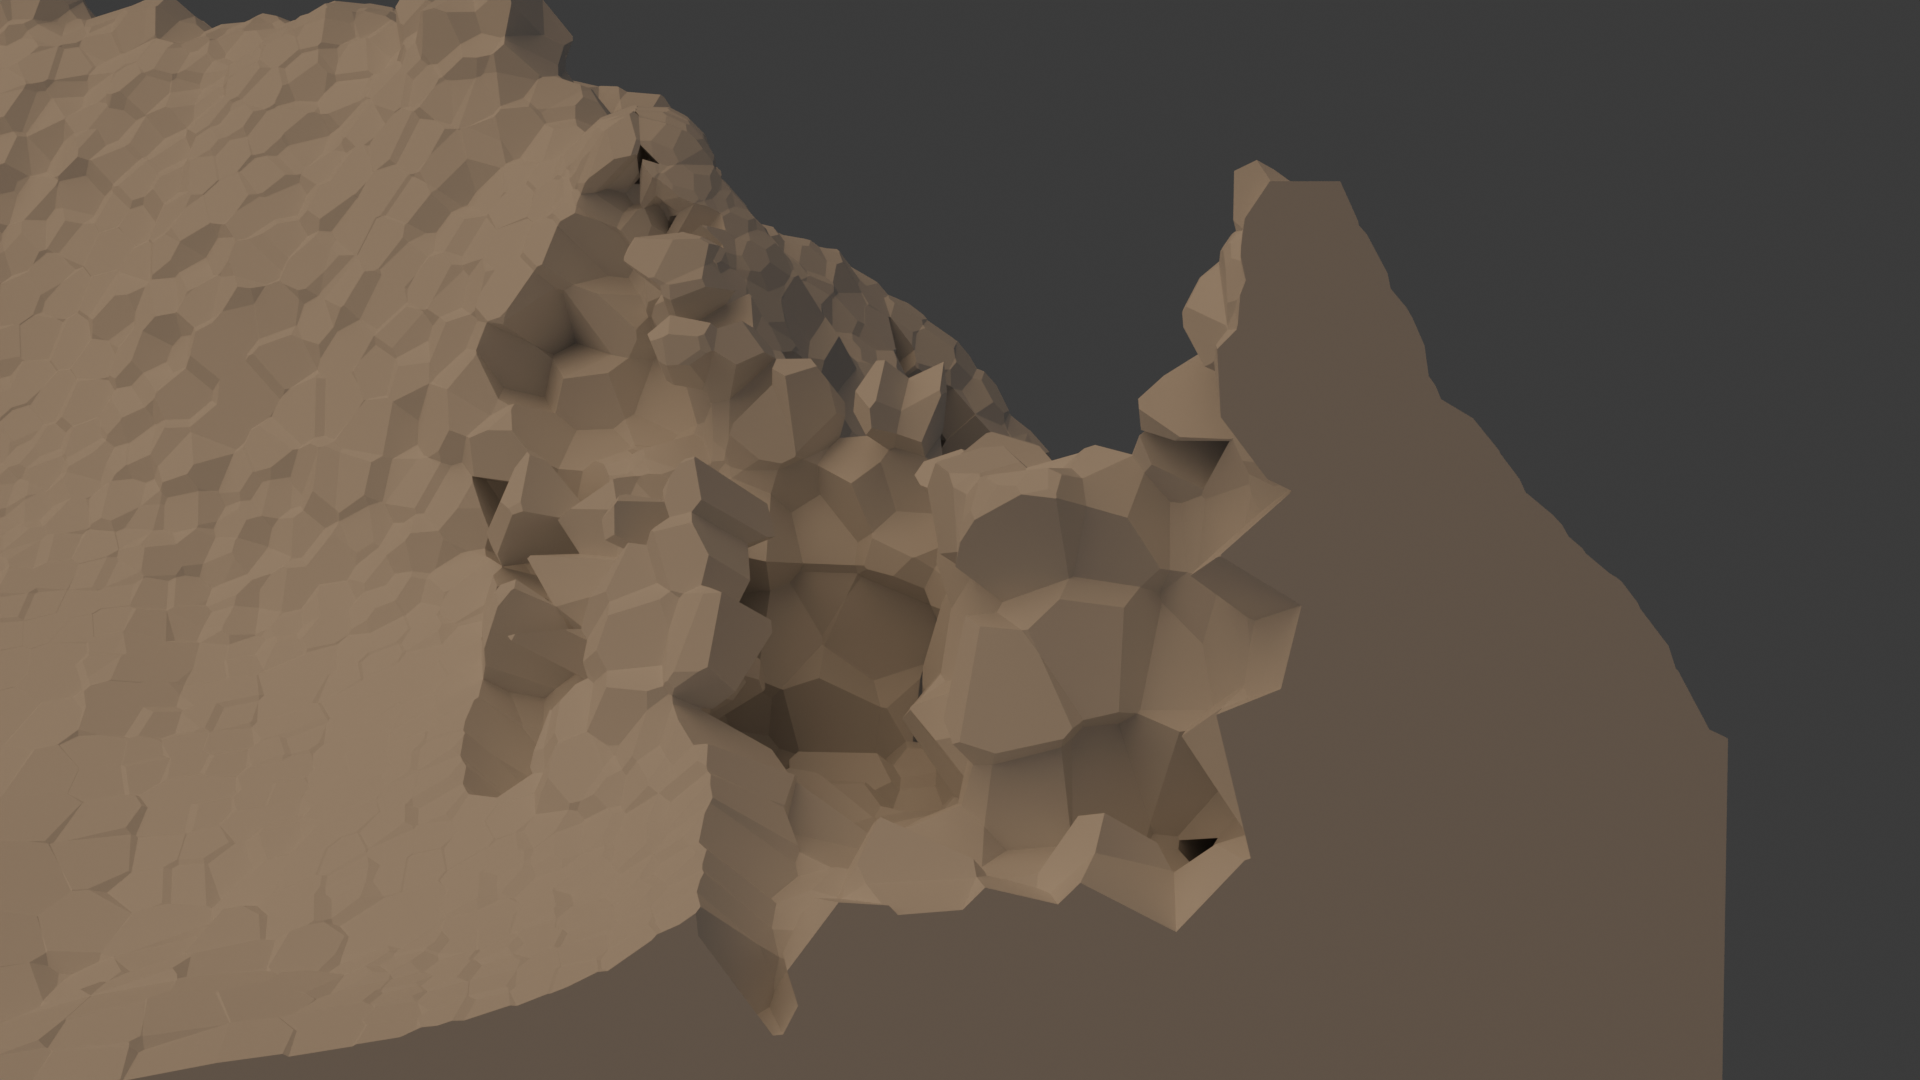
\includegraphics[width=0.48\linewidth]{Results/Renders/marbleDetail.png}}
    \hfill
    \subfigure[Eroion simulation after 400 paths on reinforced sandstone. Overview]{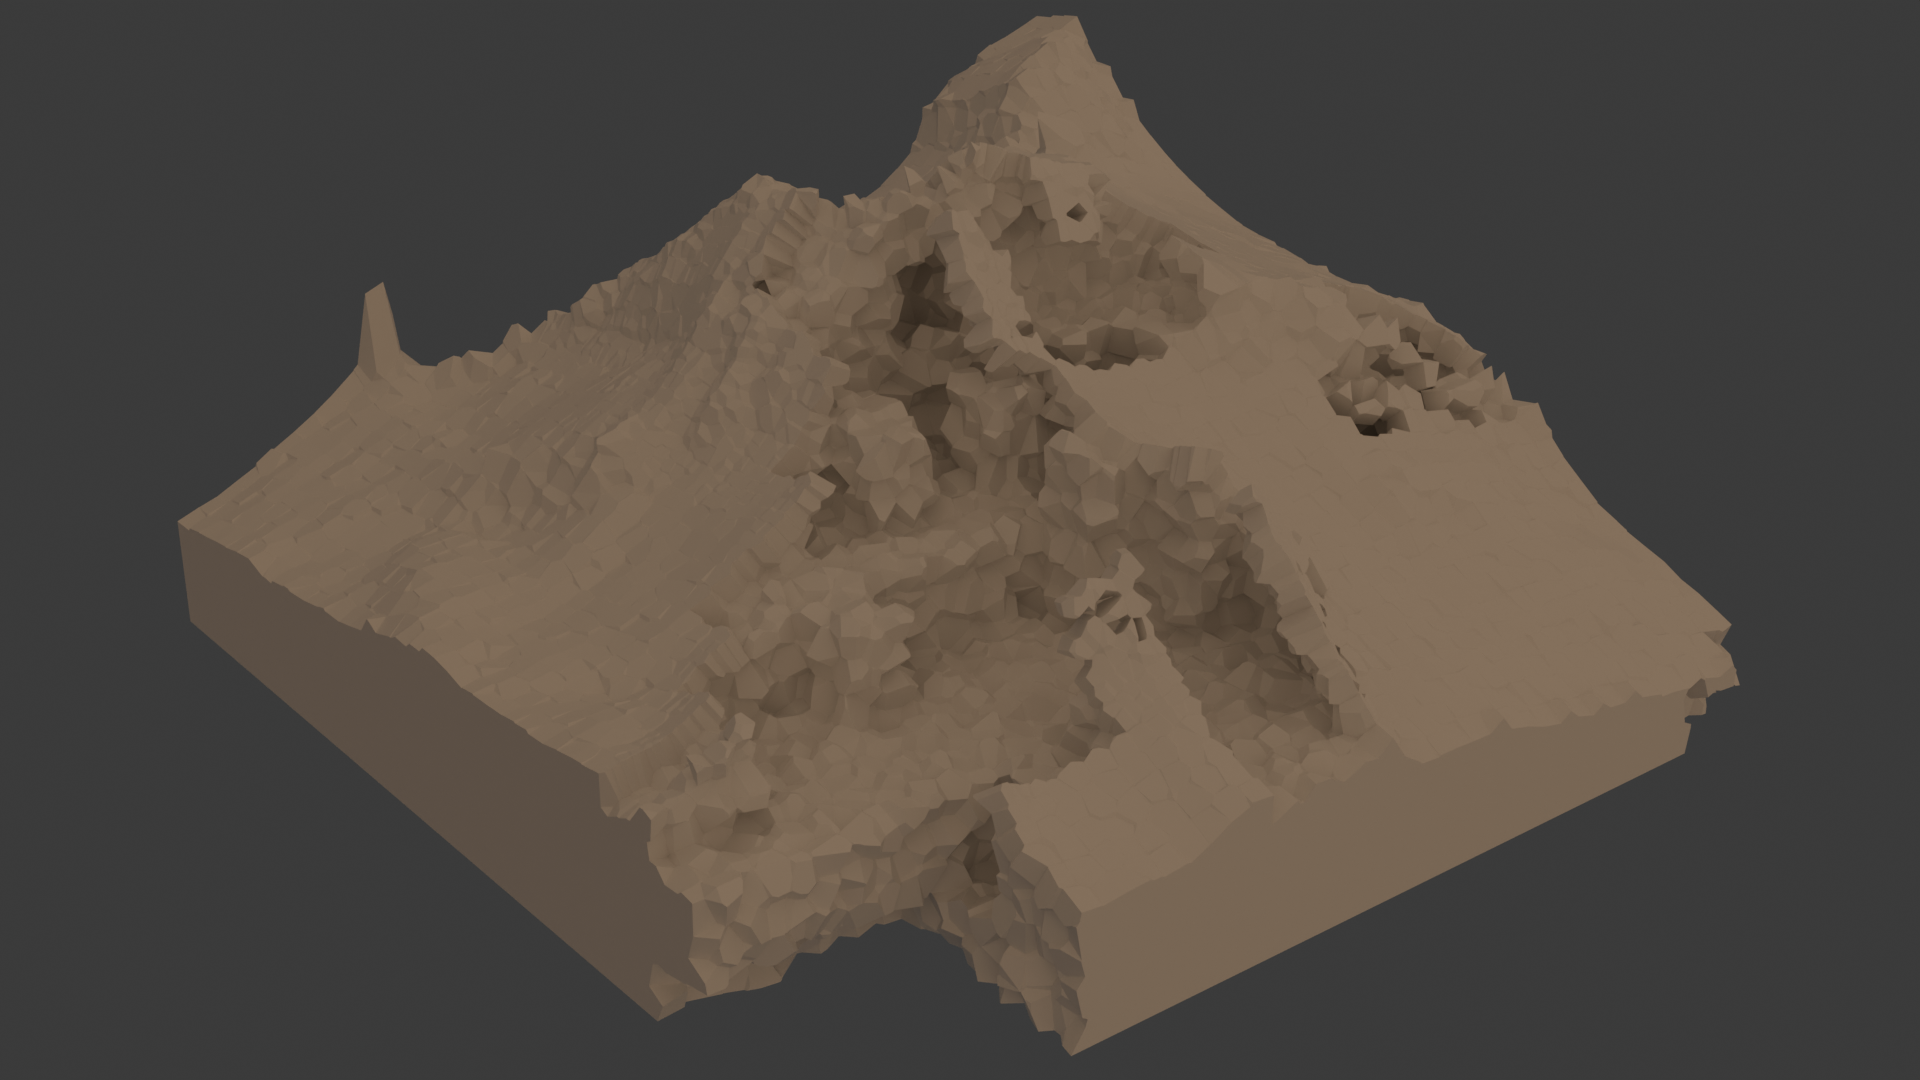
\includegraphics[width=0.48\linewidth]{Results/Renders/sandstone400Overview_4.png}}
    \hspace{5pt}
    \subfigure[Eroion simulation after 400 paths on reinforced sandstone. Zoomed]{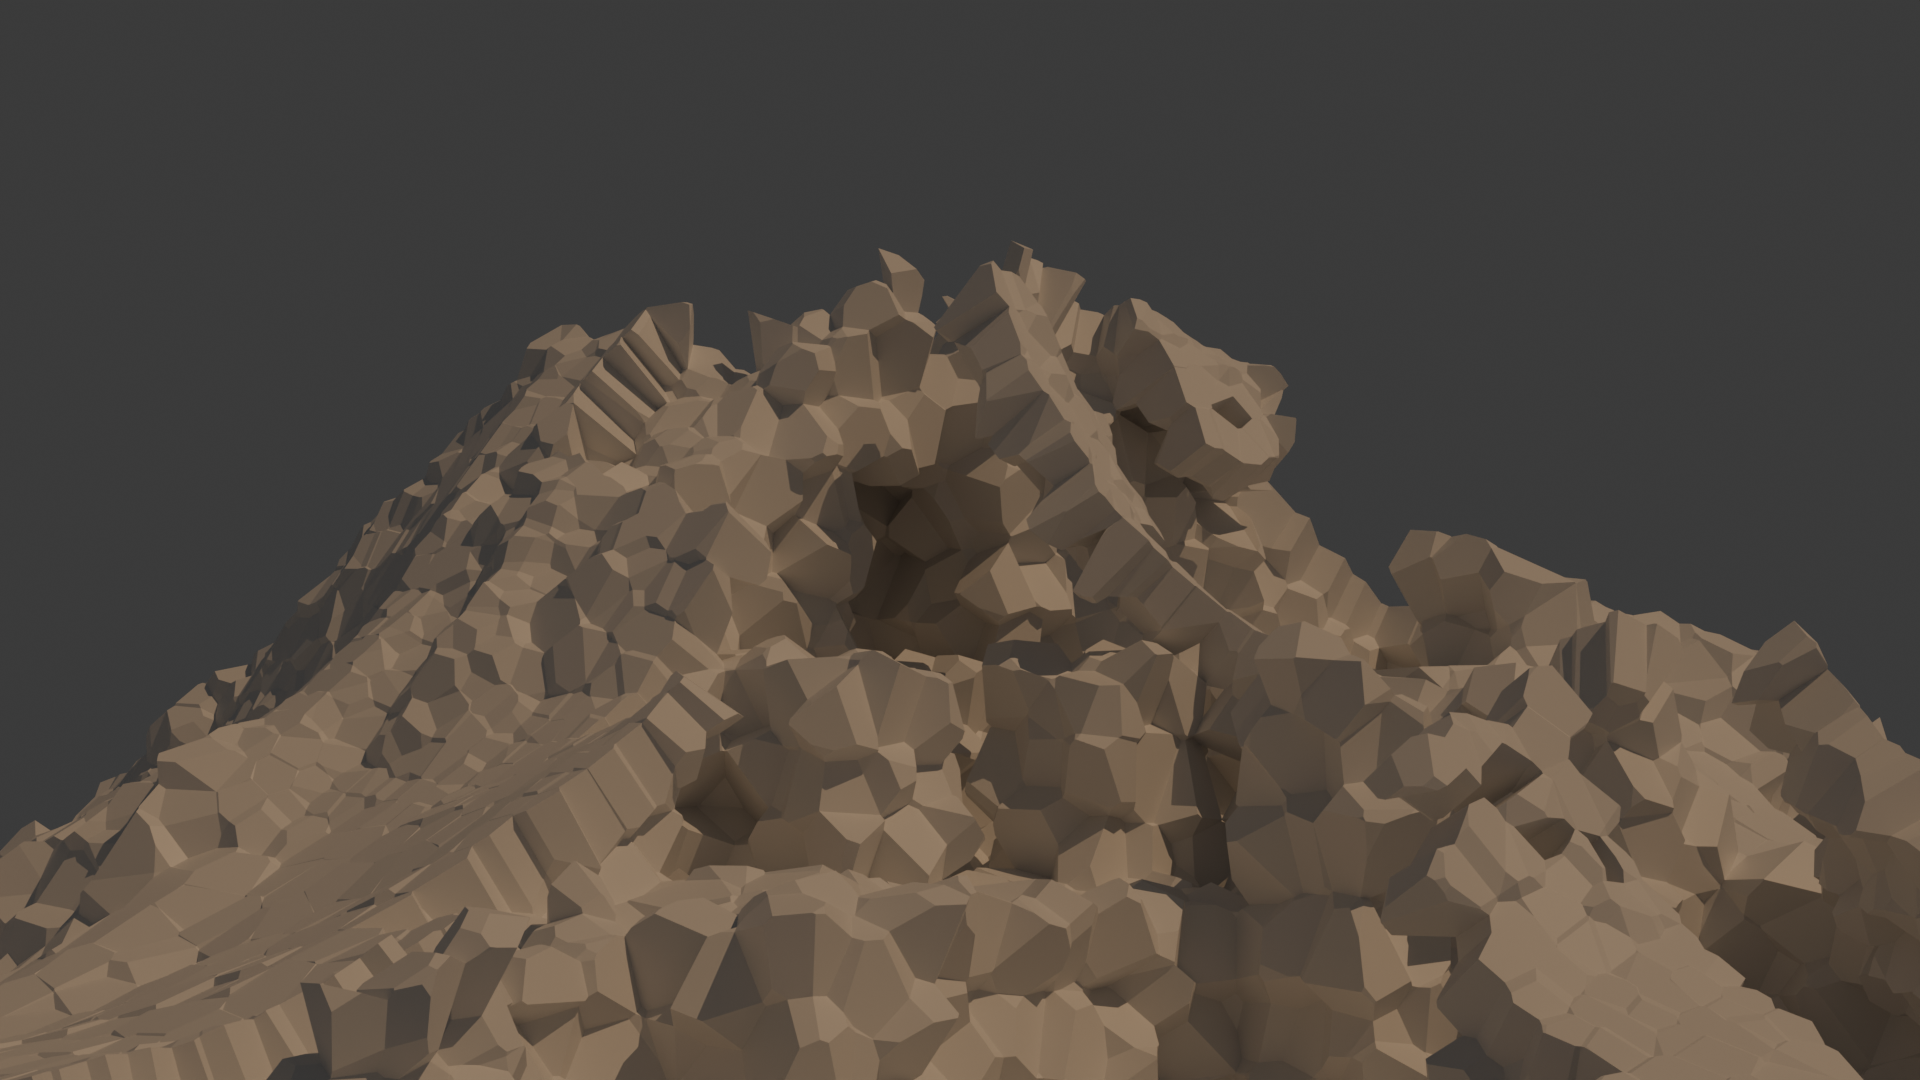
\includegraphics[width=0.48\linewidth]{Results/Renders/sandstoneDetail.png}}


    \caption{Erosion simulation after 400 paths on different reinforced materials.
    All images have been rendered on Blender using the exported eroded terrain 
    from our application} 
    \label{fig:meterialComparison}
\end{figure}


%\subsubsection{Failure Parameter Tunning}
\subsubsection{Computational Time Results}

During all of our experiments, we also collected data on their time 
to compute. Unlike the base algorithm, separating parts is not the 
most expensive task of this method, as the most expensive one is 
recomputing the system, which happens every time a link is broken. Link 
removal is much whole more common than cell removals, so they are expected to 
appear through each state of the erosion simulation process. Technically, 
the probability of a link breaking depends on the stress of the system, 
but the relationship between the number of paths executed and the 
probability of a link breaking is not that simple to compute. The only clear 
relationship between the amount of paths already computed and the 
cost of the next path is the number of remaining cells; the fewer 
cells there are, the cheaper it is to compute the state of the system.

\vspace{10pt}

Regarding the computational cost, we performed an experiment 
using reinforced sandstone that provided really useful information. 
We tried 15 consecutive rounds of 25 paths each (for a total of 375 paths) 
measuring the time they took to compute and the remaining cells after 
the computation. In figure \ref{fig:computationTimePerPath} we can see 
that the average time to compute a water path varies a lot for each 
consecutive round but with a downward trend in the last four 
paths. We can relate this downward trend to the number of cells 
seen in figure \ref{fig:cellNum}: the last four rounds have a marked 
decrease in the number of cells, so cheaper computations are expected.

\begin{figure}
    \centering 
    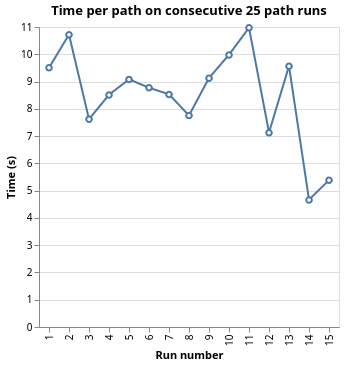
\includegraphics[scale = 0.35]{Results/timePerPathSandstone.png}
    \caption{Time per path on different consecutive 25 path runs using 
    the reinforced sandstone material}
    \label{fig:computationTimePerPath}
\end{figure}
\begin{figure}
    \centering 
    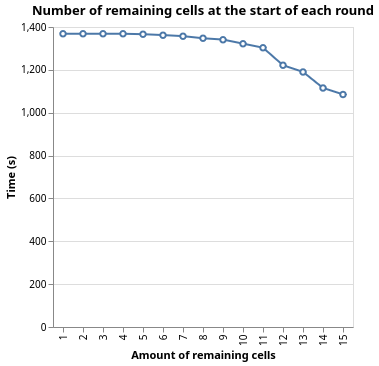
\includegraphics[scale = 0.35]{Results/cellsPerRound.png}
    \caption{Remaining cells at the begining of each consecutive round 
    of 25 paths}
    \label{fig:cellNum}
\end{figure}
\subsection{Method Comparison}

Finally, after conducting all experiments, we are ready to compare 
the results of the erosion process using the base method and the 
method including the mechanical model. In order to do a fair comparison, 
we compared the results on the \textit{Aneto} terrain using a 50x50 grid 
for the heightfield and a 3x3x3 block grid to perform subsampling.

\vspace{10pt}

The first important difference is the computational cost. Different 
experiments on different materials using the mechanical model required 
multiple seconds per path, while our test on the same 
model using the base method took only tens of microseconds. Fortunately, 
our improved method required fewer paths to erode the model: we could 
appreciate the results with just a hundred paths, while the base method 
required at least a few thousand. This difference in the number of paths 
required to erode helps reduce the computational cost of the 
improved method (as we do not need to perform that many paths).

\vspace{10pt}

After going over the cost comparison, we have to mention the most important
part: the results of the erosion simulation. The main problem with 
the base algorithm is that it generates multiple structures that are 
almost floating, only connected to the terrain through a thin chain 
of rocks. On the other hand, our improved method does not produce these 
almost floating chunks, and the resulting terrain appears to be much 
more physically stable. 

\begin{figure}
    \centering

    \subfigure[Aneto terrain after applying the base algorithm (without mechanical model).
    A big portion of the bottom of the terrain is removed but parts of the surface 
    still survive almost floating]{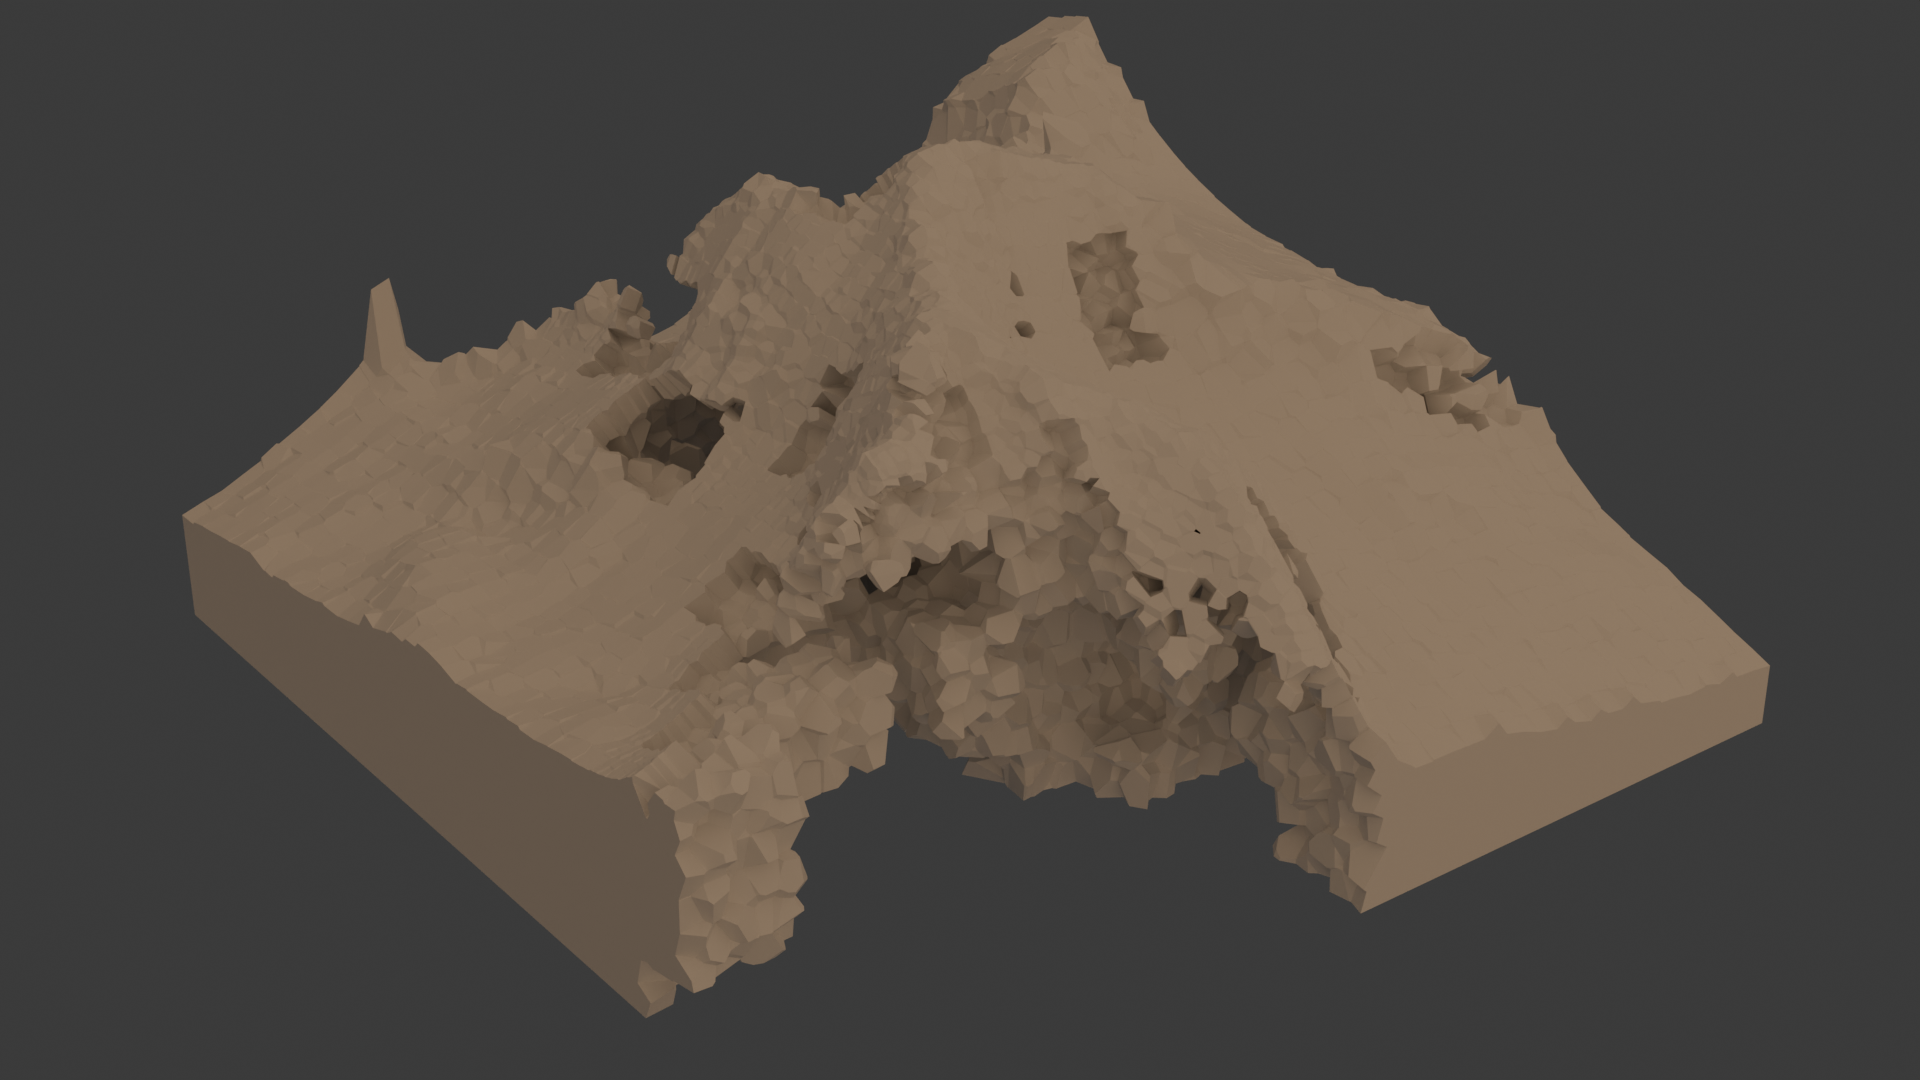
\includegraphics[width=0.45\linewidth]{Results/Renders/baseErosionOverview1.png}
    }
    \hspace{20pt}    
    \subfigure[Aneto mountain after applying the mechanical model using our reinforced sandstone.
    In this case the surface of the mountain has mostly fallen along the bottom section of the terrain]{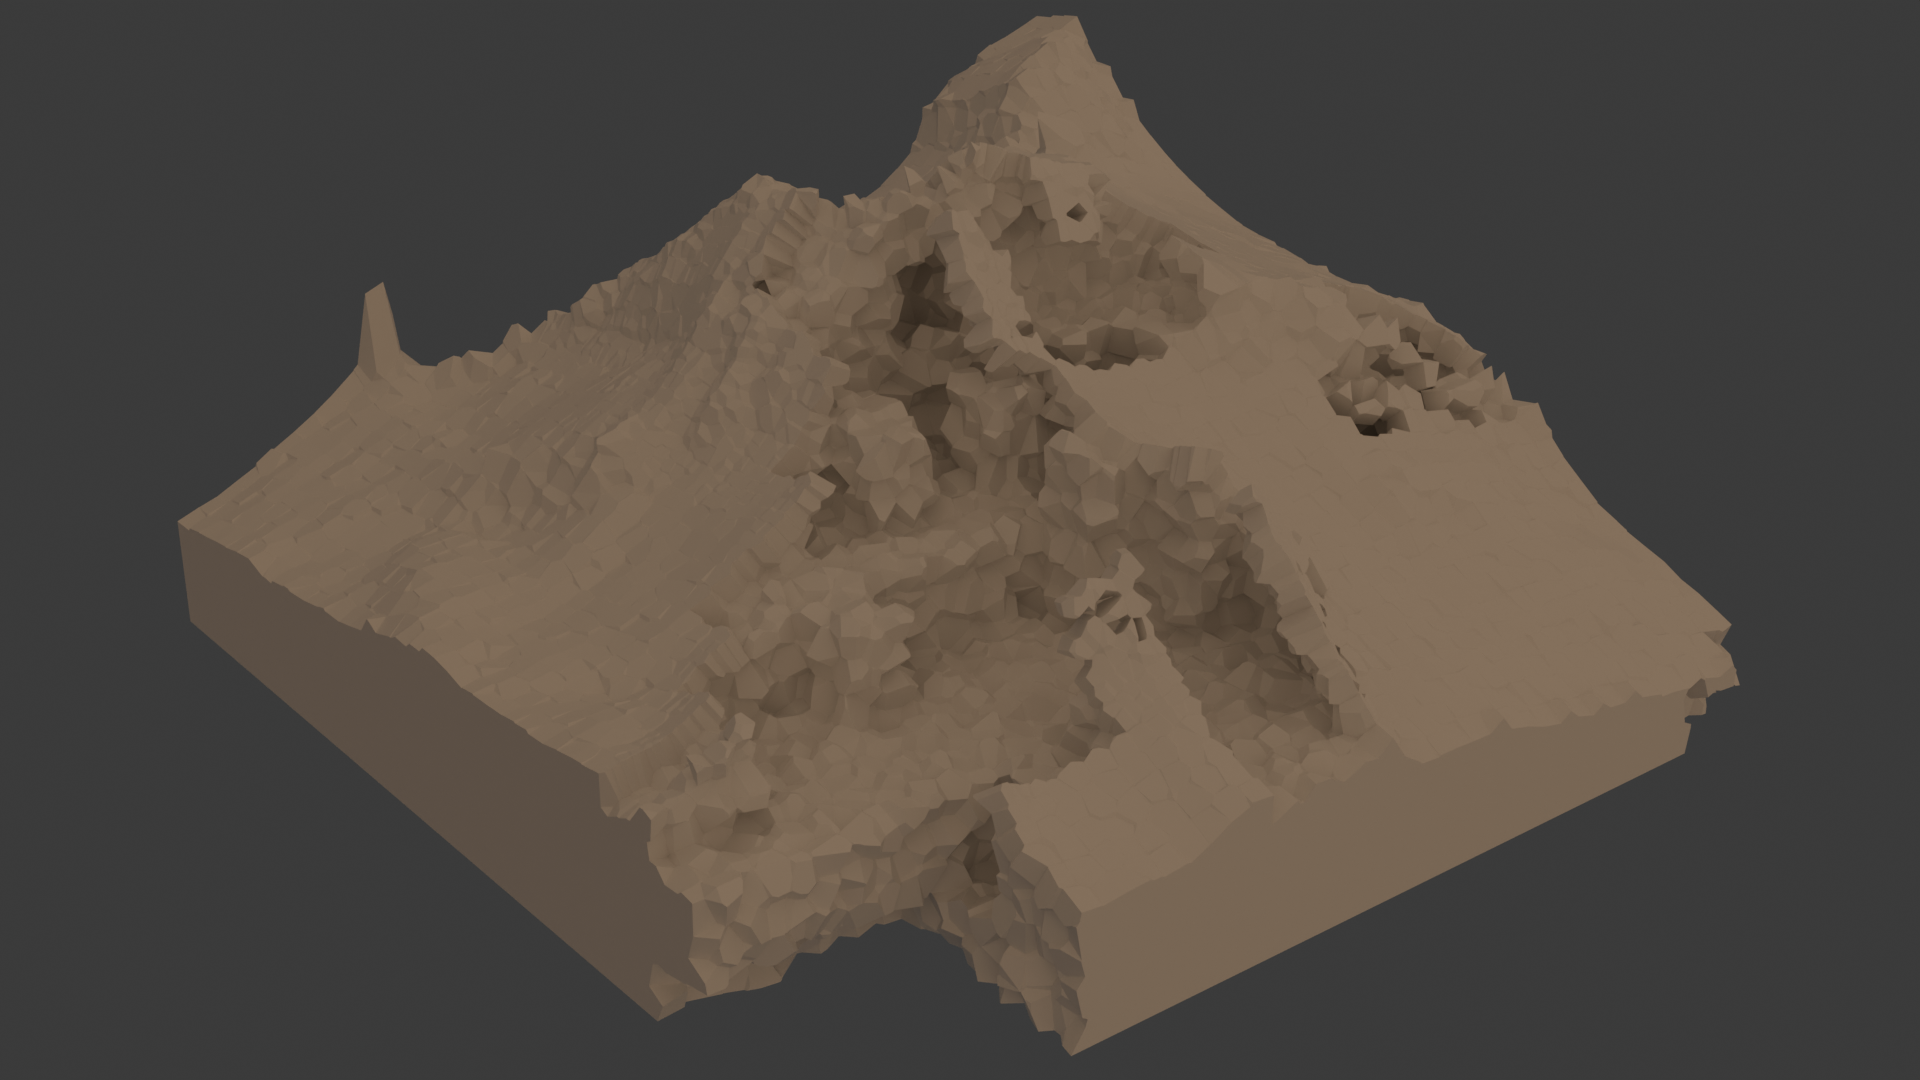
\includegraphics[width=0.45\linewidth]{Results/Renders/sandstone400Overview_4.png}}

    \caption{Figure comparing the base algorithm with our improved algorithm using 
    reinforced sandstone as a material. All images have been rendered using 
    Blender after exporting the eroded terrain} 
    \label{fig:baseVsMech}
\end{figure}


\newpage


\chapter{Conclusions}

In this project, we successfully improved the previous work of 
\cite{10.2312:ceig.20241139}, adding a mechanical model to simulate 
the physical properties of terrains and better reproduce erosion 
processes. Moreover, we also made improvements in the voronoi tessellation and 
added a low-resolution layer to speed up the erosion simulation. 
All added improvements with respect to the previous project contributed 
to the quality and realism of the final eroded terrain, which 
has the potential to be used to produce realistic landscapes in virtual 
scenes. 

\vspace{10pt}

Despite all of this, there is some work that can still be done to improve 
this project. First, the goal of this thesis was just to improve 
the previous method and add the physical considerations. In this 
project, we did not have the intention to provide tools for authoring 
terrains using our technique, and we just provided some tools for 
experimentation and debugging. If we want this method to be available for 
digital artists, we would need to port our algorithm to another application 
better suited for these tasks. Furthermore, the current lighting 
method of our application is not suited to produce high-quality 
visuals, so a port to another application that does implement 
better lighting will also improve this aspect.

\vspace{10pt}

Second, we have researched a little about improvements on the solver 
for systems of equations. There are some steps that can be done to improve 
that part, like using a GPU solver or recomputing just the relevant 
parts of the system when a portion of the terrain changes, avoiding a 
full computation each time. We did not have the time to test these improvements, 
so we leave them for future work. Additionally, even if the system of 
equations is the heaviest part of the project, it is not the only one 
that can be optimized; multiple parts of the code can be improved and, 
especially, parallelized in order to increase the algorithm efficiency.

\vspace{10pt}

The last potential improvement of this project has to do with parameter tuning. 
This thesis proposed multiple improvements, so we had to test a wide 
variety of parameters and methods to have a good understanding of how 
our techniques work and how they are compared against other methods. A 
possible extension of our work could consist in testing and comparing 
more materials and better tuning the parameters that control the link 
damage.  

\vspace{10pt}

Finally, and to end this project, we would like to thank both 
Oscar Argudo for tutoring this thesis and Diego Mateos for 
providing the base method this project is based on. Without their 
contributions this project would have not been possible.
\newpage
\nocite{*}
\printbibliography


\end{document}